%----------------------------------------------------------------------------------------
%   Доорх хэсгийг өөрчлөх шаардлагагүй
%----------------------------------------------------------------------------------------
%!TEX TS-program = xelatex
%!TEX encoding = UTF-8 Unicode
%----------------------------------------------------------------------------------------
%   Доорх хэсгийг өөрчлөх шаардлагагүй
%----------------------------------------------------------------------------------------
%!TEX TS-program = xelatex
%!TEX encoding = UTF-8 Unicode
\documentclass[12pt,a4paper]{report}

\usepackage{fontspec,xltxtra,xunicode}
\setmainfont[Ligatures=TeX]{Times New Roman}
\setsansfont{Arial}
\setmonofont{Consolas}

% \usepackage[utf8x]{inputenc}
% \usepackage[mongolian]{babel}
%\usepackage{natbib}
\usepackage[a4paper,margin=2.5cm]{geometry}
%\usepackage{fancyheadings} fancyheadings is obsolete: replaced by fancyhdr. JL
\usepackage{fancyhdr}
\usepackage{float}
\usepackage[section]{placeins}
\usepackage{afterpage}
\usepackage{xcolor}

\setlength{\headheight}{15pt}

\usepackage{graphicx}
\usepackage{amsmath,amssymb,amsbsy}
\usepackage{dcolumn,array}
\usepackage{tocloft}
\usepackage{dics}
\usepackage{nomencl}
\usepackage{upgreek}
\newcommand{\argmin}{\arg\!\min}
\usepackage{mathtools}
\usepackage[hidelinks]{hyperref}
\usepackage{longtable}
\usepackage{booktabs}
\usepackage{array}
\usepackage{ragged2e}
\newcolumntype{L}[1]{>{\RaggedRight\arraybackslash}p{#1}}
\setlength{\LTleft}{0pt}
\setlength{\LTright}{0pt}
\AtBeginDocument{%
  \justifying
  \tolerance=3000
  \emergencystretch=3em
  \hyphenpenalty=200
  \exhyphenpenalty=200
}
\newcommand{\placeholderfigure}[2]{%
  \begin{figure}[H]
    \centering
    \fbox{\parbox{0.8\textwidth}{\centering #2}}
    \caption{#1}
  \end{figure}
}


\usepackage{algorithm}
\usepackage{algpseudocode}

\usepackage{listings}
\DeclarePairedDelimiter\abs{\lvert}{\rvert}%
\makeatletter
\usepackage{caption}
\captionsetup[table]{belowskip=0.5pt}
\usepackage{subfiles}
\renewcommand{\arraystretch}{1.25}
\renewcommand{\lstlistingname}{Код}
\renewcommand{\lstlistlistingname}{\lstlistingname ын жагсаалт}

\lstdefinelanguage{JavaScript}{
  keywords={await, async, break, case, catch, class, const, continue, debugger, default, delete, do, else, export, extends, finally, for, function, if, import, in, instanceof, let, new, return, super, switch, this, throw, try, typeof, var, void, while, with, yield},
  keywordstyle=\color{blue}\bfseries,
  ndkeywords={boolean, throw, import, export, true, false, null, undefined},
  ndkeywordstyle=\color{orange}\bfseries,
  identifierstyle=\color{black},
  sensitive=false,
  comment=[l]{//},
  morecomment=[s]{/*}{*/},
  commentstyle=\color{gray}\ttfamily,
  stringstyle=\color{red}\ttfamily,
  morestring=[b]',
  morestring=[b]"
}
\usepackage{color}
\definecolor{codegreen}{rgb}{0,0.6,0}
\definecolor{codegray}{rgb}{0.5,0.5,0.5}
\definecolor{codepurple}{rgb}{0.58,0,0.82}
\definecolor{backcolour}{rgb}{0.99,0.99,0.99}
 
\lstdefinestyle{mystyle}{
    basicstyle=\ttfamily\small,
    backgroundcolor=\color{backcolour},   
    commentstyle=\color{codegreen},
    keywordstyle=\color{magenta},
    numberstyle=\tiny\color{codegray},
    stringstyle=\color{codepurple},
    %basicstyle=\footnotesize,
    breakatwhitespace=false,         
    breaklines=true,                 
    captionpos=b,                    
    keepspaces=false,                 
    numbers=left,                    
    numbersep=10pt,                  
    showspaces=false,                
    showstringspaces=true,
    showtabs=false,                  
    tabsize=2
}
 
\lstset{style=mystyle} 

\let\oldabs\abs
\def\abs{\@ifstar{\oldabs}{\oldabs*}}
\makenomenclature

%----------------------------------------------------------------------------------------
%   Өөрийн мэдээллээ оруулах хэсэг
%----------------------------------------------------------------------------------------

% Дипломийн ажлын сэдэв
\title{Зан үйлд суурилсан дадал хэвшүүлэх систем}
% Дипломын ажлын англи нэр
\titleEng{Behavior Based Habit Formation System}
% Өөрийн овог нэрийг бүтнээр нь бичнэ
\author{Галбаярын Дэлгэрмаа}
% Өөрийн овгийн эхний үсэг нэрээ бичнэ
\authorShort{Г.Дэлгэрмаа}
% Хамтарсан удирдагчийн зэрэг цол овгийн эхний үсэг нэр
\supervisor{Ж.Үйтүмэн}

% СиСи дугаар 
\sisiId{22B1NUM5541}
% Их сургуулийн нэр
\university{МОНГОЛ УЛСЫН ИХ СУРГУУЛЬ}
% Бүрэлдэхүүн сургуулийн нэр
\faculty{МЭДЭЭЛЛИЙН ТЕХНОЛОГИ, ЭЛЕКТРОНИКИЙН СУРГУУЛЬ}
% Тэнхимийн нэр
\department{МЭДЭЭЛЭЛ, КОМПЬЮТЕРЫН УХААНЫ ТЭНХИМ}
% Зэргийн нэр
\degreeName{Бакалаврын судалгааны ажил}
% Суралцаж буй хөтөлбөрийн нэр
\programeName{Программ хангамж (D061302)}
% Хэвлэгдсэн газар
\cityName{Улаанбаатар}
% Хэвлэгдсэн огноо
\gradyear{2026 оны 3 сар}

% \makefrontpage
% \maketitle


\begin{document}

\include{main-pre}

%----------------------------------------------------------------------------------------
%   Дипломын үндсэн хэсэг эндээс эхэлнэ
%----------------------------------------------------------------------------------------
\chapter{УДИРТГАЛ}

Сүүлийн жилүүдэд хүний зан үйл, дадал хэвшлийг өөрчлөхөд дижитал технологийг ашиглах асуудал нь зан үйлийн шинжлэх ухаан болон програм хангамжийн инженерийн огтлолцолд байрлах чухал судалгааны чиглэл болж байна. Эрүүл мэнд, боловсрол, бүтээмж, хувийн зохион байгуулалт зэрэг олон талбар нь давтагдах зан үйлд тулгуурладаг бөгөөд ийм тогтворжсон давталтыг дадал гэж үздэг \cite{ref1}. Дадал нь тодорхой нөхцөл, өдөөгч дохио, давталтын нөлөөгөөр аажмаар автоматжиж, хүний өдөр тутмын шийдвэр гаргалт, үйл ажиллагаанд тогтвортой нөлөө үзүүлдэг. Иймээс зан үйлийг тогтвортой өөрчлөхөд зөвхөн богино хугацааны сэдэл, сануулга хангалтгүй бөгөөд дадал үүсэх суурь механизмыг ойлгосон системийн шийдэл шаардлагатай.

Дадал үүсэх үйл явцыг тайлбарлахад Duhigg-ийн өдөөгч дохио--үйлдлийн хэвшил--урамшууллын загвар, Clear-ийн өдөөгч дохио--хүсэл тэмүүлэл--хариу үйлдэл--урамшууллын загвар, мөн Fogg-ийн зан үйлийн загвар өргөн хэрэглэгддэг \cite{ref2,ref3,ref4}. Эдгээр онол нь зан үйлийг ямар нөхцөлд эхлүүлэх, тогтвортой давтуулах, улмаар автоматжуулахыг тайлбарладаг тул дадал төлөвшүүлэх дижитал системийн логикийг тодорхойлоход онолын суурь болдог.

Өнөөгийн дадал хянах олон систем сануулга өгөх, гүйцэтгэл бүртгэх, цуваа болон статистик мэдээлэл харуулах зэрэг нийтлэг функцтэй боловч дадал үүсэх зан үйлийн механизмыг цогц байдлаар тусгаж чаддаггүй. Судалгаагаар ийм төрлийн шийдлүүд нь хэрэглэгчийг давталтад дэмжих боловч зарим тохиолдолд системийн сануулга, интерфэйсээс хэт хамааралтай болгох эрсдэлтэйг тэмдэглэсэн байдаг \cite{ref5}. Үүнээс гадна зан үйлийн онолыг системийн архитектур, өгөгдлийн загвар, функциональ логик, алгоритмын түвшинд хөрвүүлэн хэрэгжүүлэх инженерчлэлийн судалгаа харьцангуй хязгаарлагдмал байна.

Иймд энэхүү судалгаагаар дадал төлөвшлийн мөчлөгт тулгуурлан хэрэглэгчийн дадал үүсэх, бэхжих үйл явцыг дэмжих зан үйлд суурилсан програм хангамжийн системийн загвар боловсруулна. Уг системд өдөөгч дохио, хүсэл тэмүүлэл, хариу үйлдэл, урамшуулал гэсэн бүрэлдэхүүнүүдийг системийн функц, өгөгдлийн загвар, алгоритмын логиктой уялдуулан авч үзнэ. Өөрөөр хэлбэл, энэ ажил нь зөвхөн дадал бүртгэх энгийн систем бус, харин хэрэглэгчийн зан үйлийг нөхцөл байдалд суурилсан сануулга, сэдлийн дэмжлэг, төвөгшил багатай гүйцэтгэл, оновчтой урамшууллын механизмаар дамжуулан тогтвортой төлөвшүүлэх системийн шийдлийг санал болгож байгаагаараа онцлог юм.

\section{Судалгааны зорилго}

Энэхүү судалгааны ажлын зорилго нь дадал төлөвшлийн мөчлөгт тулгуурлан хэрэглэгчийн дадал хэвшил тогтох үйл явцыг дэмжих зан үйлд суурилсан програм хангамжийн системийн загвар, архитектур, системийн зохиомж, туршилтын загварыг боловсруулахад оршино.

\section{Судалгааны зорилтууд}

Дээрх зорилгыг хэрэгжүүлэхийн тулд дараах зорилтуудыг дэвшүүлэв.

\begin{enumerate}
    \item Дадал үүсэх механизм, дадал төлөвшлийн мөчлөг, Фоггийн зан үйлийн загвар, итгүүлэн нөлөөлөх технологийн онолын үндсийг судлах.
    \item Одоо ашиглагдаж буй дадал хянах системүүдийн онцлог, давуу тал, хязгаарлалтыг харьцуулан шинжлэх.
    \item Зан үйлд суурилсан дадал төлөвшүүлэх системийн үзэл баримтлал, функциональ болон функциональ бус шаардлагыг тодорхойлох.
    \item Өдөөгч дохио, хүсэл тэмүүлэл, хариу үйлдэл, урамшуулал зэрэг бүрэлдэхүүнүүдийг системийн функц, өгөгдлийн загвар, алгоритмын логиктой уялдуулан загварчлах.
    \item Дадлын хүчийг автоматжилтын хэмжүүр болон зан үйлийн үзүүлэлтүүдийг хослуулан үнэлэх модель боловсруулах.
    \item Боловсруулсан шийдэлд тулгуурлан системийн туршилтын загварыг хэрэгжүүлж, үр нөлөөг үнэлэх.
\end{enumerate}

\section{Судалгааны асуулт}

Энэхүү судалгааны ажил нь дараах үндсэн асуултуудад хариулахыг зорьж байна.

\textbf{СА-1.} Дадал төлөвшлийн мөчлөг, Фоггийн зан үйлийн загвар, итгүүлэн нөлөөлөх системийн зохиомжийн зарчмуудыг зан үйлд суурилсан програм хангамжийн системийн архитектур, өгөгдлийн загвар, үндсэн алгоритмын түвшинд хэрхэн хэрэгжүүлж болох вэ?

\textbf{СА-2.} Дадлын хүчийг автоматжилтын хэмжүүр болон зан үйлийн дэмжих үзүүлэлтүүдийг хослуулан хэрхэн үнэлж болох вэ?

\textbf{СА-3.} Нөхцөл байдалд суурилсан сануулга, төвөгшлийг бууруулах дэмжлэг, эргэцүүлсэн урамшууллыг хослуулсан туршилтын загвар нь хэрэглэгчийн дадал төлөвшилд хэрхэн нөлөөлөх вэ?

\section{Судалгааны ач холбогдол}

Энэхүү ажил нь онолын, практик болон инженерчлэлийн ач холбогдолтой.

Онолын ач холбогдлын хувьд, дадал үүсэх зан үйлийн онолыг програм хангамжийн системийн загварчлалтай уялдуулан авч үзэж, дадал төлөвшлийн мөчлөг болон дадлын хүчний ойлголтыг системийн логикт буулгах оролдлого хийснээрээ ач холбогдолтой.

Практик ач холбогдлын хувьд, уг судалгааны үр дүнд боловсруулагдах системийн загвар нь эрүүл хэвшил, суралцах дадал, бүтээмж, хувийн зохион байгуулалт зэрэг зан үйлийг дэмжих дижитал шийдэл боловсруулах суурь болно.

Инженерчлэлийн ач холбогдлын хувьд, зан үйлийн онолыг системийн шаардлага, өгөгдлийн бүтэц, алгоритм, архитектур, системийн зохиомжтой уялдуулан хэрэгжүүлэх жишиг загвар болох боломжтой.

\section{Судалгааны арга зүй}

Судалгаанд дараах үндсэн аргуудыг ашиглана.

Нэгдүгээрт, онолын судалгааны аргаар дадал үүсэх онол, зан үйлийн өөрчлөлтийн загвар, итгүүлэн нөлөөлөх технологи, дадлын хүчийг хэмжих аргуудтай холбоотой бүтээлүүдийг судалж, онолын үндэслэлийг тодорхойлно.

Хоёрдугаарт, харьцуулсан шинжилгээний аргаар одоо ашиглагдаж буй дадал хянах системүүдийн онцлог, давуу тал, хязгаарлалтыг шинжилнэ.

Гуравдугаарт, системийн загварчлалын аргаар онолын хандлагуудыг системийн архитектур, өгөгдлийн бүтэц, функциональ шаардлага, алгоритмын логиктой уялдуулан загварчилна.

Дөрөвдүгээрт, програм хангамжийн хөгжүүлэлтийн аргаар боловсруулсан шаардлага, архитектур, системийн зохиомжийн дагуу туршилтын загварыг хэрэгжүүлнэ.

Тавдугаарт, туршилт ба үнэлгээний аргаар системийн хэрэглээний өгөгдөл, гүйцэтгэлийн бүртгэл, автоматжилтын үнэлгээ, хэрэглэгчийн оролцоонд тулгуурлан системийн үр нөлөөг үнэлнэ.
\chapter{СУДЛАГДСАН БАЙДЛЫН ТОЙМ}

Дадал үүсэх үйл явц болон зан үйлийг дэмжих дижитал системүүдийн талаарх судалгааны анхаарал сүүлийн жилүүдэд нэмэгдэж байна. Ялангуяа гар утсанд суурилсан хэрэглээний програм, мэдэгдлийн систем, ахицыг хянах хэрэгсэл, тоглоомжуулалтын элемент, нөхцөл байдалд суурилсан дэмжлэг зэрэг шийдлүүдийг ашиглан хэрэглэгчийн давтагдах зан үйлийг дэмжих оролдлогууд өргөжсөн байна. Энэ чиглэлийн судалгаанууд нь нэг талаас дадал үүсэх сэтгэлзүйн болон зан үйлийн механизмыг тайлбарлах, нөгөө талаас тэдгээрийг дижитал орчинд хэрхэн хэрэгжүүлж болохыг тодорхойлоход чиглэж байна. Иймээс энэ бүлэгт дадал үүсэх онолын үндэс, зан үйлийг дэмжих дижитал системүүдийн талаарх өмнөх болон сүүлийн үеийн судалгааг авч үзэж, улмаар уг ажлын судалгааны цоорхойг тодорхойлно.

\section{Дадал үүсэх механизмын талаарх судалгаа}

Дадал үүсэх механизмыг тайлбарлах судалгааны суурь нь зан үйлийн сэтгэл судлалын эртний туршилтуудаас эхтэй. Павловын сонгодог нөхцөлдөлтийн туршилтаар анх саармаг байсан дохио давталтын үр дүнд автомат хариу үйлдэл өдөөж болдгийг харуулсан \cite{pavlov1927}. Харин Скиннерийн оперант нөхцөлдөлтийн судалгаагаар эерэг үр дагавартай үйлдэл дахин давтагдах магадлал нэмэгддэг болохыг тогтоосон \cite{skinner1938}. Эдгээр судалгаанууд нь зан үйл нь орчны өдөөгч дохио болон түүний дараах үр дагавартай уялдан тогтворжиж болдгийг харуулсан анхны онолын суурь болсон бөгөөд орчин үеийн дадлын судалгаанд өдөөгч дохио--хариу үйлдлийн холбоо болон зан үйлийг бэхжүүлэх бататгалын механизмын үндсэн ойлголт болж байна.

Дадал нь тодорхой нөхцөлд харьцангуй автоматаар гүйцэтгэгддэг зан үйлийн хэлбэр бөгөөд олон удаагийн давталт, орчны тогтвортой нөхцөл, өдөөгч дохионуудын нөлөөгөөр аажмаар бүрэлддэг \cite{ref1}. Wood ба R\"unger нарын тайлбарласнаар дадал нь орчны дохио болон давтагдах зан үйлийн хооронд үүссэн автомат холбоо бөгөөд хүний зан үйл нь зөвхөн ухамсартай шийдвэр гаргалтаар бус, давтагдсан нөхцөлд автоматаар идэвхждэг хэвшмэл хариу үйлдлээр ч ихээхэн тодорхойлогддог \cite{ref1}.

Lally нар шинэ дадал үүсэх үйл явцыг бодит амьдралын нөхцөлд судлахдаа зан үйл тогтмол давтагдах тусам автоматжилтын түвшин өсдөг боловч энэ өсөлт шугаман бус болохыг тогтоосон \cite{ref6}. Эхний үед автоматжилт харьцангуй хурдан өсөх хандлагатай байдаг бол тодорхой түвшинд хүрсний дараа аажмаар тогтворжин, тэгширсэн төлөвт ордог. Тэдний судалгаанд автоматжилтын өсөлтийг асимптотик муруйгаар тайлбарласан бөгөөд 95 хувийн дадал тогтворжих медиан хугацаа ойролцоогоор 66 өдөр, хувь хүний түвшинд 18--254 хоногийн хэлбэлзэлтэй байжээ \cite{ref6}.

Иймээс дадал үүсэх үйл явц нь нэг удаагийн шийдвэр, богино хугацааны сэдэлжилтээс илүүтэйгээр өдөөгч дохио, хариу үйлдэл, давталт, бататгал, улмаар автоматжилт гэсэн урт хугацааны уялдаанд суурилдаг гэж үзэж болно.

\section{Дадлын хүчний ойлголт ба хэмжилтийн талаарх судалгаа}

Дадлын хүчийг судалгаанд ихэвчлэн тухайн зан үйл хэр зэрэг автоматжсан бэ гэдгээр ойлгодог. Өөрөөр хэлбэл, дадлын хүч нь зөвхөн гүйцэтгэлийн тоо, тасралтгүй гүйцэтгэлийн цуваа, эсвэл өндөр гүйцэтгэлийн хувиар тодорхойлогдохгүй. Судалгааны ажлуудад дадлын гол механизм нь автоматжилт гэж тайлбарладаг бөгөөд давтамж нь автоматжилтын шалтгаан болон үр дагаврын аль аль нь байж болох ч дадлын хүчний шууд хэмжүүр биш гэж үздэг \cite{ref1}.

Дадлын хүчийг хэмжихэд өргөн хэрэглэгддэг хэмжүүрүүдийн нэг нь SRHI (Self-Report Habit Index) бөгөөд энэ нь давталт, автоматжилт, өөрийн дүр төрхтэй холбогдох байдал зэрэг хэд хэдэн талыг хамардаг \cite{ref8}. Харин SRBAI (Self-Report Behavioral Automaticity Index) нь SRHI-ээс гаргаж авсан, автоматжилтын хэмжээс дээр төвлөрсөн богино хувилбар юм \cite{ref9}. Сүүлийн үеийн хэмжилзүйн судалгаанд SRBAI нь дадлын хүчийг тооцоолоход илүү парсимони, ойлгомжтой, өргөн хэрэглэгдэх боломжтой хэмжүүр гэж үзэж байна \cite{ref9}.

Мөн дадлын хүч нь цаг хугацааны явцад шугаман байдлаар өсдөггүй. Автоматжилт нь зан үйл тогтмол давтагдах тусам өсөх боловч тодорхой түвшинд хүрсний дараа аажмаар тогтворжих хандлагатай байдаг \cite{ref6}. Иймээс дадлын хүчийг нэг удаагийн хэмжилтээр бус, хугацааны явц дахь өөрчлөлтийн чиг хандлагаар авч үзэх нь илүү оновчтой юм.

\section{Дадал төлөвшлийн мөчлөг ба зан үйлийн загваруудын талаарх судалгаа}

Дадал үүсэх үйл явцыг тайлбарлахад өргөн хэрэглэгддэг загваруудын нэг нь дадал төлөвшлийн мөчлөг юм. Duhigg уг загварыг өдөөгч дохио -- үйлдлийн хэвшил -- урамшуулал гэсэн гурван үе шаттайгаар тайлбарласан \cite{ref2}. Түүний үзэж байгаагаар орчны тодорхой дохио нь зан үйлийг эхлүүлж, үйлдэл гүйцэтгэгдсэний дараа үүсэх урамшууллын мэдрэмж нь тухайн зан үйлийг бататган, улмаар давталтын үр дүнд автоматжуулдаг \cite{ref2}.

Clear уг хандлагыг өдөөгч дохио -- хүсэл тэмүүлэл -- хариу үйлдэл -- урамшуулал гэсэн илүү нарийвчилсан дөрвөн үе шаттай загвар болгон тайлбарласан \cite{ref3}. Энэхүү тайлбар нь зөвхөн өдөөгч ба үйлдлийн холбоог бус, тухайн үйлдлийг хийхэд нөлөөлөх дотоод хүсэл, хүлээлт, сэдлийн хүчин зүйлийг хамруулдгаараа онцлогтой \cite{ref3}. Иймээс дижитал системийн зохиомжид хөрвүүлэхэд илүү тохиромжтой.

Мөн Fogg-ийн зан үйлийн загварын дагуу тодорхой зан үйл хэрэгжихийн тулд сэдэл, боломж, өдөөгч гэсэн гурван хүчин зүйл тухайн мөчид нэгэн зэрэг бүрдсэн байх ёстой \cite{ref4}. Өөрөөр хэлбэл, хэрэглэгч өндөр сэдэлтэй байсан ч тухайн үйлдэл хийхэд төвөгшил өндөр байвал зан үйл хэрэгжихгүй. Үүний эсрэгээр, үйлдэл хийхэд хялбар байсан ч зөв мөчид өдөөгч дохио байхгүй бол мөн хэрэгжилт тасалдаж болно \cite{ref4}.

\section{Дижитал дадал хянах системүүдийн талаарх судалгаа}

Дадлыг дэмжих зорилготой дижитал системүүдийн дийлэнх нь дадал хянах систем хэлбэрээр хөгжсөн байдаг. Эдгээр нь хэрэглэгчид зорилго тодорхойлох, өдөр тутмын гүйцэтгэлийг бүртгэх, тасралтгүй гүйцэтгэлийн цуваа тооцох, сануулга өгөх, ахицыг хянах, статистик мэдээлэл харуулах зэрэг суурь функцүүдийг ашигладаг. Энэ төрлийн системүүд нь зан үйлийн өөрчлөлтийг дэмжихэд тодорхой хувь нэмэр оруулдаг боловч бодит дадал төлөвшилд үзүүлэх нөлөө нь үргэлж тогтвортой байдаггүй \cite{ref5}.

Renfree нарын чанарын судалгаагаар сануулга болон тасралтгүй гүйцэтгэлийн цуваа зэрэг механизмууд нь хэрэглэгчийн давталтыг дэмждэг боловч хэрэглэгчийг системийн сануулгаас хэт хамааралтай болгох эрсдэлтэйг тэмдэглэсэн \cite{ref5}. Өөрөөр хэлбэл, хэрэглэгч тухайн дадлыг дотоод автомат зан үйл болгон төлөвшүүлэхийн оронд системийн дохиогоор өдөөгдөн давтах хандлагатай болж, улмаар бодит дадал үүсэх нөхцөл буурах магадлалтай \cite{ref5}.

Stawarz, Cox, Blandford нарын судалгаанд шинэ дадлыг төлөвшүүлэхдээ жижиг, тодорхой, бага хүчин чармайлт шаардсан үйлдлээс эхлэх нь илүү үр дүнтэй байж болохыг онцолсон \cite{ref11}. Мөн өмнө нь тогтсон зан үйлтэй шинэ дадлыг холбох буюу дадал давхарлах нь тогтвортой байдлыг нэмэгдүүлэх боломжтойг тэмдэглэсэн \cite{ref11}. Энэ нь системийн зүгээс дадлыг жижиг алхамд хуваах, өмнөх хэвшилтэй холбох, хэрэгжүүлэхэд хялбар болгох дэмжлэг үзүүлэх шаардлагатайг харуулж байна.

\section{Тоглоомжуулалт ба урамшууллын системийн талаарх судалгаа}

Хэрэглэгчийн оролцоо, идэвх, тасралтгүй хэрэглээг нэмэгдүүлэхэд тоглоомжуулалт өргөн ашиглагддаг. Hamari, Koivisto, Sarsa нарын тоймоос үзэхэд тоглоомжуулалтын элементүүд нь олон тохиолдолд хэрэглэгчийн идэвх, сэдэл, оролцоог нэмэгдүүлэх эерэг нөлөөтэй байж болох боловч үр дүн нь нөхцөл байдлаас ихээхэн хамаардаг \cite{ref13}.

Гэсэн хэдий ч тоглоомжуулалт нь богино хугацааны идэвхжилд үр дүнтэй байж болох боловч урт хугацааны автомат дадал үүсэхэд дангаараа хангалтгүй байж болно \cite{ref14}. Иймээс урамшууллын зохиомж нь зөвхөн гаднын шагналд тулгуурлах бус, хэрэглэгчийн бодит ахиц, өөрчлөлтийн мэдрэмж, дотоод бататгалтай холбогдсон байх шаардлагатай.

\section{Итгүүлэн нөлөөлөх технологи ба яг цаг тухайд нь дасан зохицсон оролцооны талаарх судалгаа}

Итгүүлэн нөлөөлөх технологи нь хэрэглэгчийг албадахгүйгээр, харин зөөлөн дэмжлэг, санал сэтгэгдэл, өөрийгөө хянах, урамшуулал зэрэг механизмаар дамжуулан зан үйлийн өөрчлөлтийг дэмжих чиглэл юм \cite{ref15}. Oinas-Kukkonen ба Harjumaa нарын боловсруулсан итгүүлэн нөлөөлөх системийн зохиомжийн хүрээ нь ийм төрлийн системийг төлөвлөх, хөгжүүлэх, үнэлэхэд өргөн хэрэглэгддэг онолын суурийн нэг юм \cite{ref15}.

Сүүлийн жилүүдэд энэ чиглэл яг цаг тухайд нь дасан зохицсон оролцоо гэсэн ойлголттой уялдан хөгжиж байна. Энэ төрлийн оролцоо нь хэрэглэгчид зөв төрлийн дэмжлэгийг зөв цагт, зөв нөхцөлд хүргэхийг зорьдог. Ийм оролцоо нь ялангуяа эрүүл мэнд, биеийн идэвхтэй холбоотой зан үйлийг дэмжихэд бага боловч эерэг үр нөлөө үзүүлж болохыг сүүлийн тоймууд харуулж байна \cite{ref16}.

\section{Судалгааны дүгнэлт ба судалгааны цоорхой}

Энэ бүлэгт авч үзсэн судалгаануудыг нэгтгэн дүгнэвэл, дадал нь нөхцөлд суурилсан, давталтаар бэхждэг, автоматаар идэвхждэг зан үйл болох нь тогтоогдож байна \cite{ref1,ref6}. Мөн дижитал зан үйлийн өөрчлөлтийн оролцоо, дадал хянах систем, тоглоомжуулалт, итгүүлэн нөлөөлөх технологи зэрэг чиглэлийн судалгаанууд нь сануулга, ахицыг хянах, өөрийгөө хянах, урамшуулал, нөхцөл байдалд нийцсэн дэмжлэг зэрэг механизмууд тодорхой үр нөлөөтэй болохыг харуулж байна \cite{ref5,ref13,ref15,ref16}.

Гэсэн хэдий ч хэд хэдэн чухал цоорхой ажиглагдаж байна. Нэгдүгээрт, ихэнх дижитал систем өөрийгөө хянах, зорилго тогтоох, сануулга өгөх, ахицыг хянах зэрэг хэсэгчилсэн техникүүдэд төвлөрдөг бөгөөд дадал төлөвшлийн мөчлөгийн бүх үе шатыг системийн функц, өгөгдлийн загвар, алгоритмын түвшинд уялдаатай хэрэгжүүлсэн шийдэл ховор байна. Хоёрдугаарт, дадлын хүчийг үнэлэхдээ олон систем гүйцэтгэлийн давтамж, тасралтгүй гүйцэтгэлийн цуваа зэрэг шууд бус үзүүлэлтүүдэд хэт түшиглэдэг бөгөөд автоматжилтыг тогтмол хэмждэггүй. Гуравдугаарт, сануулга, тоглоомжуулалт, цуваа зэрэг механизм нь богино хугацааны давталтыг дэмждэг ч хэрэглэгчийг системийн дохио, интерфэйсээс хэт хамааралтай болгох эрсдэлтэй байна \cite{ref5}. Дөрөвдүгээрт, онолын түвшинд боловсруулсан зан үйлийн загваруудыг функциональ шаардлага, өгөгдлийн бүтэц, системийн зохиомж, алгоритмын логик, үнэлгээний үзүүлэлт болгон системтэй хөрвүүлсэн инженерчлэлийн судалгаа харьцангуй цөөн байна.

Иймээс энэхүү судалгааны ажил нь дадал төлөвшлийн мөчлөгийн логикийг програм хангамжийн системийн архитектур, өгөгдлийн загвар, системийн зохиомж, үндсэн алгоритмын түвшинд буулгаж, өдөөгч дохио, хүсэл тэмүүлэл, хариу үйлдэл, урамшуулал гэсэн үе шатуудыг уялдуулан дэмжихийн зэрэгцээ дадлын хүчийг автоматжилтад суурилсан хэмжүүрээр үнэлэх туршилтын загвар боловсруулахыг зорьж байна.


\chapter{ОНОЛЫН ХҮРЭЭ БА СИСТЕМИЙН ЗАГВАР}

Өмнөх бүлэгт дадал үүсэх онол, зан үйлийг дэмжих дижитал системүүд болон тэдгээрийн хязгаарлалтыг судлагдсан байдлын хүрээнд авч үзсэн. Харин энэ бүлэгт тухайн судалгаануудыг дахин тайлбарлах бус, уг ажлын хүрээнд аль онолын хандлагуудыг сонгон ашиглаж байгаа, мөн тэдгээрийг програм хангамжийн системийн зохиомжид хэрхэн хөрвүүлж буйг тодорхойлно. Өөрөөр хэлбэл, энэ бүлгийн зорилго нь дадал, зан үйлийн онолыг системийн функц, өгөгдлийн бүтэц, алгоритмын логик, харилцан үйлчлэлийн зохиомжтой уялдуулсан нэгдсэн концепц хүрээг боловсруулахад оршино.

Уг судалгаанд онолын тулгуур болгон дадал төлөвшлийн мөчлөг, Фоггийн зан үйлийн загвар, итгүүлэн нөлөөлөх системийн зохиомжийн зарчим, мөн дадлын хүчийг автоматжилтаар хэмжих арга-ыг ашиглана. Эдгээрийг тус тусад нь хэрэглэх бус, харин хэрэглэгчийн дадал төлөвших үйл явцыг үе шаттай дэмжих системийн нэгдсэн логик болгон авч үзсэн.

\section{Судалгаанд ашиглах онолын хандлагын сонголт}

Энэ судалгаанд ашигласан онолын аргууд нь системийн өөр өөр түвшний шийдлийг үндэслэх үүрэгтэй. Дадал төлөвшлийн мөчлөг нь хэрэглэгчийн зан үйлийг өдөөгч дохио, хүсэл тэмүүлэл, хариу үйлдэл, урамшуулал гэсэн үндсэн бүрэлдэхүүнээр задлан авч үзэх боломж олгож байгаа тул системийн үндсэн логик урсгалыг тодорхойлоход ашиглагдана. Фоггийн зан үйлийн загвар нь тухайн зан үйл бодитой хэрэгжих нөхцөлийг сэдэл, боломж, өдөөгч гэсэн гурван хүчин зүйлээр тайлбарладаг учраас мэдэгдлийн логик, төвөгшлийг бууруулах шийдэл, дасан зохицох дэмжлэгийг онолын түвшинд зөвтгөнө. Харин итгүүлэн нөлөөлөх системийн зохиомжийн зарчим нь хэрэглэгчийг албадахгүйгээр, харин дэмжих, хялбаршуулах, ахицыг нь ойлгомжтой болгох зохиомжийн шийдлийг боловсруулахад чиглүүлнэ. Дадлын хүчийг автоматжилтаар хэмжих арга нь системийн үнэлгээ, ахицын шинжилгээ, сануулгыг аажмаар бууруулах шийдвэр болон дасан зохицох логикийн суурь үзүүлэлтийг тогтооно.

\section{Дадал төлөвшлийн мөчлөгийг системийн түвшинд хөрвүүлсэн нь}

Энэ судалгаанд дадал төлөвшлийн мөчлөгийг системийн үндсэн концепц загвар болгон ашиглаж байна. Өөрөөр хэлбэл, системийн гол функцууд нь хэрэглэгчийн зан үйлийг зүгээр нэг бүртгэх бус, харин өдөөгч дохио үүсгэх, сэдлийг дэмжих, гүйцэтгэлийг хялбаршуулах, урамшууллаар бататгах гэсэн дараалсан логикоор зохион байгуулагдана.

\subsection{Өдөөгч дохионы давхарга}

Өдөөгч дохионы давхарга нь хэрэглэгчийн зан үйлийг эхлүүлэхэд чиглэсэн системийн логикийг илэрхийлнэ. Энэ түвшинд систем нь хэрэглэгчийн өдрийн цаг, өмнөх үйл ажиллагаа, сонгосон дадлын хуваарь, мэдэгдлийн хариу үйлдлийн түүх зэрэг мэдээлэлд тулгуурлан тохиромжтой мөчийг тодорхойлох боломжтой. Иймээс өдөөгч дохио нь зөвхөн энгийн сануулга бус, харин хэрэглэгчийн нөхцөл байдалд нийцсэн, цаг хугацааны болон зан үйлийн контекстэд суурилсан дэмжлэг байх шаардлагатай.

\subsection{Хүсэл тэмүүллийн давхарга}

Хүсэл тэмүүллийн давхарга нь хэрэглэгч тухайн зан үйлийг яагаад хийх ёстой вэ гэсэн асуултад хариулах дэмжлэгийн хэсэг юм. Энэ түвшинд систем нь хэрэглэгчийн зорилго, хувийн шалтгаан, өөрийн дүр төрхтэй холбогдсон ойлголт, тухайн дадлаас хүлээгдэж буй ашиг тусыг хадгалж, шаардлагатай үед сануулах байдлаар сэдлийг тогтвортой байлгахад чиглэнэ.

\subsection{Хариу үйлдлийн давхарга}

Хариу үйлдлийн давхарга нь хэрэглэгчийн бодит гүйцэтгэлийг дэмжих логикийг илэрхийлнэ. Энэ түвшинд системийн гол зорилго нь хэрэглэгчийн хийх ёстой алхмыг аль болох энгийн, ойлгомжтой, бага төвөгшилтэй байлгах явдал юм. Иймд нэг товшилтоор бүртгэх, дадлыг жижиг алхамд хуваах, хэсэгчлэн гүйцэтгэлийг зөвшөөрөх, ``хамгийн бага хувилбар'' санал болгох зэрэг шийдлүүд энэ давхаргад хамаарна.

\subsection{Урамшууллын давхарга}

Урамшууллын давхарга нь зан үйлийн дараах бататгал, ахицын мэдрэмж, үргэлжлүүлэх шалтгааныг бэхжүүлэхэд чиглэнэ. Энэ түвшинд систем нь зөвхөн гаднын шагнал өгөхөөс хэтрэхгүй, харин хэрэглэгчийн хийсэн үйлдэл бодит ач холбогдолтой байсан гэдгийг ойлгуулах шаардлагатай. Иймээс системийн урамшууллын логикт богино хугацааны урамшуулал, ахицын өөрчлөлтийн дүрслэл, эргэцүүлсэн санал сэтгэгдэл, ашиг тусын эргэн сануулалт зэрэг механизмууд орно.

\section{Фоггийн зан үйлийн загварыг системийн зохиомжид ашигласан нь}

Фоггийн зан үйлийн загвар нь уг судалгаанд системийн харилцан үйлчлэлийн зохиомж болон дасан зохицох дэмжлэгийн логикийг тодорхойлоход хэрэглэгдэнэ. Тус загварын дагуу зан үйл бодитоор хэрэгжихийн тулд хэрэглэгчид тухайн мөчид хангалттай сэдэл байх, үйлдэл хийх боломж бүрдсэн байх, мөн зөв цагт өдөөгч дохио ирсэн байх шаардлагатай.

Энэ логикийг системийн түвшинд дараах байдлаар тусгаж байна. Нэгдүгээрт, хэрэглэгчийн сэдэл буурах магадлалтай үед зорилгын утга, хувийн шалтгаан, ашиг тусыг сануулах мэдээлэл үзүүлнэ. Хоёрдугаарт, үйлдлийн төвөгшил өндөр байвал гүйцэтгэлийг жижигрүүлэх, нэг товшилтоор хариу өгөх, хэсэгчилсэн гүйцэтгэл зөвшөөрөх зэргээр боломжийг нэмэгдүүлнэ. Гуравдугаарт, мэдэгдлийг тогтмол нэг цагт бус, харин хэрэглэгчийн өдрийн хэв маяг, бүтэлгүйтлийн түүх, санал сэтгэгдэлд тулгуурлан илүү тохиромжтой мөчид хүргэх замаар өдөөгч дохионы үр нөлөөг сайжруулна.

\section{Итгүүлэн нөлөөлөх технологийн зарчмыг системд тусгасан нь}

Итгүүлэн нөлөөлөх технологийн хандлага нь уг судалгаанд хэрэглэгчийг шахах бус, харин дэмжих, ахицыг нь ойлгомжтой болгох, гүйцэтгэлийг хялбаршуулах, эерэг дохио өгөх зохиомжийн зарчмыг тодорхойлоход ашиглагдана. Энэ хүрээнд хэрэглэгчийн ахицыг харуулах, өөрийгөө хянах боломж олгох, богино эерэг бататгал өгөх, төвөгшлийг багасгах, сонголтын эрхийг хадгалах зэрэг нь системийн зохиомжийн үндсэн чиглэл болно.

\section{Дадлын хүчийг тооцоолох нь}

Энэхүү судалгаанд дадлын хүч-ийг зөвхөн гүйцэтгэлийн тоо, тасралтгүй гүйцэтгэлийн цуваа, эсвэл гүйцэтгэлийн хувиар бус, харин тухайн зан үйл хэр зэрэг автоматжсан бэ гэдгээр тодорхойлно. Иймээс уг ажлын хүрээнд дадлын хүчийг хэмжих үндсэн баталгаажсан үзүүлэлтээр SRBAI-д суурилсан автоматжилтын оноо-г сонгов \cite{ref9}.

Хэрэв $q_1, q_2, q_3, q_4$ нь SRBAI-ийн дөрвөн зүйлийн хариулт бол автоматжилтын түүхий оноог дараах байдлаар тооцно.

\[
A_{\text{raw}}=\frac{q_1+q_2+q_3+q_4}{4}
\]

Хэрэв 1--7 Лайкертийн шатлал ашиглавал 0--100 хооронд нормчлогдсон оноог дараах байдлаар тодорхойлно.

\[
A_{100}=\frac{A_{\text{raw}}-1}{6}\times 100
\]

Жишээлбэл, хэрэглэгч тухайн дадалд 5, 6, 5, 4 гэсэн үнэлгээ өгсөн бол:

\[
A_{\text{raw}}=\frac{5+6+5+4}{4}=5.0,\qquad
A_{100}=\frac{5.0-1}{6}\times 100 \approx 66.7
\]

Уг үр дүн нь тухайн дадал дунджаас дээш түвшинд автоматжиж эхэлсэн боловч бүрэн тогтсон гэж үзэхэд эрт үе шатанд байгааг илэрхийлж болно.

Гэсэн хэдий ч зөвхөн өөрийн үнэлгээнд тулгуурлах нь системийн түвшинд хангалтгүй байж болох тул энэхүү судалгаанд гүйцэтгэлийн тогтвортой байдал болон нөхцөл байдлын тогтвортой байдал зэрэг зан үйлийн барагцаалсан үзүүлэлтүүдийг нэмэлтээр тооцно. Үүний үндсэн дээр системийн түвшинд дараах нийлмэл оноог ашиглана.

\[
HS = 0.60\times SRBAI_{100} + 0.25\times Consistency_{100} + 0.15\times ContextStability_{100}
\]

Энд:

\begin{itemize}
    \item $SRBAI_{100}$ нь автоматжилтын үндсэн нормчлогдсон оноо,
    \item $Consistency_{100}$ нь гүйцэтгэсэн боломжит тохиолдлын харьцаа,
    \item $ContextStability_{100}$ нь ижил цагийн хүрээ, өдрийн төрөл, өдөөгч нөхцөлд гүйцэтгэсэн хувийн үзүүлэлт юм.
\end{itemize}

Энэ томьёо нь судалгаанд тогтсон стандарт томьёо биш, харин судалгааны үндэслэлтэй тооцооллын модель болно. Энд SRBAI-д хамгийн өндөр жин өгч буй нь дадлын хүчний хамгийн ойрын шууд хэмжүүр нь автоматжилт байдагтай холбоотой.

Түүнчлэн олон алхамт, урт хугацааны зан үйлийн хувьд бүх үйл явцыг бүхэлд нь автоматждаг гэж үзэхээс илүү тухайн үйлдлийг эхлүүлэх байдал нь автоматждаг гэж тайлбарлах нь онолын хувьд илүү тохиромжтой \cite{ref1}. Иймээс систем нь урт хугацааны дадлын хувьд ``өгөгдсөн өдөөгч дохион дээр эхэлсэн эсэх'' үзүүлэлтийг тусгайлан ажиглана.

Энэхүү судалгаанд дадлын хүчийг дараах ангиллаар тайлбарлаж болно: 0--39 -- сул, 40--69 -- хөгжиж буй, 70--100 -- хүчтэй. Харин ``дадал төлөвшсөн'' гэж системийн түвшинд тодорхойлохдоо дараах нөхцөлийг хамтад нь авч үзнэ: SRBAI-ийн оноо 70 ба түүнээс дээш байх, уг түвшин дор хаяж 2--4 долоо хоног тогтвортой хадгалагдсан байх, нөхцөл байдлын тогтвортой байдал өндөр байх, мөн гүйцэтгэлийн тогтвортой байдал хангалттай түвшинд хүрсэн байх.

\section{Онолын нэгдсэн хүрээ ба системийн концепц загвар}

Энэ судалгаанд ашигласан онолын хандлагуудыг нэгтгэн үзвэл зан үйлд суурилсан дадал төлөвшүүлэх систем нь дараах нэгдсэн логикоор ажиллана. Нэгдүгээрт, систем хэрэглэгчийн нөхцөл байдалд тохирсон өдөөгч дохио үүсгэнэ. Хоёрдугаарт, тухайн дадлын зорилго, хувийн ач холбогдол, хүлээгдэж буй ашиг тусыг сануулснаар хүсэл тэмүүллийг идэвхжүүлнэ. Гуравдугаарт, гүйцэтгэлийг аль болох хялбар болгож, төвөгшлийг бууруулснаар хариу үйлдлийг дэмжинэ. Дөрөвдүгээрт, гүйцэтгэлийн дараа шууд болон эргэцүүлсэн урамшуулал өгч зан үйлийг бататгана. Тавдугаарт, автоматжилтын түвшин болон зан үйлийн прокси үзүүлэлтүүдийгд тулгуурлан дадлын хүчийг үнэлж, дараагийн сануулга, дасан зохицох дэмжлэгийн шийдвэрийг үндэслэнэ.

\section{Бүлгийн дүгнэлт}

Дадал төлөвшлийн мөчлөгийг системийн үндсэн логик, Фоггийн зан үйлийн загварыг харилцан үйлчлэл болон дасан зохицох дэмжлэгийн үндэс, итгүүлэн нөлөөлөх технологийг дэмжих зохиомжийн зарчим, харин дадлын хүчний ойлголтыг автоматжилт ба зан үйлийн прокси үзүүлэлтүүдэд тулгуурласан үнэлгээний хүрээ болгон тусгасан онолын нэгдсэн загвар тодорхойлогдов.

\chapter{СИСТЕМИЙН ШИНЖИЛГЭЭ БА ЗОХИОМЖ}

Энэ бүлэгт өмнөх бүлгүүдэд тодорхойлсон онолын хүрээ, судлагдсан байдлын дүгнэлтэд тулгуурлан зан үйлд суурилсан дадал төлөвшүүлэх системийн шинжилгээ, зохиомжийг боловсруулна. Тодруулбал, системийн зорилтот хэрэглэгчийн бүлэг, хамрах хүрээ, хэрэглэгчийн үүрэг, функциональ болон функциональ бус шаардлага, оролцогчид ба хэрэглээний тохиолдол, архитектурын зохион байгуулалт, өгөгдлийн загвар, үндсэн ажиллагааны логик, мөн туршилтын загварыг үнэлэх шалгуур, хэмжигдэх үзүүлэлтүүдийг системтэйгээр тодорхойлно. Энэ үе шатны үндсэн зорилго нь зан үйлийн онолын ойлголтуудыг програм хангамжийн системийн хэрэгжихүйц шийдэл болгон буулгаж, дараагийн хэрэгжүүлэлт, туршилт, үнэлгээний ажлын суурийг бүрдүүлэхэд оршино.

\section{Зорилтот хэрэглэгчийн бүлэг, хэрэглэгчийн үүрэг ба системийн хамрах хүрээ}

\subsection{Зорилтот хэрэглэгчийн бүлэг}

Туршилтын загварыг бүх насны, бүх төрлийн хэрэглэгчдэд нэгэн зэрэг зориулсан ерөнхий систем байхыг зорьсонгүй. Харин дадал төлөвшүүлэх хэрэгцээ өндөр, дижитал орчинд идэвхтэй, өдөр тутмын хуваарь, ачаалал, зорилгын өөрчлөлт ихтэй хэрэглэгчдийг зорилтот бүлэг болгон сонгов. Системийн үндсэн зорилтот хэрэглэгчийг ахлах ангийн сурагч, их, дээд сургуулийн оюутан, мөн ажлын гараагаа эхэлж буй залуу хэрэглэгчид гэж тодорхойлж байна. Насны хувьд эдгээр хэрэглэгчид нь ерөнхийдөө 16--30 насны хүрээнд хамаарна.

Зорилтот бүлгийг сонгосон нь хэд хэдэн үндэслэлтэй. Нэгдүгээрт, энэ үе шатны хэрэглэгчид суралцах дадал, цагийн менежмент, хувийн зохион байгуулалт, эрүүл амьдралын энгийн хэвшил зэрэг өдөр тутмын зан үйлийг тогтмолжуулах хэрэгцээ өндөртэй байдаг. Хоёрдугаарт, тэд дижитал хэрэглээний орчинд идэвхтэй тул сануулга, ахицыг хянах, санал сэтгэгдэл, урамшуулал зэрэг системийн механизмыг өдөр тутмын хэрэглээндээ шингээх боломж харьцангуй өндөр байна. Гуравдугаарт, амьдралын энэ үе шатанд шинэ орчин, шинэ үүрэг хариуцлага, цагийн ачааллын өөрчлөлт их байдаг тул зан үйлийг тогтворжуулах дэмжлэг бүхий систем практик ач холбогдолтой.

Системээр дэмжих дадлыг дараах үндсэн бүлгүүдэд авч үзэв.

\begin{table}[H]
\centering
\small
\setlength{\tabcolsep}{4pt}
\begin{tabular}{|L{3.5cm}|L{6.0cm}|L{4.0cm}|}
\hline
\textbf{Дадлын бүлэг} & \textbf{Тайлбар} & \textbf{Жишээ} \\
\hline
Суралцах дадал & Суралцах үйл ажиллагааг тогтмолжуулах дадал & Хичээл давтах, даалгавар хийх, ном унших \\
\hline
Хувийн зохион байгуулалтын дадал & Цаг, ажил, өдөр тутмын төлөвлөлттэй холбоотой дадал & Өдөр төлөвлөх, хийх ажлын жагсаалт гаргах \\
\hline
Эрүүл амьдралын хэвшлийн дадал & Бие, сэтгэл, эрүүл мэндтэй холбоотой энгийн дадал & Ус уух, дасгал хийх, цагтаа унтах \\
\hline
Өдөр тутмын тогтмол хэвшлийн дадал & Өдөр бүр давтагдах энгийн үйл ажиллагааны дадал & Өглөөний бэлтгэл, өрөө цэгцлэх, тогтмол цагт ажил эхлүүлэх \\
\hline
\end{tabular}
\caption{Системээр дэмжих дадлын үндсэн бүлгүүд}
\end{table}

Ийм ангилал нь системийн хамрах хүрээг тодорхой болгохоос гадна шаардлага, өгөгдлийн загвар, сануулгын логик, санал сэтгэгдлийн бүтэц зэрэг дараагийн шийдлүүдийг бодит хэрэглээтэй уялдуулах боломжийг бүрдүүлнэ.

\subsection{Хэрэглэгчийн үүрэг}

Системийн хүрээнд дараах үндсэн хэрэглэгчийн үүргийг авч үзэв.

\begin{table}[H]
\centering
\small
\setlength{\tabcolsep}{4pt}
\begin{tabular}{|L{3.0cm}|L{4.3cm}|L{6.2cm}|}
\hline
\textbf{Хэрэглэгчийн төрөл} & \textbf{Тодорхойлолт} & \textbf{Гол үйлдлүүд} \\
\hline
Үндсэн хэрэглэгч & Өөрийн дадлыг үүсгэж, тохируулж, өдөр тутмын гүйцэтгэлээ бүртгэн, ахицаа хянах хэрэглэгч & Дадал үүсгэх, засах, архивлах, өдөөгч дохио тохируулах, сануулга хүлээн авах, гүйцэтгэл бүртгэх, санал сэтгэгдэл оруулах, ахиц харах, урамшуулал болон ахицын мэдээллээ хуваалцах \\
\hline
\end{tabular}
\caption{Системийн үндсэн хэрэглэгчийн үүрэг}
\end{table}

Туршилтын загварын үндсэн хэрэглэгч нь үндсэн хэрэглэгч байна. Харин судалгааны хэрэгцээнд зориулсан нэмэлт удирдлагын боломжуудыг тусдаа, хязгаарлагдмал түвшинд авч үзнэ.

\subsection{Системийн хамрах хүрээ}

Системийн хамрах хүрээг тодорхойлох нь судалгааны ажлын хүрээнд ямар боломжуудыг хэрэгжүүлэх, мөн ямар боломжуудыг зориуд хамруулахгүй байхыг ялган тогтоох зорилготой. Энэ судалгаанд хамрах хүрээг зорилтот хэрэглэгчийн бодит хэрэглээ, туршилтын загварын түвшний хэрэгжих боломж, зан үйлийн дэмжлэгийн онолын шаардлагатай уялдуулан тодорхойлов.

\subsubsection*{Хамрах хүрээнд багтах зүйлс}

\begin{itemize}
    \item Хэрэглэгчийн бүртгэл, нэвтрэлт
    \item Дадал үүсгэх, засах, архивлах
    \item Дадлын идэвхтэй өдрүүд, эхлэх хугацаа, хэрэгжих хугацааны хүрээг тохируулах
    \item Дадал бүрт хэмжилтийн нэгж, доод зорилт, үндсэн зорилт тохируулах
    \item Дадал бүрт хувийн шалтгааны мэдээлэл хадгалах
    \item Цагийн хүрээ, ерөнхий байршил, өмнөх үйлдэл зэрэг өдөөгч нөхцөлийг тохируулах
    \item Дадлын үйлдэл, өдөөгч нөхцөл, шалтгаанд тулгуурласан өгүүлбэрэн урьдчилсан харагдац үзүүлэх
    \item Нөхцөл байдалд нийцсэн сануулга үүсгэх, илгээх, тайлбарлах
    \item Сануулгад өгсөн хэрэглэгчийн үйлдлийг бүртгэх
    \item Гүйцэтгэлийн бодит утга, бүртгэсэн хугацаа, эх үүсвэрийн ангиллыг хадгалах
    \item Бодит гүйцэтгэлийн утгыг доод зорилт болон үндсэн зорилттой харьцуулан үнэлэх
    \item Дадлыг жижиг алхмуудад хуваах
    \item Гүйцэтгэлийн дараах хэцүү байдлын үнэлгээ, эргэцүүлсэн санал сэтгэгдэл авах
    \item SRBAI-д суурилсан автоматжилтын үнэлгээ авах
    \item Тасралтгүй гүйцэтгэлийн цуваа, урамшуулал, дадлын хүчний оноо, ахицын шинжилгээ тооцоолох
    \item Урамшуулал болон ахицын мэдээллийг хуваалцах
    \item Хэрэглээний болон зан үйлийн шинжилгээний өгөгдөл бүртгэх
\end{itemize}

\subsubsection*{Хамрах хүрээнээс хасах зүйлс}

Судалгааны ажлын цар хүрээ, туршилтын загварын хэрэгжих боломж, дэвшилтэт вэб системийн техникийн хязгаарлалтыг харгалзан дараах боломжуудыг энэхүү ажлын хамрах хүрээнээс зориуд хасав.

\begin{itemize}
    \item зүүх төхөөрөмж, ухаалаг цагтай нэгтгэх боломж;
    \item өндөр нарийвчлалтай байршлын байнгын хяналт;
    \item төхөөрөмжийн доод түвшний мэдрэгчийн өгөгдөлд тулгуурласан зан үйлийн автоматаар таамаглах логик;
    \item машин сургалтад суурилсан бүрэн хувьсан өөрчлөгдөх сануулгын хөдөлгүүр;
    \item олон хэрэглэгчтэй нийгмийн харилцан дэмжлэг, өрсөлдөөнт орчин;
    \item зөвлөх, багш, сэтгэл зүйч зэрэг гуравдагч этгээдийн удирдлагын самбар;
    \item үйлдлийн системийн түвшний виджет, түгжээтэй дэлгэцийн тусгай удирдлага.
\end{itemize}

\section{Системийн шаардлагын шинжилгээ}

Энэ хэсэгт хэрэглэгчийн хэрэгцээ, онолын хүрээ, зан үйлийн дэмжлэгийн логик, техникийн боломж, хязгаарлалтыг нэгтгэн системийн шаардлага болгон тодорхойлно. Тодруулбал, дадал төлөвшлийн мөчлөг, Фоггийн зан үйлийн загвар, итгүүлэн нөлөөлөх технологийн зарчмууд, мөн дадлын хүчийг автоматжилтаар хэмжих хандлагыг програм хангамжийн системийн шаардлагад буулгасан болно.

\subsection{Функциональ шаардлага}

Функциональ шаардлага нь систем заавал ямар үйлдэл, үйлчилгээ, боломжуудыг агуулсан байхыг тодорхойлно. Энэ бүлэгт шаардлагыг ерөнхийлөн дараах логик багцуудаар нэгтгэв.

\begin{itemize}
    \item \textbf{Бүртгэл ба өгөгдлийн тусгаарлалт:} хэрэглэгч бүртгүүлэх, нэвтрэх, зөвхөн өөрийн өгөгдөлд хандах.
    \item \textbf{Дадлын удирдлага:} дадал үүсгэх, засах, архивлах, хуваарь болон хэмжилтийн тохиргоо хийх.
    \item \textbf{Өдөөгч нөхцөл ба сануулга:} нөхцөлд суурилсан сануулга үүсгэх, тайлбарлах, хэрэглэгчийн хариу үйлдлийг бүртгэх.
    \item \textbf{Гүйцэтгэл ба ахиц:} бодит гүйцэтгэл бүртгэх, зорилттой харьцуулан үнэлэх, цуваа болон ахиц тооцоолох.
    \item \textbf{Дасан зохицох дэмжлэг:} хэцүү байдлын үнэлгээ, эргэцүүлэл, хялбаршуулах санал, сануулгын бодлого шинэчлэх.
    \item \textbf{Автоматжилт ба дадлын хүч:} SRBAI үнэлгээ авах, дадлын хүчний оноо тооцоолох, бэхжилтийн түвшин хянах.
    \item \textbf{Шинжилгээ ба хуваалцах:} судалгааны үзүүлэлтэд шаардлагатай лог бүртгэх, ахиц ба урамшууллыг хуваалцах.
\end{itemize}

Функциональ шаардлагын бүрэн жагсаалт, кодчилол, баталгаажуулах шалгуурыг Хавсралт A-д дэлгэрэнгүй хүснэгтээр өгсөн (Хүснэгт~\ref{app:functional-1}, Хүснэгт~\ref{app:functional-2}).

\subsection{Сануулгын цаг сонголттой холбоотой шаардлагын тайлбар}

Уг системийн онцлог нь сануулгыг зөвхөн тогтмол цагт илгээх энгийн дүрмээр бус, харин хуваарь, өдөөгч нөхцөл, өмнөх хариу үйлдэл, тухайн өдрийн гүйцэтгэлийн төлөв, мөн сануулгын бодлогын одоогийн түвшнийг хамтатган авч үзэхэд оршино. Иймээс сануулга илгээх шийдвэр нь дараах үндсэн шалгууруудад тулгуурлана. Үүнд тухайн өдөр дадал идэвхтэй эсэх, өдрийн тохирох цагийн хүрээнд байгаа эсэх, уг дадал аль хэдийн бүртгэгдсэн эсэх, ижил нөхцөлд өмнө нь ямар хариу өгч байсан эсэх, мөн сануулгыг аажмаар бууруулах бодлогын дагуу тухайн мөчид сануулах шаардлагатай эсэх зэрэг орно.

\subsection{Функциональ бус шаардлага}

Функциональ бус шаардлага нь системийн чанар, найдвартай байдал, ашиглахад хялбар байдал, нууцлал зэрэг үзүүлэлтийг тодорхойлно.

\begin{longtable}{|L{1.1cm}|L{2.8cm}|L{5.5cm}|L{3.5cm}|}
\hline
\textbf{Код} & \textbf{Ангилал} & \textbf{Функциональ бус шаардлага} & \textbf{Хэмжигдэх шалгуур} \\
\hline
\endhead
ФБШ-01 & Ашиглахад хялбар байдал & Үндсэн хэрэглээний урсгалууд ойлгомжтой, цөөн алхамтай байх ёстой. & Сануулгаас гүйцэтгэл бүртгэх үйлдэл 1 товшилтоор, үндсэн дэлгэцээс 2-оос ихгүй алхмаар хийгдэх \\
\hline
ФБШ-02 & Гүйцэтгэл & Гол дэлгэцүүд болон чухал үйлдлүүд богино хугацаанд хариу өгөх ёстой. & Гол дэлгэц ачаалах хугацаа 2 секундээс ихгүй, гүйцэтгэл хадгалах хугацаа 1 секундээс ихгүй \\
\hline
ФБШ-03 & Найдвартай байдал & Гүйцэтгэлийн бүртгэл, сануулгын үйлдэл, урамшууллын мэдээлэл, автоматжилтын үнэлгээ алдагдалгүй хадгалагдах ёстой. & Туршилтын өгөгдлийн бүрэн бүтэн байдал 100 хувь байх \\
\hline
ФБШ-04 & Аюулгүй байдал & Хэрэглэгчийн өгөгдлийг зөвшөөрөлгүй хандалтаас хамгаалах ёстой. & Нууц үгийг хэш хэлбэрээр хадгалах, баталгаажсан хандалт шаардах \\
\hline
ФБШ-05 & Нууцлал & Систем зөвхөн шаардлагатай хамгийн бага нөхцөл байдлын мэдээллийг ашиглах ёстой. & Байршлын өгөгдөл ерөнхий ангиллын түвшинд хадгалагдах \\
\hline
ФБШ-06 & Тохирох чадвар & Систем түгээмэл орчин үеийн хөтөч болон хөдөлгөөнт орчинд ажиллах ёстой. & Chrome, Edge, Safari дээр үндсэн урсгалууд алдаагүй ажиллах \\
\hline
ФБШ-07 & Засварлах ба өргөтгөх чадвар & Системийн бүтэц нь модульчилсан, өргөтгөх, засварлахад хялбар байх ёстой. & Интерфэйс, хэрэглээний логик, домайн логик, өгөгдлийн түвшин тусгаарлагдсан байх \\
\hline
ФБШ-08 & Ачаалал даах чадвар & Туршилтын түвшинд өгөгдлийн хэмжээ өсөхөд үндсэн ажиллагаа тогтвортой байх ёстой. & Олон дадал, олон бүртгэлтэй өгөгдөл дээр ажиллагаа хэвийн үргэлжлэх \\
\hline
ФБШ-09 & Ажиглагдах чадвар & Судалгааны үзүүлэлтүүдийг тооцоход хангалттай аналитик өгөгдөл бүртгэгдэх ёстой. & Хэрэглээний болон зан үйлийн үзүүлэлтүүдийг тооцох боломжтой байх \\
\hline
ФБШ-10 & Алдаа зохицуулалт & Алдаа гарсан үед систем ойлгомжтой мэдээлэл өгч, өгөгдлийг буруу төлөвт оруулахгүй байх ёстой. & Алдааны мэдээлэл, дахин оролдох логик ажиллах \\
\hline
\end{longtable}

Эдгээр чанарын шаардлага нь зөвхөн техникийн найдвартай ажиллагаанд бус, мөн зан үйлийн дэмжлэгийг саад багатай хэрэгжүүлэхэд чиглэж байна. Ялангуяа ашиглахад хялбар байдал, төвөгшил багатай харилцан үйлчлэл, нууцлалыг хамгаалсан нөхцөл байдлын загварчлал нь уг судалгааны суурь концепцтэй шууд уялдана.

\section{Системийн оролцогчид ба хэрэглээний тохиолдол}

Уг системийн хэрэглээний тохиолдлын үндсэн оролцогч нь хэрэглэгч болно. Харин сануулга үүсгэх, урамшуулал идэвхжүүлэх, шинжилгээний үзүүлэлт тооцоолох, дадлын хүчний оноо үнэлэх, сануулгын бодлого шинэчлэх зэрэг нь системийн дотоод автомат логикоор хэрэгжих тул хэрэглээний тохиолдлын диаграммд тусдаа гадаад оролцогч болгон дүрслэхгүй.

\subsection{Үндсэн хэрэглээний тохиолдлууд}

\begin{table}[H]
\centering
\small
\setlength{\tabcolsep}{4pt}
\begin{tabular}{|L{5.5cm}|L{7.5cm}|}
\hline
\textbf{Хэрэглээний тохиолдол} & \textbf{Тайлбар} \\
\hline
Бүртгүүлэх, нэвтрэх & Хэрэглэгч системд бүртгүүлж, хувийн орчин руу нэвтрэх \\
\hline
Дадал үүсгэх & Дадлын нэр, зорилго, хуваарь, хэмжилт, өдөөгч нөхцөл, шалтгааны мэдээллийг тохируулах \\
\hline
Өдөөгч нөхцөл тохируулах & Цаг, байршил зэрэг нөхцөлийг тохируулах \\
\hline
Сануулга хүлээн авах & Систем нөхцөл байдалд тулгуурлан сануулга илгээх \\
\hline
Сануулгын үйлдэл сонгох & ``Хийлээ'', ``дараа сануул'' зэрэг үйлдэл сонгох \\
\hline
Гүйцэтгэл бүртгэх & Дадлын гүйцэтгэлийг хэмжээгээр бүртгэх \\
\hline
Автоматжилтын үнэлгээ өгөх & SRBAI-д суурилсан асуулгад хариулах \\
\hline
Ахиц харах & Гүйцэтгэлийн түүх, цуваа, оноо, шинжилгээний мэдээлэл харах \\
\hline
Санал сэтгэгдэл өгөх & Хэцүү байдал, анхаарал, эрч хүч, сэтгэл санаа, ашиг тусын мэдээлэл оруулах \\
\hline
Ахиц, урамшууллаа хуваалцах & Ахицын карт, урамшуулал, амжилтын мэдээллийг бусадтай хуваалцах \\
\hline
\end{tabular}
\caption{Системийн үндсэн хэрэглээний тохиолдлууд}
\end{table}

\begin{figure}[H]
    \centering
    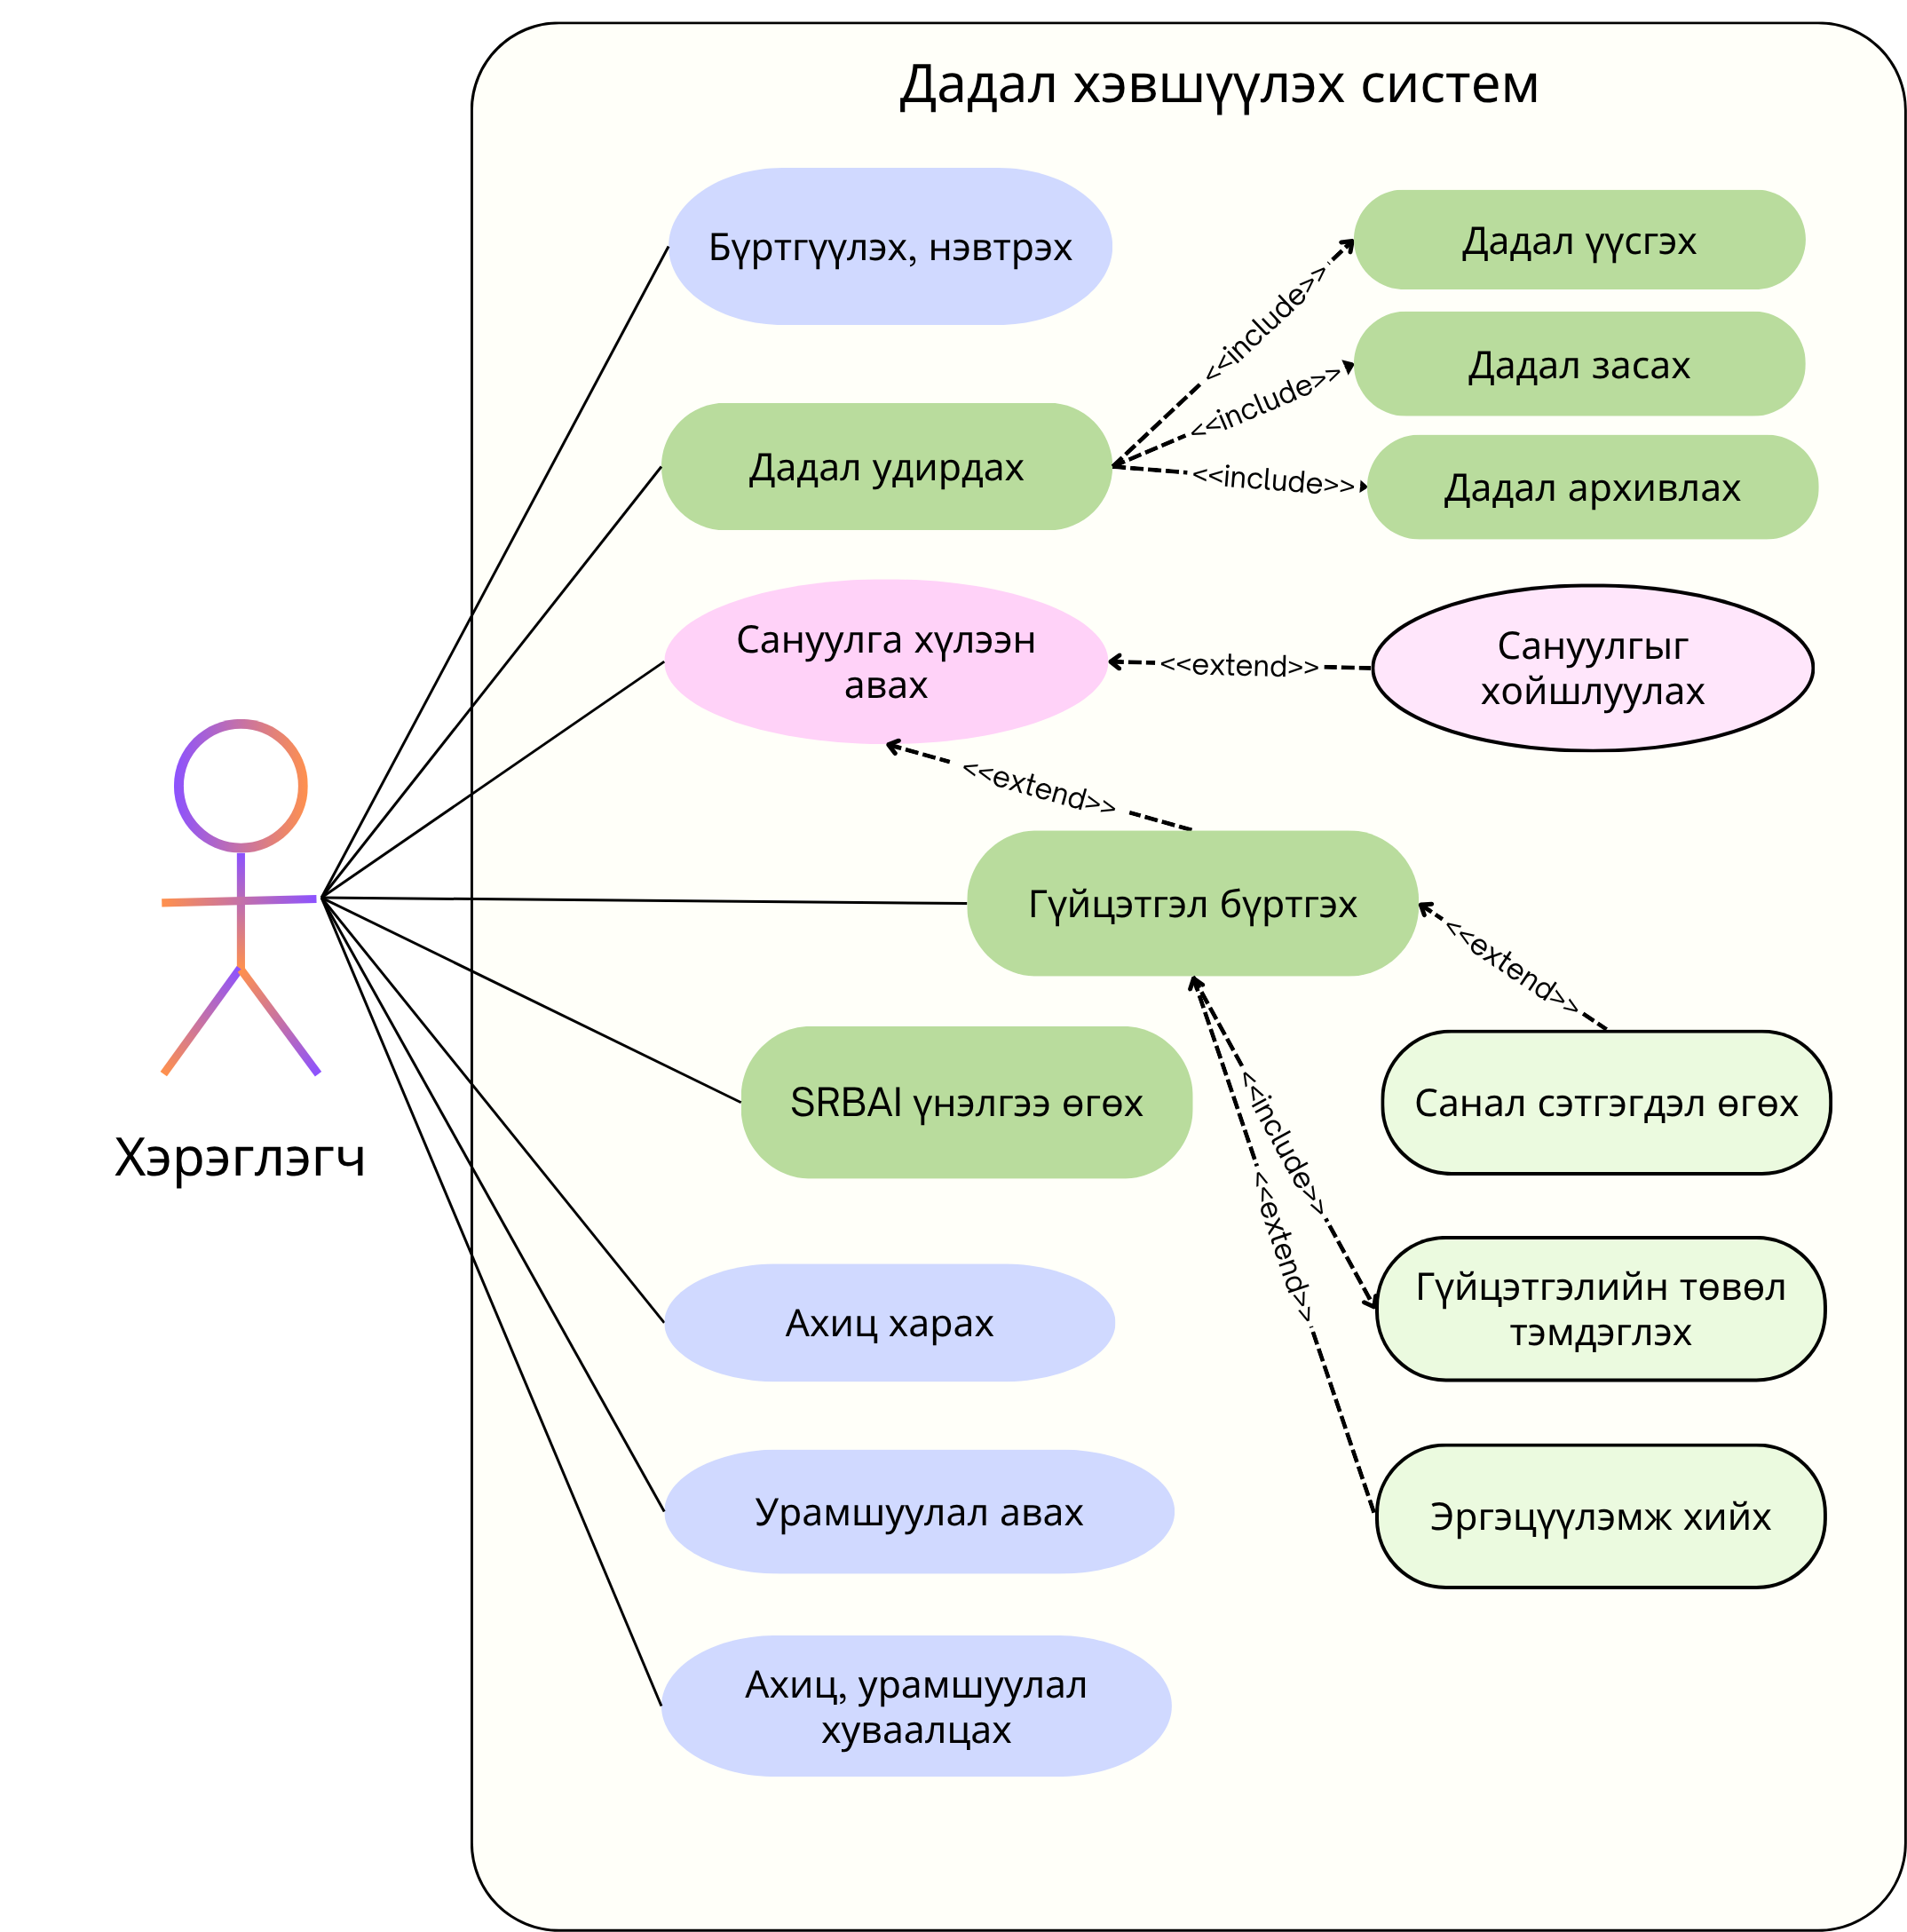
\includegraphics[width=0.72\textwidth]{images/GeneralUseCaseDiagram.png}
    \caption{Системийн ерөнхий хэрэглээний тохиолдлын диаграмм}
\end{figure}

\section{Системийн архитектурын зохиомж}

\subsection{Ерөнхий архитектур}

Туршилтын загварын архитектурыг хэрэгжүүлэх боломж, системийн төвөгшлийн түвшин, судалгааны ажлын цар хүрээг харгалзан клиент--сервер хэв маягтай, сервер талдаа модульчилсан нэг бүхэл архитектуртай, дотоод зохион байгуулалтын түвшинд цэвэр архитектурын зарчмыг баримталсан байдлаар зохиомжлов. Өөрөөр хэлбэл, систем нь байршуулалтын түвшинд нэг серверийн бүрэлдэхүүнтэй ажиллах боловч доторх логик нь үүргээрээ тусгаарлагдсан модулиудад хуваагдана.

Системийн хэрэглэгчийн тал нь React дээр хэрэгжсэн дэвшилтэт вэб програм (PWA) байна. Энэ нь веб болон хөдөлгөөнт орчинд ижил суурьтай хэрэглээний туршлага өгөхөөс гадна үйлчилгээний ажиллагчийн тусламжтайгаар вэб мэдэгдэл, хязгаарлагдмал оффлайн дэмжлэгийг хэрэгжүүлэх боломж бүрдүүлнэ. Сервер тал нь NestJS дээр хэрэгжих бөгөөд бүртгэл ба хандалт, дадлын удирдлага, өдөөгч нөхцөл ба хуваарь, сануулгын шийдвэрийн логик, гүйцэтгэл ба ахиц, санал сэтгэгдэл ба урамшуулал, дадал бэхжилтийн үнэлгээ, шинжилгээний модуль зэрэг үндсэн бүрэлдэхүүнүүдийг агуулна. Өгөгдлийн үндсэн сан нь PostgreSQL байх бөгөөд хуваарьт ажлын үйлчилгээ сануулгын дүрэмт логикийг хугацааны дагуу ажиллуулна.

Системийн ерөнхий архитектурын давхаргат зохион байгуулалтыг дараах зурагт үзүүлэв.

\begin{figure}[H]
    \centering
    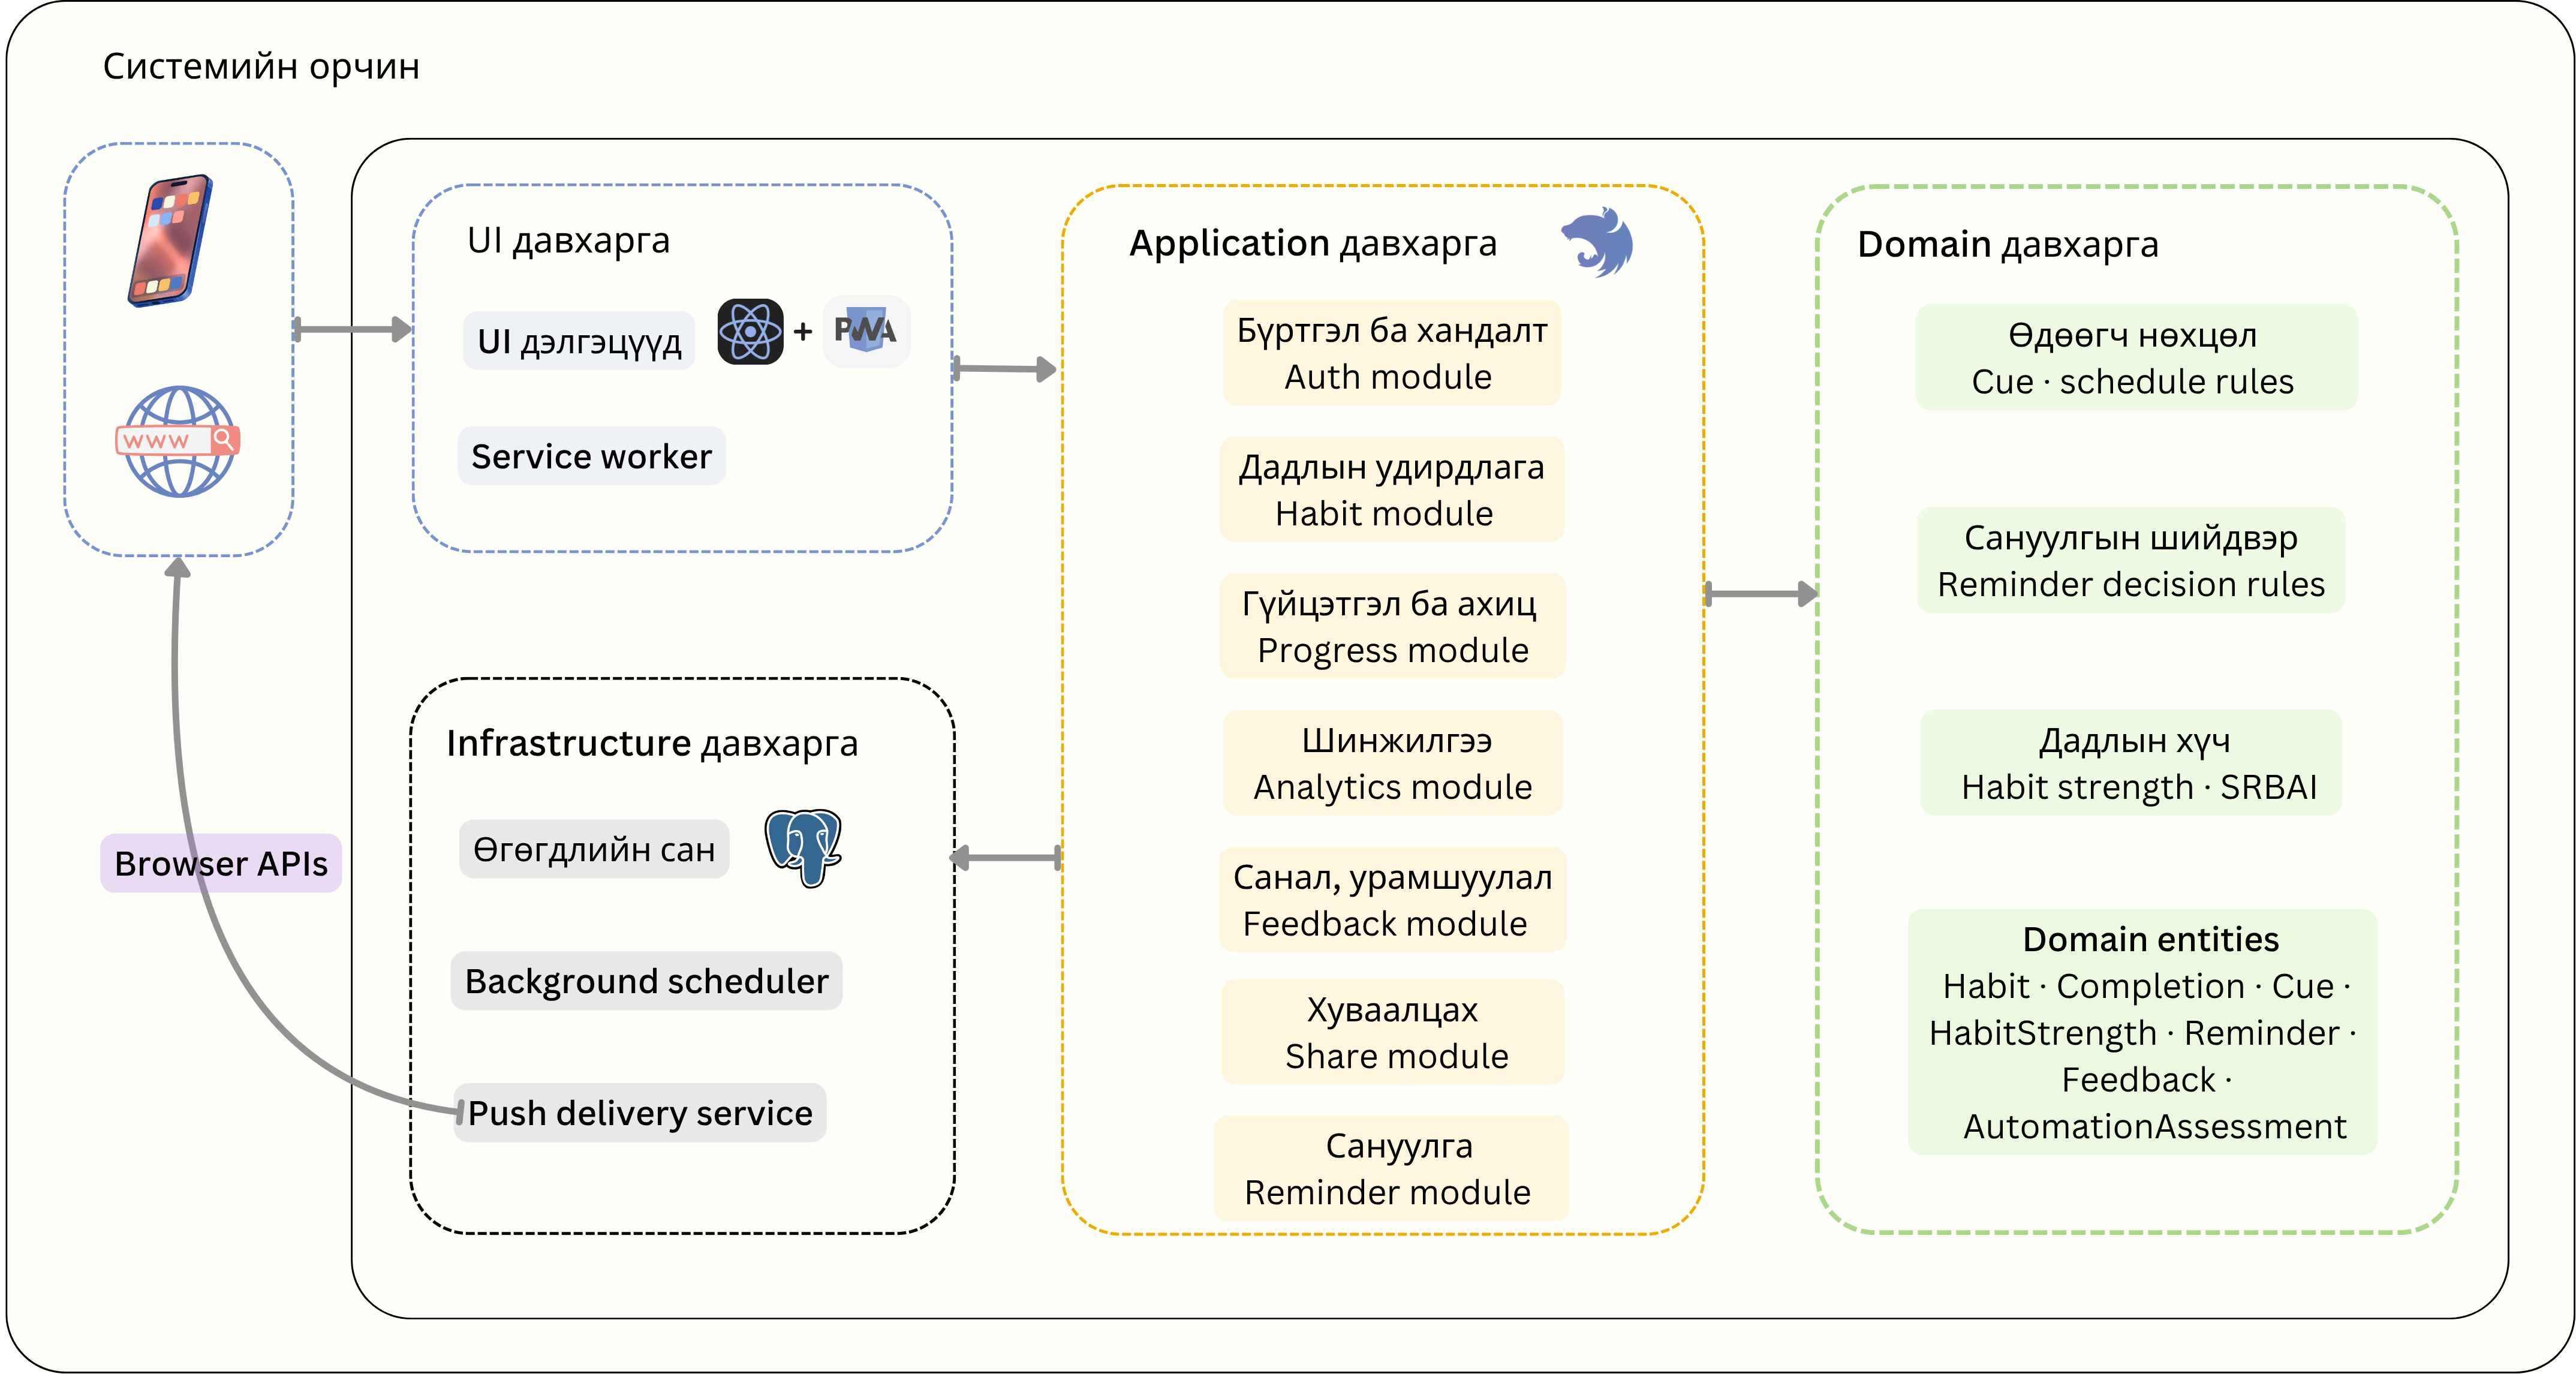
\includegraphics[width=0.96\textwidth]{images/CleanArchitectureDiagram.png}
    \caption{Системийн ерөнхий архитектур}
\end{figure}

\subsection{Архитектурын давхаргууд}

\begin{table}[htbp]
\centering
\small
\setlength{\tabcolsep}{4pt}
\begin{tabular}{|L{4.1cm}|L{8.9cm}|}
\hline
\textbf{Давхарга} & \textbf{Үндсэн үүрэг} \\
\hline
Хэрэглэгчийн интерфэйсийн түвшин & Дэлгэц, урсгал, компонент, хэрэглэгчийн шууд харилцан үйлчлэлийг хариуцах \\
\hline
Хэрэглээний логикийн түвшин & Модулиудын хэрэглээний урсгал, API, үйлчилгээний уялдаа холбоог хариуцах \\
\hline
Домайн логикийн түвшин & Системийн үндсэн дүрэм, хязгаарлалт, тооцооллын логикийг агуулна \\
\hline
Өгөгдөл ба дэд бүтцийн түвшин & Өгөгдөл хадгалах, гадаад үйлчилгээтэй холбогдох, мэдэгдэл хүргэх дэд бүтцийг хариуцна \\
\hline
\end{tabular}
\caption{Архитектурын давхаргууд}
\end{table}

\subsection{Хэрэглээний логикийн үндсэн модулиуд}

\begin{table}[htbp]
\centering
\small
\setlength{\tabcolsep}{4pt}
\begin{tabular}{|L{4.2cm}|L{8.8cm}|}
\hline
\textbf{Модуль} & \textbf{Үндсэн үүрэг} \\
\hline
Бүртгэл ба хандалтын модуль & Хэрэглэгчийн бүртгэл, нэвтрэлт, эрхийн шалгалтыг хариуцах \\
\hline
Дадлын удирдлагын модуль & Дадал үүсгэх, засах, архивлах, үндсэн шинжүүдийг удирдах \\
\hline
Өдөөгч нөхцөл ба хуваарийн модуль & Өдрийн цаг, өдрийн төрөл, нөхцөл байдал, хуваарийн мэдээллийг удирдах \\
\hline
Сануулгын модуль & Сануулга илгээх шаардлагатай эсэхийг дүрэмт логикоор шийдвэрлэх \\
\hline
Мэдэгдэл хүргэх модуль & Сануулгын мэдээллийг мэдэгдлийн дэд бүтцээр дамжуулан хүргэх \\
\hline
Гүйцэтгэл ба ахицын модуль & Гүйцэтгэл бүртгэх, цуваа тооцох, ахицын мэдээлэл гаргах \\
\hline
Санал сэтгэгдэл ба урамшууллын модуль & Санал сэтгэгдэл, урамшуулал, эргэцүүллийн мэдээллийг хариуцах \\
\hline
Дадлын хүчний модуль & Автоматжилтын үнэлгээ боловсруулах, нийлмэл оноо тооцоолох, бэхжилтийн түвшин үнэлэх \\
\hline
Шинжилгээний модуль & Хэрэглээний болон зан үйлийн үзүүлэлтүүдийг тооцоолох \\
\hline
Хуваалцах дэмжлэгийн модуль & Ахиц, урамшууллыг гадна орчинд хуваалцах урсгалыг дэмжих \\
\hline
\end{tabular}
\caption{Хэрэглээний логикийн үндсэн модулиуд}
\end{table}

Эдгээр модулиудын дундаас сануулгын модуль болон дадлын хүчний модуль нь уг системийн зан үйлийн дэмжлэгийн гол цөм болно. Сануулгын модуль нь өдөөгч нөхцөл, гүйцэтгэлийн түүх, сануулгад өгсөн үйлдлийн түүх, сануулгыг аажмаар бууруулах бодлого зэрэг мэдээлэлд тулгуурлан тухайн мөчид сануулга илгээх эсэхийг шийдвэрлэнэ. Харин дадлын хүчний модуль нь автоматжилтын үнэлгээ, гүйцэтгэлийн тогтвортой байдал, өдөөгч нөхцлийн тогтвортой байдал зэрэг мэдээлэлд тулгуурлан тухайн дадлын бэхжилтийн түвшнийг үнэлнэ. Модулиудын харилцан уялдаа нь дээр дурдсан ерөнхий архитектур болон хүснэгтэн тодорхойлолтуудад нэгтгэн тусгагдсан.

\subsection{Мэдэгдэл хүргэх механизм}

Архитектурын нэг чухал онцлог нь мэдэгдэл хүргэх логикийг хэрэглэгчийн интерфэйсээс тусад нь зохион байгуулсан явдал юм. Сануулгын модуль нь тухайн мөчид сануулга илгээх шаардлагатай гэж үзсэн тохиолдолд мэдэгдэл хүргэх бүрэлдэхүүнд мэдээлэл дамжуулна. Улмаар уг бүрэлдэхүүн нь вэб мэдэгдлийн дэд бүтцээр дамжуулан хэрэглэгчийн төхөөрөмж рүү сануулга илгээнэ.

Хэрэглэгчийн интерфэйс тухайн үед нээлттэй биш байсан ч үйлчилгээний ажиллагч мэдэгдлийг хүлээн авч, хөтөч эсвэл үйлдлийн системийн мэдэгдлийн орчинд харуулах боломжтой. Хэрэглэгч мэдэгдэл дээрээс шууд үйлдэл сонгосон тохиолдолд тухайн мэдээлэл сервер тал руу буцаж дамжин, сануулгын үйлдэл болон дараах гүйцэтгэлийн урсгалтай холбогдоно.

\section{Өгөгдлийн загварын зохиомж}

Системийн өгөгдлийн загвар нь дадал төлөвшлийн үйл явцыг зөвхөн ``хийсэн'' эсэхээр бус, харин ``ямар нөхцөлд'', ``ямар өдөөлтөөр'', ``ямар хариу үйлдэлтэйгээр'', ``ямар санал сэтгэгдэлтэйгээр'', мөн ``хэр зэрэг автоматжиж буй''-г системтэй хадгалах зорилготой. Үүний тулд дараах үндсэн өгөгдлийн нэгжүүдийг тодорхойлов.

\begin{table}[htbp]
\centering
\small
\setlength{\tabcolsep}{4pt}
\begin{tabular}{|L{4.6cm}|L{8.4cm}|}
\hline
\textbf{Өгөгдлийн нэгж} & \textbf{Тайлбар} \\
\hline
Хэрэглэгч & Системийн хэрэглэгчийн үндсэн мэдээлэл \\
\hline
Дадал & Хэрэглэгчийн хэрэгжүүлэх зан үйлийн үндсэн мэдээлэл, хуваарь, хэмжилтийн тохиргоог хадгална. \\
\hline
Шалтгаан & Тухайн дадлыг яагаад хэрэгжүүлэх гэж буй хувийн шалтгааны мэдээллийг хадгална. \\
\hline
Өдөөгч нөхцөл & Цагийн хүрээ, ерөнхий байршил, өмнөх үйлдэл зэрэг сануулгын шийдвэрт ашиглагдах нөхцөлийг хадгална. \\
\hline
Хуваарийн өдөр & Дадал аль өдрүүдэд идэвхтэй байхыг илэрхийлэх өгөгдөл \\
\hline
Жижиг алхам & Дадлыг хэрэгжүүлэхэд зориулсан жижиг алхмууд \\
\hline
Сануулга & Илгээсэн сануулгын бүртгэл \\
\hline
Сануулгын үйлдэл & Сануулгад өгсөн хэрэглэгчийн үйлдэл \\
\hline
\end{tabular}
\caption{Системийн үндсэн өгөгдлийн нэгжүүд (I)}
\end{table}

\begin{table}[htbp]
\centering
\small
\setlength{\tabcolsep}{4pt}
\begin{tabular}{|L{4.6cm}|L{8.4cm}|}
\hline
\textbf{Өгөгдлийн нэгж} & \textbf{Тайлбар} \\
\hline
Гүйцэтгэлийн бүртгэл & Бодит гүйцэтгэлийн утга, бүртгэсэн хугацаа, гүйцэтгэлийн эх үүсвэр, доод зорилт хангасан эсэх, үндсэн зорилт хүрсэн эсэхийг хадгална. \\
\hline
Хэцүү байдлын үнэлгээ & Гүйцэтгэлийн дараах төвөгшлийн үнэлгээг хадгална. \\
\hline
Эргэцүүлсэн санал сэтгэгдэл & Гүйцэтгэлийн дараах ашиг тусын талаарх товч эргэцүүллийг хадгална. \\
\hline
Автоматжилтын үнэлгээ & SRBAI-д суурилсан асуулгын хариулт, тооцоолсон оноо \\
\hline
Урамшууллын үйл явдал & Оноо, тэмдэг, баяр хүргэлт зэрэг урамшууллын бүртгэл \\
\hline
Дадлын хүч & Дадлын тогтворжилтын нийлмэл оноо, түвшний хадгалалт \\
\hline
Интерфэйсийн үйл явдлын бүртгэл & Микро түвшний хэрэглээний үйлдлийн бүртгэл \\
\hline
Хэрэглэгчийн үйл ажиллагааны бүртгэл & Апп нээх, ажиллагааны үе эхлүүлэх, ажиллагааны үе дуусгах зэрэг системийн ерөнхий хэрэглээний идэвхийг хадгална. \\
\hline
\end{tabular}
\caption{Системийн үндсэн өгөгдлийн нэгжүүд (II)}
\end{table}

Өгөгдлийн хамаарлын бүтэц дээр дадал нь төв нэгж болно. Нэг хэрэглэгч олон дадалтай байж болох бөгөөд дадал бүр нэг шалтгааны мэдээлэлтэй, олон өдөөгч нөхцөл, олон идэвхтэй өдөр, олон жижиг алхам, олон сануулга, олон гүйцэтгэлийн бүртгэлтэй холбогдоно. Гүйцэтгэлийн бүртгэл бүр нь хэцүү байдлын үнэлгээ, эргэцүүлсэн санал сэтгэгдэл, урамшууллын үйл явдалтай уялдах боломжтой. Мөн автоматжилтын үнэлгээ болон дадлын хүчний оноо нь хугацааны явцад олон удаа бүртгэгдэх тул тухайн дадлын өөрчлөлтийн чиг хандлалыг хугацааны дарааллаар шинжлэх боломж бүрдэнэ.

\section{Хэрэглэгчийн интерфэйс ба хэрэглээний туршлагын зохиомж}

Дадал үүсгэх дэлгэц нь хэрэглэгчээс олон салангид, төвөгтэй талбар бөглүүлэхийн оронд үндсэн гурван ойлголтыг төв болгон зохиомжилсон. Үүнд: юу хийх вэ, хэзээ эсвэл ямар нөхцөлд хийх вэ, яагаад хийх вэ гэсэн мэдээлэл орно. Систем нь эдгээр оролтод тулгуурлан хэрэглэгчид ойлгомжтой өгүүлбэрэн урьдчилсан харагдац үзүүлнэ. Жишээлбэл, ``Сэрснийхээ дараа би 5 минут бясалгал хийнэ. Шалтгаан: өдрийг тайван эхлүүлэхийн тулд.'' гэсэн хэлбэрийн урьдчилсан харагдац нь хэрэглэгчийн оруулсан мэдээллийг нэг мөр ойлгож, баталгаажуулахад дэмжлэг үзүүлнэ. Ийнхүү интерфэйс нь өгөгдлийг бүтцэт байдлаар хадгалж байгаа боловч хэрэглэгчид байгалийн хэллэгт ойр, ойлгомжтой хэлбэрээр харуулах зарчмыг баримтална.

\section{Системийн ажиллагааны үндсэн логик}

\providecommand{\systemdiagram}[2]{%
\begin{figure}[H]
    \centering
    \includegraphics[width=\textwidth,height=0.82\textheight,keepaspectratio]{#1}
    \caption{#2}
\end{figure}
}

Системийн ажиллагааны үндсэн логик нь дадал төлөвшлийн мөчлөгийн дараалалтай нийцсэн байдлаар зохион байгуулагдсан. Өөрөөр хэлбэл, систем нь хэрэглэгчийн зан үйлийг зөвхөн бүртгэх бус, харин эхлүүлэх, хэрэгжүүлэх, бататгах, аажмаар тогтворжуулах чиглэлээр дэмжинэ.

\subsection{Үндсэн урсгал}

Системийн ажиллагааны үндсэн урсгал дараах байдалтай байна. Нэгдүгээрт, хэрэглэгч шинэ дадал үүсгэж, түүнд хамаарах зорилго, өдөөгч нөхцөл, хуваарь, шаардлагатай бол жижиг алхмуудыг тохируулна. Хоёрдугаарт, систем эдгээр мэдээлэлд тулгуурлан сануулгын логикийг бэлтгэнэ. Гуравдугаарт, тохирох нөхцөл бүрдсэн үед сануулгын модуль сануулга илгээх эсэхийг шийдвэрлэж, шаардлагатай бол мэдэгдэл хүргэх модуль рүү дамжуулна. Дөрөвдүгээрт, хэрэглэгч сануулгад үйлдэл сонгож, эсвэл өөрийн санаачилгаар гүйцэтгэл бүртгэнэ. Тавдугаарт, гүйцэтгэлийн дараа урамшуулал, санал сэтгэгдэл, эргэцүүллийн урсгал идэвхжинэ. Зургаадугаарт, систем хуримтлагдсан өгөгдөлд тулгуурлан ахиц, цуваа, автоматжилтын түвшин, дадлын хүчний оноо, сануулгаас хараат бус байдлын үзүүлэлтийг тооцоолно. Долоодугаарт, дадал тогтворжихын хэрээр сануулгын давтамжийг аажмаар бууруулж, хэрэглэгчийн өөрийн санаачилгатай зан үйлийг дэмжинэ.

Системийн үндсэн ажиллагааны дарааллыг дээрх урсгалын тайлбарт үе шат бүрээр нь нэгтгэн үзүүлэв.

\noindent Үндсэн системийн урсгалын үйл ажиллагааны диаграмм.
Энэхүү үйл ажиллагааны диаграмм нь системийн ерөнхий урсгалыг хэрэглэгчийн дадал үүсгэхээс эхлэн сануулга, гүйцэтгэл бүртгэл, санал сэтгэгдэл, ахицын тооцоолол, сануулгын бодлогын шинэчлэлт хүртэлх дарааллаар үзүүлж байна.

\systemdiagram{images/ActivityDiagram1.png}{Дадал төлөвшүүлэх системийн үндсэн үйл ажиллагааны урсгал}

Дадал үүсгэх, тохируулах, хадгалах дарааллын нарийвчилсан харилцан үйлчлэлийн диаграммыг хавсралтад үзүүлэв.

\subsection{Дадал төлөвшлийн мөчлөг ба системийн хэрэгжилтийн уялдаа}

\begin{table}[htbp]
\centering
\small
\setlength{\tabcolsep}{4pt}
\begin{tabular}{|L{4.8cm}|L{8.2cm}|}
\hline
\textbf{Дадал төлөвшлийн мөчлөгийн үе шат} & \textbf{Системийн хэрэгжилт} \\
\hline
Өдөөгч дохио & Нөхцөл байдалд суурилсан сануулга, өдөөгч нөхцлийн тохиргоо, сануулгын тайлбар \\
\hline
Хүсэл тэмүүлэл & Хувийн шалтгаан, зорилгын утгыг эргэн сануулах мэдээлэл \\
\hline
Хариу үйлдэл & ``Хийсэн'', ``хэсэгчлэн хийсэн'' бүртгэл, нэг товшилтын урсгал, жижиг алхам, хялбаршуулах дэмжлэг \\
\hline
Урамшуулал & Оноо, баяр хүргэлт, тасралтгүй гүйцэтгэлийн цуваа, эргэцүүлсэн санал сэтгэгдэл \\
\hline
Бэхжилт ба автоматжилт & SRBAI үнэлгээ, дадлын хүчний оноо, сануулгын бодлогын өөрчлөлт \\
\hline
\end{tabular}
\caption{Дадал төлөвшлийн мөчлөг ба системийн хэрэгжилтийн уялдаа}
\end{table}

Энэхүү уялдаа нь онолын загвар системийн функц, өгөгдлийн бүтэц, харилцан үйлчлэлийн урсгалын түвшинд бодитоор тусгагдсан болохыг харуулна.

\subsection{Сануулгаас хараат бус байдлыг хянах логик}

Уг системийн ялгарах нэг онцлог нь гүйцэтгэлийн эх үүсвэрийг ангилан бүртгэх явдал юм. Өөрөөр хэлбэл, хэрэглэгчийн гүйцэтгэл сануулгын шууд нөлөөгөөр хийгдсэн үү, эсвэл хэрэглэгч өөрийн санаачилгаар хийсэн үү гэдгийг ялган хадгална. Үүний тулд гүйцэтгэлийн бүртгэл бүр дээр эх үүсвэрийн ангилал хадгална. Үүнд сануулгад тулгуурласан, өөрийн санаачилгатай, тодорхойгүй гэсэн ангиллууд орно.

Хэрэв хэрэглэгч сануулгад үйлдэл сонгосны дараа богино хугацаанд гүйцэтгэл бүртгэсэн бол тухайн үйлдлийг сануулгад тулгуурласан гэж ангилна. Харин хэрэглэгч сануулгагүй үед системийг өөрөө нээн гүйцэтгэл бүртгэсэн бол өөрийн санаачилгатай гэж ангилна. Энэ ангилал нь сануулгаас хэт хараат байдлыг үнэлэх, дадал аажмаар дотооджиж байгаа эсэхийг шинжлэх суурь өгөгдөл болно.

Сануулгыг нөхцөл байдалд тулгуурлан шийдвэрлэх дүрэмт логик нь өдрийн идэвхтэй хуваарь, цагийн хүрээ, өмнөх гүйцэтгэл, хүлээлгийн хугацаа болон сануулгын бодлогын нөхцөлийг хамтатган авч үздэг. Энэ урсгалын үйл ажиллагааны болон дарааллын дэлгэрэнгүй диаграммуудыг хавсралтад оруулав.

\begin{table}[htbp]
\centering
\small
\setlength{\tabcolsep}{4pt}
\begin{tabular}{|L{6.5cm}|L{6.5cm}|}
\hline
\textbf{Нөхцөл} & \textbf{Ангиллын шийдвэр} \\
\hline
Хэрэглэгч сануулгад үйлдэл сонгосны дараа богино хугацаанд гүйцэтгэл бүртгэсэн & Сануулгад тулгуурласан гүйцэтгэл \\
\hline
Хэрэглэгч сануулгагүйгээр системийг өөрөө нээж гүйцэтгэл бүртгэсэн & Өөрийн санаачилгатай гүйцэтгэл \\
\hline
Эх үүсвэрийг тодорхой ялгах боломжгүй & Тодорхойгүй эх үүсвэр \\
\hline
\end{tabular}
\caption{Гүйцэтгэлийн эх үүсвэрийн ангилал}
\end{table}

Дээрх ангилал нь хэрэглэгчийн зан үйл сануулгад хэр зэрэг түшиглэж байгаа, эсвэл аажмаар төлөвшиж байгаа эсэхийг шинжлэх үндсэн суурь өгөгдөл болно.

Өөрийн санаачилгатай бүртгэл, сануулгад хариулах урсгал, мөн гүйцэтгэлээс урамшуулал хүртэлх нарийвчилсан диаграммуудыг хавсралтад тусгав.

\subsection{Сануулгыг аажмаар бууруулах ба дасан зохицох логик}

Систем нь хэрэглэгчийг үргэлж ижил түвшний сануулгаар өдөөх бус, дадал тогтворжихын хэрээр сануулгын давтамжийг аажмаар бууруулах логиктой байна. Үүнийг сануулгыг аажмаар бууруулах бодлого гэж үзнэ. Энэ бодлого нь дадлын хүчний оноо, автоматжилтын түвшин, гүйцэтгэлийн тогтвортой байдал, сануулгагүй нөхцөл дэх гүйцэтгэл, өдөөгч нөхцлийн тогтвортой байдал зэрэг үзүүлэлтэд тулгуурлана.

Үүний зэрэгцээ, гүйцэтгэлийн хувь сулрах, хэцүү байдлын үнэлгээ өндөр гарах, сануулгад сөрөг үйлдэл давтагдах, эсвэл автоматжилтын өсөлт саарах зэрэг нөхцөлд систем дасан зохицох дэмжлэг үзүүлнэ. Ийм дэмжлэг нь дадлыг жижиг алхамд хуваах, зорилтот утгыг бууруулах, сануулгын цагийн хүрээг өөрчлөх, өдөөгч нөхцлийг илүү бодитой болгох, хамгийн бага хувилбар санал болгох зэрэг зөвлөмжийн хэлбэртэй байна.

Дадлын хүчийг дахин үнэлэх, сануулгын бодлого шинэчлэх, дасан зохицох санал гаргах урсгал нь системийн дасан зохицох шийдвэрийн гол хэсэг юм. Энэ логикийн дэлгэрэнгүй үйл ажиллагааны болон дарааллын диаграммыг хавсралтад үзүүлэв.

Энэхүү логик нь системийн зорилго зөвхөн сануулахад бус, харин хэрэглэгчийн амжилттай гүйцэтгэж чадах боломжит нөхцөлийг бүрдүүлэхэд оршиж байгааг илэрхийлнэ.

\section{Амжилтын шалгуур ба хэмжигдэх үзүүлэлт}

\subsection{Амжилтын шалгуур}

Амжилтын шалгуур нь туршилтын загвар шаардлагын түвшинд хангалттай хэрэгжсэн эсэхийг үнэлэхэд ашиглагдана.

\begin{table}[htbp]
\centering
\footnotesize
\setlength{\tabcolsep}{3pt}
\begin{tabular}{|L{1.4cm}|L{6.6cm}|L{4.3cm}|}
\hline
\textbf{Код} & \textbf{Амжилтын шалгуур} & \textbf{Үнэлэх арга} \\
\hline
АШ-01 & Хэрэглэгч дадлаа хуваарь, зорилтот утга, өдөөгч нөхцөл, шалтгааны мэдээлэлтэй нь бүрэн үүсгэж чаддаг байх & Дадал үүсгэх урсгалын хүлээн зөвшөөрөх туршилт \\
\hline
АШ-02 & Систем сануулга үүсгэж, илгээж, хэрэглэгчийн үйлдлийг бүрэн бүртгэдэг байх & Сануулгын ажлын урсгалын туршилт \\
\hline
АШ-03 & Хэрэглэгч гүйцэтгэлийг төвөгшил багатай бүртгэж чаддаг байх & Хурдан бүртгэлийн хэрэглэгчийн урсгалын туршилт \\
\hline
АШ-04 & Систем жижиг алхам, хэцүү байдлын үнэлгээ, санал сэтгэгдлийг зөв хадгалдаг байх & Өгөгдөл хадгалалтын туршилт \\
\hline
АШ-05 & Систем автоматжилтын үнэлгээ, цуваа, урамшуулал, дадлын хүчний оноог зөв тооцоолдог байх & Урьдчилан бэлтгэсэн өгөгдлөөр баталгаажуулах \\
\hline
АШ-06 & Систем ахицын шинжилгээ болон түүхийг ойлгомжтой харуулдаг байх & Хяналтын самбарын хүлээн зөвшөөрөх туршилт \\
\hline
АШ-07 & Систем судалгааны үзүүлэлтүүдийг тооцоход хангалттай өгөгдөл цуглуулдаг байх & Үзүүлэлт гаргалтын туршилт \\
\hline
АШ-08 & Хэрэглэгч урамшуулал эсвэл ахицын мэдээллээ хуваалцаж чаддаг байх & Хуваалцах урсгалын туршилт \\
\hline
\end{tabular}
\caption{Туршилтын загварын амжилтын шалгуур}
\end{table}

\subsection{Хэмжигдэх үндсэн үзүүлэлтүүд}

Энэ судалгаанд системийн хэрэглээ, үр нөлөө, зан үйлийн тогтворжилтыг үнэлэх зорилгоор дараах үндсэн үзүүлэлтүүдийг ашиглана.

\begin{table}[htbp]
\centering
\small
\setlength{\tabcolsep}{4pt}
\begin{tabular}{|L{4.0cm}|L{9.0cm}|}
\hline
\textbf{Үзүүлэлтийн бүлэг} & \textbf{Хэмжигдэх үндсэн үзүүлэлтүүд} \\
\hline
Өдөөгч дохио ба сануулга & Өдөөгч нөхцөл тохируулсан хувь, сануулга нээсэн хувь, сануулгад үйлдэл сонгосон хувь, сануулгын үйлдлийн тархалт, сануулгын цаг тохиромжтой байсан хувь, сануулгын давтамжийн өөрчлөлт \\
\hline
Сэдэл ба эргэцүүлэл & Шалтгааны мэдээлэл оруулсан хувь, шалтгааны мэдээлэлтэй холбоотой сануулга эсвэл тайлбар үзсэн хувь, эргэцүүлэл бөглөсөн хувь, зорилготой нийцэж буй субъектив үнэлгээ \\
\hline
Гүйцэтгэл ба төвөгшил & Нийт гүйцэтгэлийн хувь, хэсэгчлэн гүйцэтгэлийн хувь, гүйцэтгэл бүртгэхэд зарцуулсан хугацаа, жижиг алхмын гүйцэтгэлийн хувь, хэцүү байдлын оноо, хялбаршуулах санал хүлээн авсан хувь \\
\hline
Тогтворжилт ба дотооджилт & Сануулгагүй нөхцөл дэх гүйцэтгэлийн хувь, тасралтгүй гүйцэтгэлийн цувааны урт, сэргээх боломж ашигласан хувь, автоматжилтын оноо, дадлын хүчний оноо, сануулгаас хэт хараат байдлын үзүүлэлт \\
\hline
Хэрэглээ ба оролцоо & 1, 7, 30 дахь өдрийн эргэн ирэлтийн үзүүлэлт, ахицын өөрчлөлтийн чиг хандлага, хуваалцах үйлдлийн хувь \\
\hline
\end{tabular}
\caption{Хэмжигдэх үндсэн үзүүлэлтүүд}
\end{table}

Эдгээр үзүүлэлт нь зөвхөн систем ашиглагдсан эсэхийг бус, мөн тухайн систем хэрэглэгчийн зан үйлийн тогтворжилтод ямар нөлөө үзүүлж байгааг үнэлэх боломж олгоно.

\section{Системийн хязгаарлалт}

Туршилтын загварыг дэвшилтэт вэб програм хэлбэрээр хэрэгжүүлж байгаа тул дараах хязгаарлалтыг харгалзан үзэв. Нэгдүгээрт, систем нь төхөөрөмжийн дэлгэцийн төлөв, төхөөрөмжийн түвшний хэрэглээний түүх, түгжээтэй дэлгэцийн тусгай удирдлага зэрэг доод түвшний мэдээлэлд тогтвортой хандах боломжгүй. Хоёрдугаарт, вэб мэдэгдлийн дэмжлэг болон мэдэгдлийн үйлдлийн товчлууруудын ажиллагаа нь хөтөч болон үйлдлийн системээс хамааран ялгаатай байж болно. Гуравдугаарт, байршлын мэдээллийг зөвхөн ерөнхий ангиллын түвшинд авч үзэх бөгөөд өндөр нарийвчлалтай байнгын хяналт хийхгүй. Дөрөвдүгээрт, сануулгын шийдвэрийн логик нь дүрэмт зарчимд суурилсан бөгөөд машин сургалтын таамаглалын хөдөлгүүр хэрэгжүүлэхгүй. Тавдугаарт, дадлын хүчний оноо нь туршилтын загварт зориулсан үйл ажиллагааны загвар тул сэтгэлзүйн баталгаажсан стандарттай ижил түвшний хэмжүүр гэж үзэхгүй.

\section{Бүлгийн дүгнэлт}

Уг бүлэгт зан үйлд суурилсан дадал төлөвшүүлэх системийн зорилтот хэрэглэгчийн бүлэг, хэрэглэгчийн үүрэг, хамрах хүрээ, функциональ болон функциональ бус шаардлага, хэрэглээний тохиолдол, архитектурын зохиомж, өгөгдлийн загвар, үндсэн ажиллагааны логик, амжилтын шалгуур, хэмжигдэх үзүүлэлт, мөн туршилтын загварын хязгаарлалтыг системтэйгээр тодорхойлов.

Ингэснээр өмнөх бүлгүүдэд авч үзсэн онолын ойлголтуудыг системийн түвшинд хэрэгжихүйц хэлбэрт хөрвүүлсэн болно. Тухайлбал, өдөөгч дохио, сэдэл, хариу үйлдэл, урамшуулал, автоматжилт зэрэг зан үйлийн үндсэн ойлголтуудыг сануулгын логик, шалтгааны мэдээлэл, гүйцэтгэлийн бүртгэл, санал сэтгэгдэл, урамшууллын механизм, автоматжилтын үнэлгээ, дадлын хүчний оноо зэрэг програм хангамжийн бүрэлдэхүүнтэй уялдуулан зохиомжлов.

Мөн системийг клиент--сервер хэв маягтай, модульчилсан нэг бүхэл архитектуртай, цэвэр архитектурын зарчимд нийцүүлэн төлөвлөснөөр туршилтын загварын түвшинд хэрэгжүүлэх боломж, логикийн цэгцтэй байдал, цаашид өргөтгөх нөхцөлийг хангаж байна. Иймээс энэхүү бүлэг нь дараагийн хэрэгжүүлэлт, интерфэйсийн зохиомж, туршилт, үнэлгээний ажлын шууд суурь болно.



\chapter{ТУРШИЛТ БА ҮНЭЛГЭЭ}

\section{Үнэлгээний зорилго}

Энэ бүлэгт зан үйлд суурилсан дадал төлөвшүүлэх системийг бодит хэрэглэгчдээр туршуулсан үр дүнг нэгтгэн үнэлэв. Үнэлгээний зорилго нь системийн хэрэглээнд тохиромжтой байдал, дадал үүсгэх болон гүйцэтгэл бүртгэх урсгалын ойлгомжтой байдал, сануулгын хэрэгцээ, ахиц болон дадлын хүчний мэдээллийн ашиг тус, хэрэглэгчийн сэтгэл ханамжийг тодорхойлох явдал байв.

Мөн системийн цөм санаа болох өдөөгч нөхцөлд суурилсан дадал төлөвшүүлэлт, доод зорилт, төхөөрөмжийн мэдэгдэл, гүйцэтгэлийн бүртгэл, SRBAI-д тулгуурласан дадлын хүчний оноо, дасан зохицох зөвлөмж зэрэг боломжууд өдөр тутмын хэрэглээнд хэр ойлгомжтой, хэрэгтэй байгааг шалгахыг зорьсон.

\section{Судалгааны зохиомж}

Үнэлгээнд холимог арга зүйт, нэг бүлэгт суурилсан хэрэглэгчийн туршилтын зохиомж ашиглав. Оролцогчид системийг өөрийн сонгосон дадал дээр ашиглаж, туршилтын төгсгөлд Google Forms-оор судалгааны асуулгад хариулсан. Ингэснээр системийн дотоод бүртгэлийн өгөгдөл, хэрэглэгчийн өөрийн үнэлгээ, санал сэтгэгдлийг хамтатган авч үзэх боломж бүрдсэн.

Судалгаанд нийт 20 хэрэглэгч оролцсон. Оролцогчид системд бүртгүүлж, дор хаяж нэг дадал үүсгэн, хуваарь, цагийн хүрээ, өдөөгч нөхцөл, сануулга болон зорилтот хэмжилтийн мэдээллээ тохируулсан. Туршилтын явцад тэд гүйцэтгэлээ бүртгэх, сануулгад хариу өгөх, ахицын мэдээллээ харах, санал хүсэлт илгээх боломжтой байв.

\section{Оролцогчид}

Оролцогчдыг дадал төлөвшүүлэх хэрэгцээ өндөртэй зорилтот бүлгээс сонгосон. Үүнд их, дээд сургуулийн оюутан, залуу ажиллагч, өдөр тутмын хичээл, ажил, эрүүл мэнд, бүтээмжийн дадлаа тогтмол болгох сонирхолтой хэрэглэгчид багтсан. Оролцогч бүр өөрт хэрэгтэй гэж үзсэн дадлыг сонгосон тул бүртгэгдсэн дадлууд нь дасгал хөдөлгөөн, ус уух, унших, хичээл хийх, эрт унтах, хувийн бүтээмжийн жижиг үйлдэл зэрэг төрөл бүрийн чиглэлтэй байв.

\section{Туршилтын явц}

Туршилтыг дараах үндсэн үе шаттайгаар зохион байгуулсан.

\begin{enumerate}
    \item \textbf{Танилцуулга ба бүртгэл:} Оролцогчдод системийн зорилго, үндсэн боломжуудыг тайлбарлаж, бүртгэл болон нэвтрэх урсгалыг ашиглуулсан.
    \item \textbf{Дадал үүсгэх:} Хэрэглэгч бүр дадлын нэр, хэмжилтийн төрөл, доод зорилт, хуваарь, өдөөгч нөхцөл, цагийн хүрээ, сануулгын тохиргоог бөглөсөн.
    \item \textbf{Өдөр тутмын хэрэглээ:} Оролцогчид дадлаа гүйцэтгэх үедээ системд бүртгэл хийж, сануулга ирсэн тохиолдолд ``хийсэн'' эсвэл ``хойшлуулах'' үйлдэл ашигласан.
    \item \textbf{Ахиц ба зөвлөмж харах:} Хэрэглэгчид үндсэн, дадлын дэлгэрэнгүй, ахицын шинжилгээ, профайл дэлгэцүүдээр дамжуулан ахиц, дараалал, дадлын хүч, амжилт, зөвлөмжийн мэдээлэлтэй харилцсан.
    \item \textbf{Эцсийн судалгаа:} Туршилтын дараа хэрэглэгчид профайл хэсэгт байршуулсан Google Forms холбоосоор ашиглахад хялбар байдал, үр ашиг, сануулгын тохиромжтой байдал, сайжруулах саналын талаар хариулт өгсөн.
\end{enumerate}

\section{Цуглуулсан өгөгдөл}

Үнэлгээнд ашигласан өгөгдлийг хоёр үндсэн бүлэгт хуваав. Нэгдүгээрт, системийн ажиллагаанаас автоматаар үүсэх тоон өгөгдөл; хоёрдугаарт, хэрэглэгчийн өөрийн үнэлгээ болон чөлөөт санал сэтгэгдэл юм.

\begin{table}[htbp]
\centering
\small
\setlength{\tabcolsep}{4pt}
\begin{tabular}{|p{4.0cm}|p{8.8cm}|}
\hline
\textbf{Өгөгдлийн төрөл} & \textbf{Тайлбар} \\ \hline
Гүйцэтгэлийн бүртгэл & Дадал хийсэн эсэх, бодит утга, бүртгэсэн хугацаа, доод зорилт болон үндсэн зорилтын биелэлт \\ \hline
Сануулгын өгөгдөл & Илгээсэн сануулга, хийсэн/хойшлуулах үйлдэл, сануулгын хугацаа, холбогдсон сануулгын мэдээлэл \\ \hline
Өдөөгч нөхцөл ба нөхцөл байдлын өгөгдөл & Цагийн хүрээ, байршил, өмнөх үйлдэл, тухайн нөхцөлд гүйцэтгэсэн эсэх \\ \hline
Дадлын хүчний өгөгдөл & SRBAI үнэлгээ, тогтвортой байдал, нөхцөл байдлын тогтвортой байдал, нийлмэл дадлын хүчний оноо \\ \hline
Оролцооны өгөгдөл & XP, амжилтын тэмдэг, дараалал, профайл болон ахицын шинжилгээний дэлгэцийн хэрэглээ \\ \hline
Судалгааны өгөгдөл & Ашиглахад хялбар байдал, сэтгэл ханамж, сануулгын үр нөлөө, сайжруулах санал \\ \hline
\end{tabular}
\caption{Үнэлгээнд ашигласан өгөгдлийн төрлүүд}
\label{tab:evaluation-data-types}
\end{table}

\section{Үнэлгээний шалгуур үзүүлэлтүүд}

Системийг дараах шалгуур үзүүлэлтээр үнэлэв.

\begin{itemize}
    \item \textbf{Хэрэглээний ойлгомжтой байдал:} бүртгэл, дадал үүсгэх, гүйцэтгэл бүртгэх урсгал хэрэглэгчид ойлгомжтой эсэх;
    \item \textbf{Дадал төлөвшүүлэх дэмжлэг:} өдөөгч нөхцөл, доод зорилт, сануулга, шалтгаан, алхам зэрэг тохиргоо нь дадлаа хэрэгжүүлэхэд тусалсан эсэх;
    \item \textbf{Сануулгын тохиромжтой байдал:} төхөөрөмжийн мэдэгдэл зөв цагт, хэрэгтэй мэдээлэлтэй ирсэн эсэх;
    \item \textbf{Ахицын мэдээллийн хэрэгцээ:} үндсэн, ахицын шинжилгээ, дадлын дэлгэрэнгүй дэлгэцүүдийн мэдээлэл хэрэглэгчид өөрийн явцыг ойлгоход тусалсан эсэх;
    \item \textbf{Урамшууллын нөлөө:} XP, амжилтын тэмдэг, дараалал, амжилтын мэдээлэл нь хэрэглэгчийн үргэлжлүүлэх сэдэлд эерэг нөлөөтэй эсэх;
    \item \textbf{Системийн ерөнхий сэтгэл ханамж:} хэрэглэгчид цаашид үргэлжлүүлэн ашиглах хүсэлтэй эсэх.
\end{itemize}

\section{Судалгааны үр дүн}

\subsection{Ашиглахад хялбар байдал}

Судалгааны хариултаас харахад хэрэглэгчид бүртгүүлэх, дадал үүсгэх, тухайн өдрийн дадлаа харах, гүйцэтгэл бүртгэх урсгалыг ерөнхийдөө ойлгомжтой гэж үнэлсэн. Ялангуяа үндсэн дэлгэц дээр өдрийн дадлууд нэг дор харагдах, дадлын картаас шууд гүйцэтгэл бүртгэх боломж нь өдөр тутмын хэрэглээнд тохиромжтой гэж үзэгдсэн.

Дадал үүсгэх маягт нь олон тохиргоотой боловч өгүүлбэрэн бүтэцтэй зохион байгуулагдсан. Энэ нь хэрэглэгчид ``юу хийх'', ``хэзээ хийх'', ``ямар нөхцөлд хийх'', ``яагаад хийх'' гэсэн асуултаар дадлаа тодорхойлоход тусалсан. Гэсэн хэдий ч зарим хэрэглэгч анх удаа ашиглах үед нэмэлт заавар хэрэгтэй гэж санал өгсөн. Иймээс эхний танилцуулга болон товч тусламжийн тайлбарыг цаашид нэмэгдүүлэх шаардлагатай.

\subsection{Өдөөгч нөхцөл болон сануулгын үр нөлөө}

Оролцогчдын саналд цагийн хүрээ, өмнөх үйлдэл, төхөөрөмжийн мэдэгдэл зэрэг боломжууд дадлаа марталгүй хийхэд тусалсан гэж давтагдан дурдагдсан. Ялангуяа ``өглөө'', ``хичээлийн дараа'', ``унтахын өмнө'' гэх мэт өдөр тутмын тогтсон нөхцөлтэй холбож дадал үүсгэх нь бодит амьдралын хуваарьтайгаа уялдуулахад дөхөм байв.

Сануулгын хувьд ``хийсэн'' болон ``хойшлуулах'' гэсэн хоёр үйлдэл хангалттай энгийн байсан. Хийсэн үйлдэл нь сануулгатай холбоотой гүйцэтгэлийг автоматаар бүртгэх тул хэрэглэгчээс нэмэлт алхам шаардахгүй. Харин хойшлуулах үйлдэл нь тухайн үед хийх боломжгүй боловч бүр мөсөн мартахгүй байх хэрэгцээг хангаж байна. Үүнээс үзэхэд сануулгыг зөвхөн мэдэгдэл илгээх бус, хэрэглэгчийн нөхцөл байдалд тохирсон богино үйлдэлтэй холбох нь хэрэглээний үр ашгийг нэмэгдүүлсэн.

\subsection{Ахицын шинжилгээ ба дадлын хүчний мэдээлэл}

Үндсэн болон дадлын дэлгэрэнгүй дэлгэцүүд дээр дараалал, хуанли, гүйцэтгэлийн түүх, цагийн хүрээ, өдөөгч нөхцөл, шалтгаан зэрэг мэдээллийг нэг дор харуулсан нь хэрэглэгчид өөрийн дадлын явцыг ойлгоход тусалсан. Ахицын шинжилгээний хуанли болон идэвхийн дүрслэл нь аль өдрүүдэд тогтвортой байсан, аль үед тасалдсан гэдгийг харахад хэрэгтэй гэж үнэлэгдсэн.

Дадлын хүчний оноо нь SRBAI, гүйцэтгэлийн тогтвортой байдал, нөхцөл байдлын тогтвортой байдал гэсэн гурван бүрэлдэхүүнтэй. Тиймээс зөвхөн ``хийсэн тоо''-гоор бус, дадал автоматжиж байгаа эсэхийг илүү өргөн өнцгөөс тайлбарлах боломж өгсөн. Хэрэглэгчийн хувьд энэ оноо нь өөрийн ахицыг нэг тоон үзүүлэлтээр харах давуу талтай боловч бүрэлдэхүүн хэсгүүдийг илүү энгийн хэлээр тайлбарлах хэрэгцээ ажиглагдсан.

\subsection{Урамшуулал, XP ба амжилтын тэмдэг}

Профайл хэсэгт XP, амжилтын тэмдэг, амжилтын мэдээллийг харуулсан нь хэрэглэгчийн хийсэн үйлдлийг баталгаажуулж, үргэлжлүүлэх сэдлийг нэмэгдүүлэхэд эерэг нөлөөтэй байв. Анхны гүйцэтгэл, дараалсан өдрийн дараалал, нийт гүйцэтгэлийн үе шат зэрэг амжилтын тэмдэг нь богино хугацааны туршилтад ч хэрэглэгчид ахиц мэдрүүлэх боломжтой байсныг харуулсан.

Гэхдээ урамшууллын систем нь хэт төвөгтэй эсвэл гол дадлын зорилгоос анхаарал сарниулахгүй байх шаардлагатай. Иймээс XP болон амжилтын тэмдгийг хэрэглэгчийг шахах бус, ахицыг эерэгээр бататгах нэмэлт элемент байдлаар хадгалах нь тохиромжтой гэж үзэв.

\subsection{Санал хүсэлт ба сайжруулах хэрэгцээ}

Судалгааны чөлөөт саналуудаас дараах нийтлэг сайжруулалтын чиглэлүүд тодорсон.

\begin{itemize}
    \item дадал үүсгэх үед алхам бүрийн богино тайлбар, жишээ нэмэх;
    \item дадлын хүчний оноо болон зөвлөмжийн тайлбарыг илүү энгийн хэлбэрээр харуулах;
    \item мэдэгдлийн давтамж, цагийг хэрэглэгч илүү нарийвчлан тохируулах боломжийг нэмэгдүүлэх;
    \item ахицын шинжилгээний хэсэгт долоо хоног, сар, нийт хугацааны харьцуулсан харагдацыг илүү тодорхой болгох;
    \item профайл хэсгийн амжилт, судалгаа, санал хүсэлтийн хэсгийг илүү товч, эмх цэгцтэй байлгах.
\end{itemize}

\section{Хэлэлцүүлэг}

Туршилтын үр дүнгээс харахад зан үйлд суурилсан дадал төлөвшүүлэх систем нь хэрэглэгчид дадлаа тодорхойлох, тохиромжтой өдөөгч нөхцөл сонгох, өдрийн гүйцэтгэлээ бүртгэх, ахицаа харах үндсэн хэрэгцээг хангаж байна. Системийн онцлог нь ердийн хийх ажлын жагсаалт эсвэл дадал хянагчаас ялгаатайгаар дадлыг зөвхөн жагсаалт хэлбэрээр бус, цаг, байршил, өмнөх үйлдэл, доод зорилт, шалтгаан, сануулга, дадлын хүчний оноо зэрэг зан үйлийн бүрэлдэхүүн хэсгүүдтэй холбож загварчилсанд оршино.

Сануулгын хэсэг хэрэглэгчийг дадлаа мартахгүй байхад тусалж байгаа боловч урт хугацаанд сануулгаас хэт хамаарах эрсдэлтэй. Иймээс системд дадлын хүч нэмэгдэхийн хэрээр сануулгын эрчмийг бууруулах бодлого хэрэгжүүлсэн нь онолын хувьд зөв чиглэл юм. Богино хугацааны хэрэглэгчийн туршилтаар энэ боломжийн урт хугацааны нөлөөг бүрэн хэмжих боломж хязгаарлагдмал байсан ч системийн архитектур ирээдүйн урт хугацааны судалгаанд ашиглахад бэлэн болсон.

Мөн хэрэглэгчийн саналуудаас харахад системийн мэдээлэл их байх тусам тайлбар, зааварчилгаа чухал болдог. Тиймээс дараагийн хувилбарт эхний танилцуулга, тухайн үзүүлэлтийн товч тайлбар, онооны тайлбар, зөвлөмжийг хэрэгжүүлэх алхам болгон хувиргах зэрэг хэрэглэгчийн туршлагын сайжруулалт хийх шаардлагатай.

\section{Хязгаарлалт}

Энэхүү үнэлгээ нь 20 хэрэглэгчтэй богино хугацааны хэрэглэгчийн туршилтад тулгуурласан. Иймээс үр дүнг бүх хэрэглэгчийн бүлэгт шууд ерөнхийлөх боломж хязгаарлагдмал. Мөн оролцогчдын сонгосон дадал, хэрэглээний орчин, өдрийн хуваарь ялгаатай тул дадал бүрийн амжилтын түвшинг шууд харьцуулахад болгоомжтой хандах шаардлагатай.

Судалгааны өгөгдөл нь системийн бүртгэл болон хэрэглэгчийн өөрийн үнэлгээнд тулгуурласан тул өөрийн үнэлгээний хазайлт үүсэх боломжтой. Түүнчлэн дадал автоматжилт нь олон долоо хоног, зарим тохиолдолд олон сар шаардах үйл явц тул SRBAI болон нийлмэл дадлын хүчний онооны урт хугацааны өөрчлөлтийг бүрэн батлахад илүү урт хугацааны судалгаа хэрэгтэй.

\section{Бүлгийн дүгнэлт}

20 хэрэглэгчийн оролцоотой туршилтын үр дүнд системийн үндсэн хэрэгжүүлэлт бодит хэрэглээнд ашиглагдах боломжтой болох нь харагдав. Хэрэглэгчид дадал үүсгэх, өдөр тутмын гүйцэтгэл бүртгэх, сануулга авах, ахицаа харах, амжилтын тэмдгээр урамших зэрэг гол урсгалуудыг ашигласан. Судалгааны саналуудаас харахад системийн хамгийн хэрэгтэй хэсгүүд нь өдрийн дадлын үндсэн дэлгэц, төхөөрөмжийн мэдэгдэл, гүйцэтгэлийн бүртгэл, ахицын хуанли ба шинжилгээ, энгийн урамшууллын элементүүд байв.

Үүний зэрэгцээ дадал үүсгэх урсгалын тайлбар, дадлын хүчний онооны ойлгомжтой байдал, мэдэгдлийн нарийвчилсан тохиргоо, ахицын шинжилгээний харьцуулсан дүрслэл зэрэг сайжруулах чиглэлүүд тодорхой болсон. Иймээс энэхүү систем нь дипломын ажлын хүрээнд тавьсан зорилгыг хангаж, зан үйлд суурилсан дадал төлөвшүүлэх програм хангамжийн бүрэн ажиллагаатай хувилбар болон хэрэгжсэн гэж дүгнэж байна.



\appendix
\chapter{Системийн дэлгэрэнгүй материал}

Энэхүү хавсралтад 4-р бүлгийн үндсэн тайлбарыг дэмжих дэлгэрэнгүй хүснэгт, хэрэглээний тохиолдлын нарийвчилсан зураг, системийн урсгалын нэмэлт диаграммуудыг нэгтгэн оруулав.

\section{Функциональ шаардлагын дэлгэрэнгүй хүснэгт}

{\footnotesize
\setlength{\tabcolsep}{3pt}
\captionof{table}{Системийн функциональ шаардлагууд I}\label{app:functional-1}
\begin{longtable}{|L{1.3cm}|L{2.5cm}|L{5.4cm}|L{4.0cm}|}
\hline
\textbf{Код} & \textbf{Модуль} & \textbf{Функциональ шаардлага} & \textbf{Баталгаажуулах шалгуур} \\
\hline
\endfirsthead
\hline
\textbf{Код} & \textbf{Модуль} & \textbf{Функциональ шаардлага} & \textbf{Баталгаажуулах шалгуур} \\
\hline
\endhead
ФШ-01 & Бүртгэл ба хандалт & Систем нь хэрэглэгчийг бүртгэх, нэвтрүүлэх, зөвшөөрөгдсөн өгөгдөлдөө хандах боломж олгоно. & Хэрэглэгч амжилттай бүртгүүлж, нэвтэрч, өөрийн өгөгдлийг бусдын өгөгдлөөс тусгаарлан харах боломжтой байна. \\
\hline
ФШ-02 & Дадлын удирдлага & Систем нь дадал үүсгэх, засах, архивлах боломжтой байна. & Үүсгэсэн, зассан, архивласан дадлын төлөв өгөгдлийн санд зөв хадгалагдаж, дахин нээхэд зөв харагдана. \\
\hline
ФШ-03 & Хуваарь & Систем нь дадлын давтамж, идэвхтэй өдрүүд, хэрэгжих хугацааны хүрээг тохируулах боломжтой байна. & Хэрэглэгчийн сонгосон хуваарь зөв хадгалагдаж, тухайн өдрүүдэд зөв идэвхжинэ. \\
\hline
ФШ-04 & Хэмжилт & Систем нь дадлыг тоо, удаа, хугацаа зэрэг хэмжилтийн төрлөөр бүртгэх боломжтой байна. & Сонгосон хэмжилтийн төрөлд тохирсон оролт хүлээн авч, гүйцэтгэлийн утгыг зөв хадгална. \\
\hline
ФШ-05 & Сэдлийн профайл & Систем нь дадал бүрт зорилгын шошго, хувийн шалтгаан, өөрийн дүр төрхийн тодорхойлолтыг хадгална. & Оруулсан сэдлийн мэдээлэл зөв хадгалагдаж, дараа дахин нээхэд зөв дуудагдана. \\
\hline
ФШ-06 & Өдөөгч нөхцөл & Систем нь дадал бүрт өдрийн цаг, ерөнхий байршил, өмнөх үйлдэл зэрэг өдөөгч нөхцөл тохируулах боломжтой байна. & Тохируулсан өдөөгч нөхцөлүүд зөв хадгалагдаж, сануулгын шийдвэрийн логикт ашиглагдана. \\
\hline
ФШ-07 & Сануулга & Систем нь хуваарь болон өдөөгч нөхцөлд тулгуурлан нөхцөл байдалд нийцсэн сануулга үүсгэж, илгээнэ. & Сануулга үүссэн тохиолдол бүр бүртгэлтэй байх бөгөөд ижил нөхцөлд давхардсан илгээлт үүсэхгүй байна. \\
\hline
ФШ-08 & Сануулгын тайлбар & Систем нь сануулга тухайн мөчид яагаад илгээгдсэнийг тайлбарлан харуулна. & Сануулгын дэлгэрэнгүй мэдээлэл дотор шийдвэрт нөлөөлсөн үндсэн нөхцөлүүдийг харуулах боломжтой байна. \\
\hline
ФШ-09 & Сануулгын үйлдэл & Систем нь сануулгад өгсөн хэрэглэгчийн үйлдлийг бүртгэнэ. & ``Хийлээ'', ``дараа сануул'' зэрэг үйлдлийн сонголт бүр лог хэлбэрээр хадгалагдана. \\
\hline
ФШ-10 & Хурдан бүртгэл & Систем нь дадлын гүйцэтгэлийг цөөн алхмаар бүртгэх боломжтой байна. & Үндсэн гүйцэтгэл бүртгэх урсгал нь гол дэлгэцээс шууд эхэлж, илүүц шат дамжлагагүй байна. \\
\hline
ФШ-11 & Гүйцэтгэлийн бүртгэл & Систем нь дадлын гүйцэтгэлийг ``хийсэн'', ``хэсэгчлэн хийсэн'', ``хийгээгүй'' төлвөөр бүртгэнэ. & Гүйцэтгэлийн төлөв, тоон утга, бүртгэсэн хугацаа зөв хадгалагдана. \\
\hline
ФШ-12 & Жижиг алхам & Систем нь дадлыг жижиг алхмуудад хувааж, алхам тус бүрийн явцыг бүртгэх боломжтой байна. & Нэг дадалд олон жижиг алхам холбогдож, алхам тус бүрийн төлөв тусад нь хадгалагдана. \\
\hline
ФШ-13 & Урьдчилсан төлөвлөгөө & Систем нь ``хэрэв--тэгвэл'' хэлбэрийн урьдчилсан төлөвлөгөө үүсгэх боломжтой байна. & Хэрэглэгч нөхцөл ба түүнд хариу үйлдэл гэсэн хоёр хэсэгтэй төлөвлөгөө үүсгэж, хадгалах боломжтой байна. \\
\hline
\end{longtable}
}

{\footnotesize
\setlength{\tabcolsep}{3pt}
\captionof{table}{Системийн функциональ шаардлагууд II}\label{app:functional-2}
\begin{longtable}{|L{1.3cm}|L{2.5cm}|L{5.4cm}|L{4.0cm}|}
\hline
\textbf{Код} & \textbf{Модуль} & \textbf{Функциональ шаардлага} & \textbf{Баталгаажуулах шалгуур} \\
\hline
\endfirsthead
\hline
\textbf{Код} & \textbf{Модуль} & \textbf{Функциональ шаардлага} & \textbf{Баталгаажуулах шалгуур} \\
\hline
\endhead
ФШ-14 & Хэцүү байдлын үнэлгээ & Систем нь дадлыг гүйцэтгэхэд хэр хэцүү байсныг хэрэглэгчээс үнэлгээ хэлбэрээр авна. & Гүйцэтгэлийн дараа хэцүү байдлын үнэлгээ авах, хадгалах, холбогдох дадалтай уялдуулах боломжтой байна. \\
\hline
ФШ-15 & Дасан зохицох санал & Систем нь сул гүйцэтгэл, өндөр төвөгшил, тогтворгүй ахицын үед дадлыг хялбаршуулах эсвэл нөхцөлийг өөрчлөх санал гаргана. & Санал үүсэх нөхцөл тодорхой дүрэмтэй байх бөгөөд үүссэн санал нь тайлбартай хадгалагдана. \\
\hline
ФШ-16 & Гүйцэтгэлийн эх үүсвэр & Систем нь гүйцэтгэлийг сануулгад тулгуурласан, өөрийн санаачилгатай, тодорхойгүй гэж ангилан хадгална. & Гүйцэтгэлийн бүртгэл бүр дээр эх үүсвэрийн ангилал хадгалагдана. \\
\hline
ФШ-17 & Тасралтгүй цуваа & Систем нь дараалсан гүйцэтгэлийг тооцоолж, тасралт үүссэн эсэхийг бүртгэнэ. & Гүйцэтгэлийн түүх өөрчлөгдөхөд цувааны урт дахин тооцоологдож, тасралтын төлөв зөв шинэчлэгдэнэ. \\
\hline
ФШ-18 & Богино урамшуулал & Систем нь гүйцэтгэлийн дараа богино урамшууллын буцаан холбоо үзүүлнэ. & Амжилттай гүйцэтгэлийн дараа баяр хүргэлт, оноо эсвэл тэмдэг зэрэг урамшууллын үйл явдал үүснэ. \\
\hline
ФШ-19 & Эргэцүүлсэн санал сэтгэгдэл & Систем нь гүйцэтгэлийн дараах ашиг тусын эргэцүүллийг авах боломжтой байна. & Хэрэглэгч эрч хүч, төвлөрөл, сэтгэл санаа зэрэг товч эргэцүүллийг бөглөж хадгалах боломжтой байна. \\
\hline
ФШ-20 & Автоматжилтын үнэлгээ & Систем нь зан үйлийн автоматжсан байдлын өөрөө тайлагнах индекс (SRBAI)-д суурилсан үнэлгээг тодорхой давтамжаар авч хадгална. & Асуулгын хариулт бүр хугацааны тэмдэгтэй хадгалагдаж, оноо автоматаар тооцоологдоно. \\
\hline
ФШ-21 & Дадлын хүчний оноо & Систем нь автоматжилтын үнэлгээ болон зан үйлийн прокси үзүүлэлтэд тулгуурлан дадлын хүчний оноо тооцоолно. & Оноо тооцоход оролцсон үзүүлэлтүүд болон эцсийн үр дүн бүртгэлтэй хадгалагдана. \\
\hline
ФШ-22 & Сануулгыг аажмаар бууруулах & Систем нь дадал бэхжихийн хэрээр сануулгын эрчмийг аажмаар бууруулна. & Бэхжилтийн түвшин өсөхөд сануулгын бодлого шинэчлэгдэж, өөрчлөлт нь бүртгэлтэй хадгалагдана. \\
\hline
ФШ-23 & Ахицын шинжилгээ & Систем нь ахиц, цуваа, гүйцэтгэлийн түүх, бэхжилтийн өөрчлөлтийг ойлгомжтой хэлбэрээр харуулна. & Хяналтын самбарт шаардлагатай үндсэн үзүүлэлтүүд зөв тооцоологдон харагдана. \\
\hline
ФШ-24 & Хуваалцах & Систем нь урамшуулал, цуваа, ахицын мэдээллийг хуваалцах боломж олгоно. & Сонгосон ахицын мэдээллээр хуваалцах зураг эсвэл карт үүсгэх боломжтой байна. \\
\hline
ФШ-25 & Шинжилгээний өгөгдөл & Систем нь хэрэглээний болон зан үйлийн шинжилгээнд шаардлагатай өгөгдлийг бүртгэнэ. & Судалгаанд шаардлагатай үйл явдлын өгөгдөл хугацааны тэмдэг, эх үүсвэр, холбогдох өгөгдөлтэй хадгалагдана. \\
\hline
\end{longtable}
}

\section{Функциональ бус шаардлагын дэлгэрэнгүй хүснэгт}

\begin{table}[htbp]
\centering
\footnotesize
\setlength{\tabcolsep}{3pt}
\begin{tabular}{|L{1.4cm}|L{2.2cm}|L{5.7cm}|L{4.1cm}|}
\hline
\textbf{Код} & \textbf{Ангилал} & \textbf{Функциональ бус шаардлага} & \textbf{Хэмжигдэх шалгуур} \\
\hline
ФБШ-01 & Ашиглахад хялбар байдал & Үндсэн хэрэглээний урсгалууд ойлгомжтой, цөөн алхамтай байх ёстой. & Сануулгаас гүйцэтгэл бүртгэх үйлдэл 1 товшилтоор, үндсэн дэлгэцээс 2-оос ихгүй алхмаар хийгдэх \\
\hline
ФБШ-02 & Гүйцэтгэл & Гол дэлгэцүүд болон чухал үйлдлүүд богино хугацаанд хариу өгөх ёстой. & Гол дэлгэц ачаалах хугацаа 2 секундээс ихгүй, гүйцэтгэл хадгалах хугацаа 1 секундээс ихгүй \\
\hline
ФБШ-03 & Найдвартай байдал & Гүйцэтгэлийн бүртгэл, сануулгын үйлдэл, урамшууллын мэдээлэл, автоматжилтын үнэлгээ алдагдалгүй хадгалагдах ёстой. & Туршилтын өгөгдлийн бүрэн бүтэн байдал 100 хувь байх \\
\hline
ФБШ-04 & Аюулгүй байдал & Хэрэглэгчийн өгөгдлийг зөвшөөрөлгүй хандалтаас хамгаалах ёстой. & Нууц үгийг хэш хэлбэрээр хадгалах, баталгаажсан хандалт шаардах \\
\hline
ФБШ-05 & Нууцлал & Систем зөвхөн шаардлагатай хамгийн бага нөхцөл байдлын мэдээллийг ашиглах ёстой. & Байршлын өгөгдөл ерөнхий ангиллын түвшинд хадгалагдах \\
\hline
ФБШ-06 & Тохирох чадвар & Систем түгээмэл орчин үеийн хөтөч болон хөдөлгөөнт орчинд ажиллах ёстой. & Chrome, Edge, Safari дээр үндсэн урсгалууд алдаагүй ажиллах \\
\hline
ФБШ-07 & Засварлах ба өргөтгөх чадвар & Системийн бүтэц нь модульчилсан, өргөтгөх, засварлахад хялбар байх ёстой. & Интерфэйс, хэрэглээний логик, домайн логик, өгөгдлийн түвшин тусгаарлагдсан байх \\
\hline
ФБШ-08 & Ачаалал даах чадвар & Туршилтын түвшинд өгөгдлийн хэмжээ өсөхөд үндсэн ажиллагаа тогтвортой байх ёстой. & Олон дадал, олон бүртгэлтэй өгөгдөл дээр ажиллагаа хэвийн үргэлжлэх \\
\hline
ФБШ-09 & Ажиглагдах чадвар & Судалгааны үзүүлэлтүүдийг тооцоход хангалттай аналитик өгөгдөл бүртгэгдэх ёстой. & Хэрэглээний болон зан үйлийн үзүүлэлтүүдийг тооцох боломжтой байх \\
\hline
ФБШ-10 & Алдаа зохицуулалт & Алдаа гарсан үед систем ойлгомжтой мэдээлэл өгч, өгөгдлийг буруу төлөвт оруулахгүй байх ёстой. & Алдааны мэдээлэл, дахин оролдох логик ажиллах \\
\hline
\end{tabular}
\caption{Системийн функциональ бус шаардлагууд}
\end{table}

\section{Хэрэглээний тохиолдол ба системийн урсгалын нэмэлт диаграммууд}

\begin{figure}[H]
    \centering
    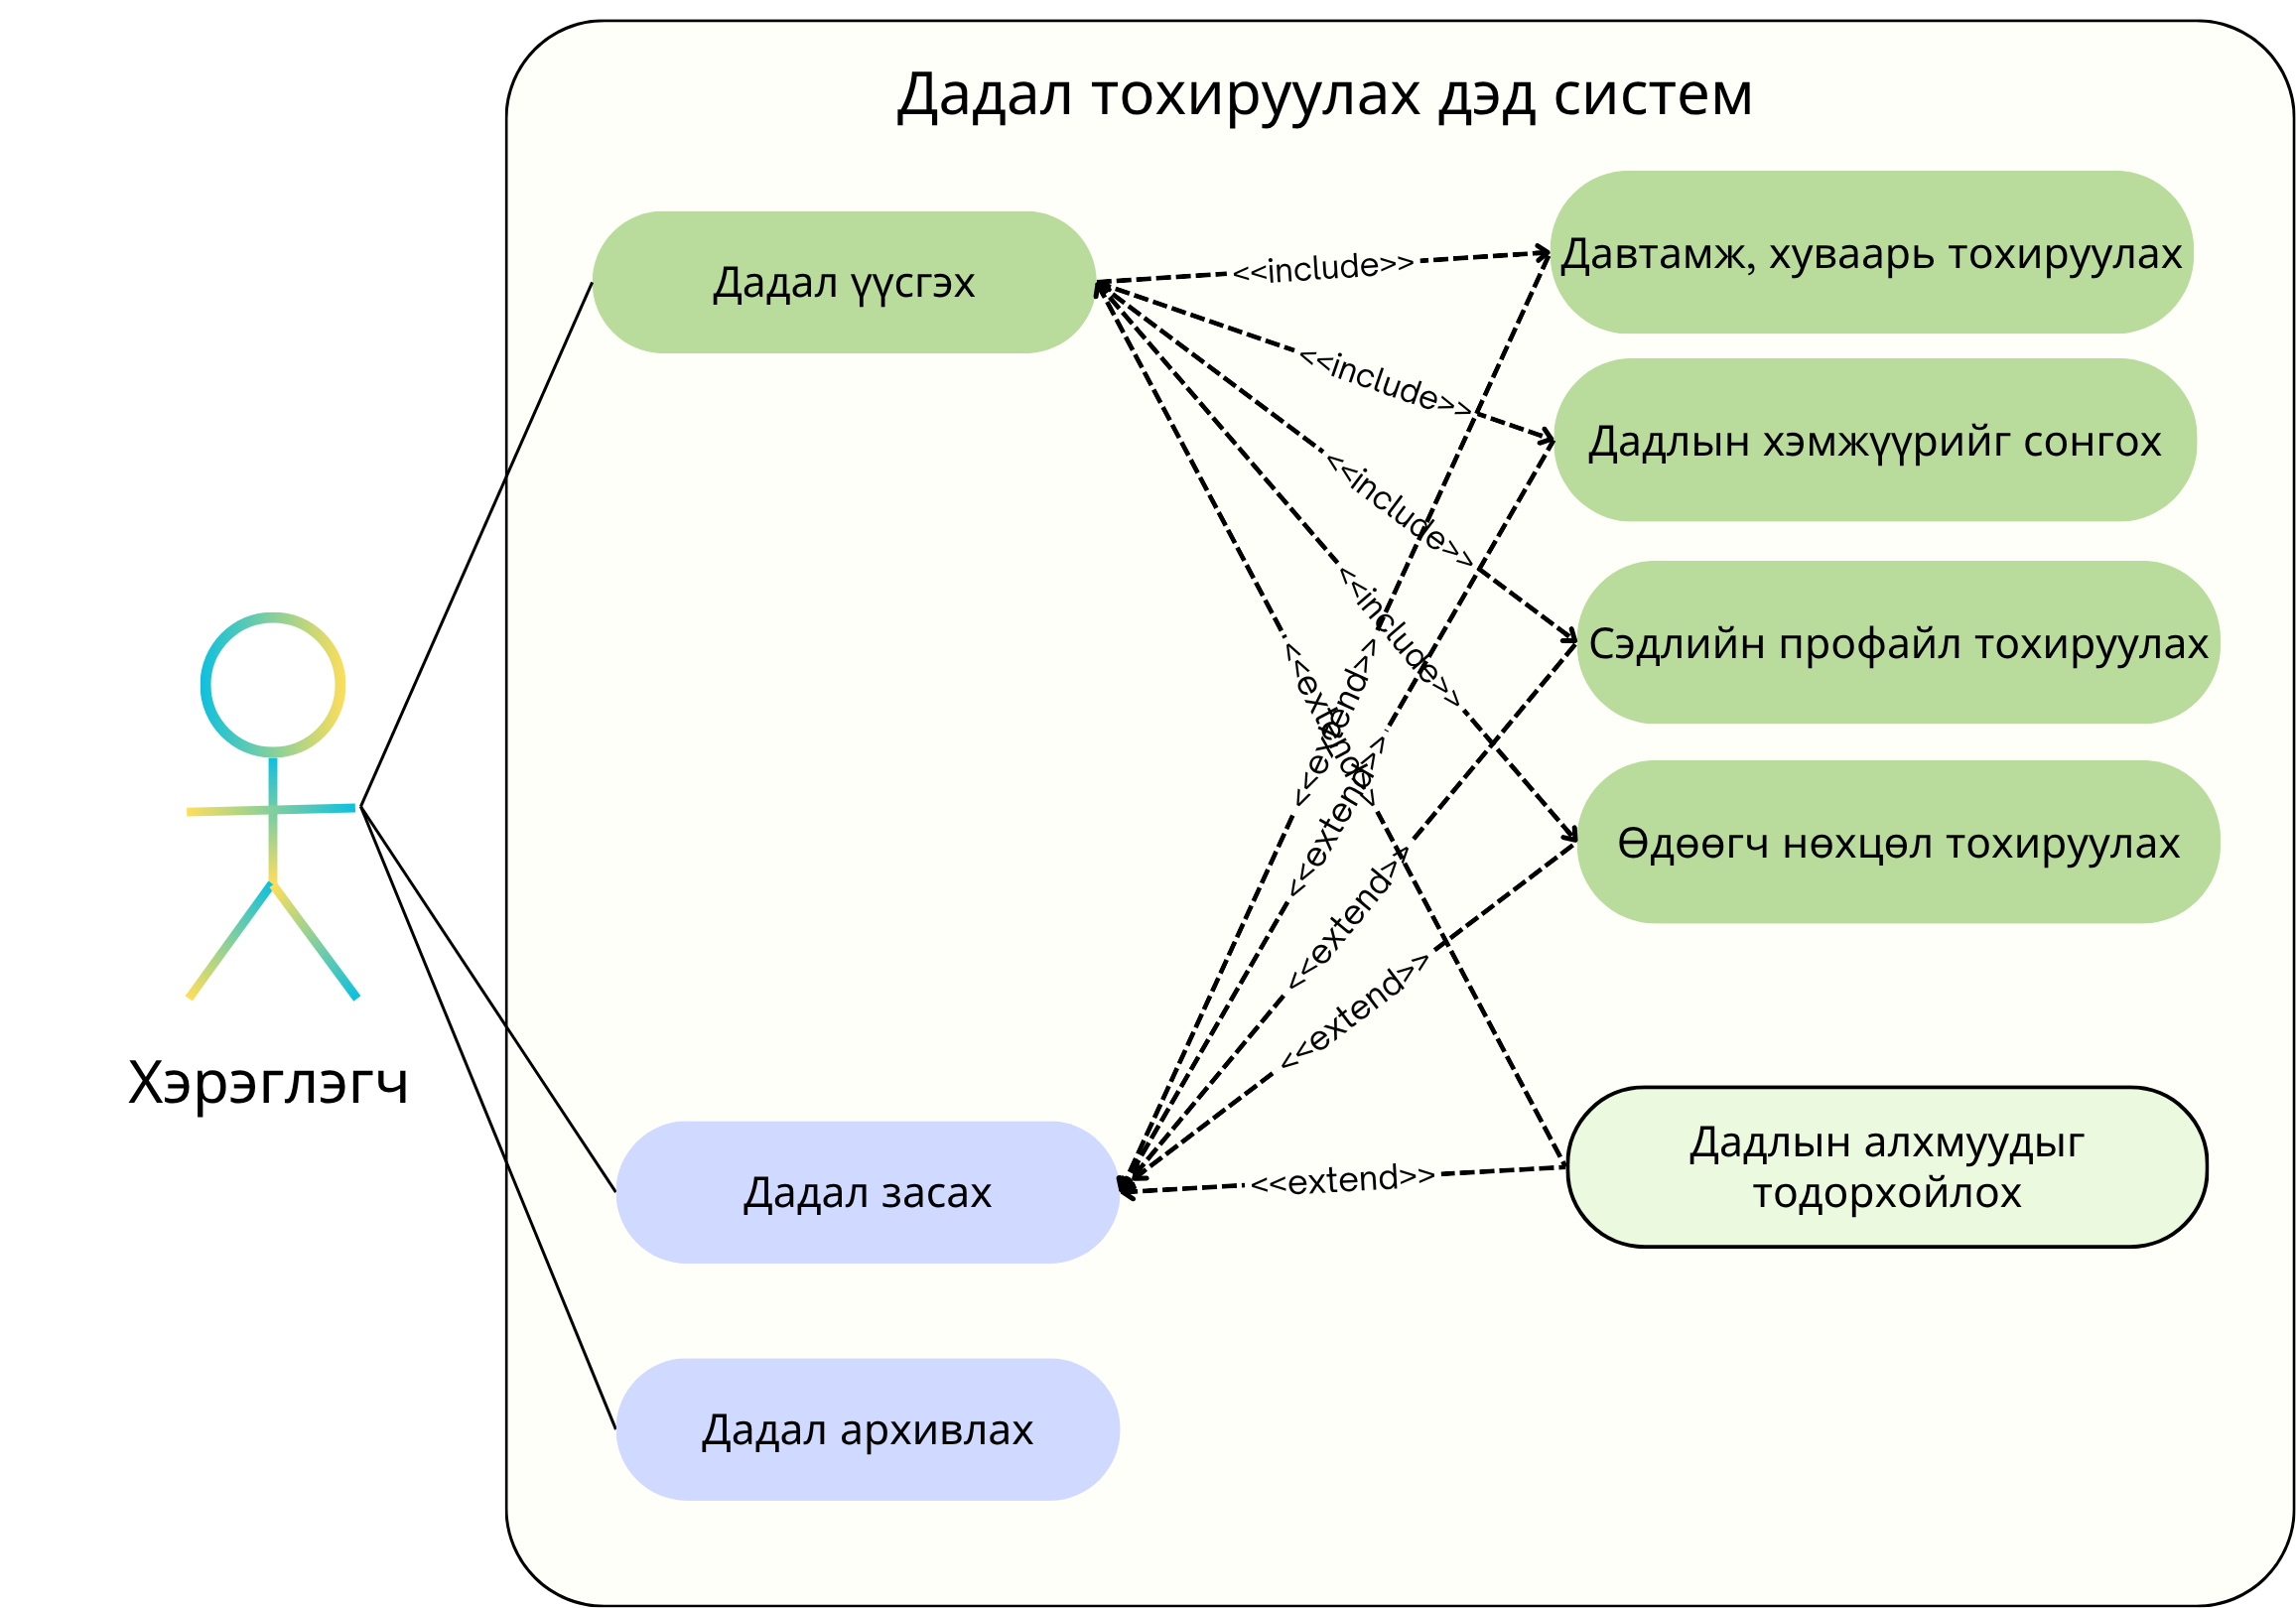
\includegraphics[width=0.84\textwidth]{images/HabitManagementUseCase.png}
    \caption{Дадал үүсгэх ба удирдах хэрэглээний тохиолдлын диаграмм}
\end{figure}

\begin{figure}[H]
    \centering
    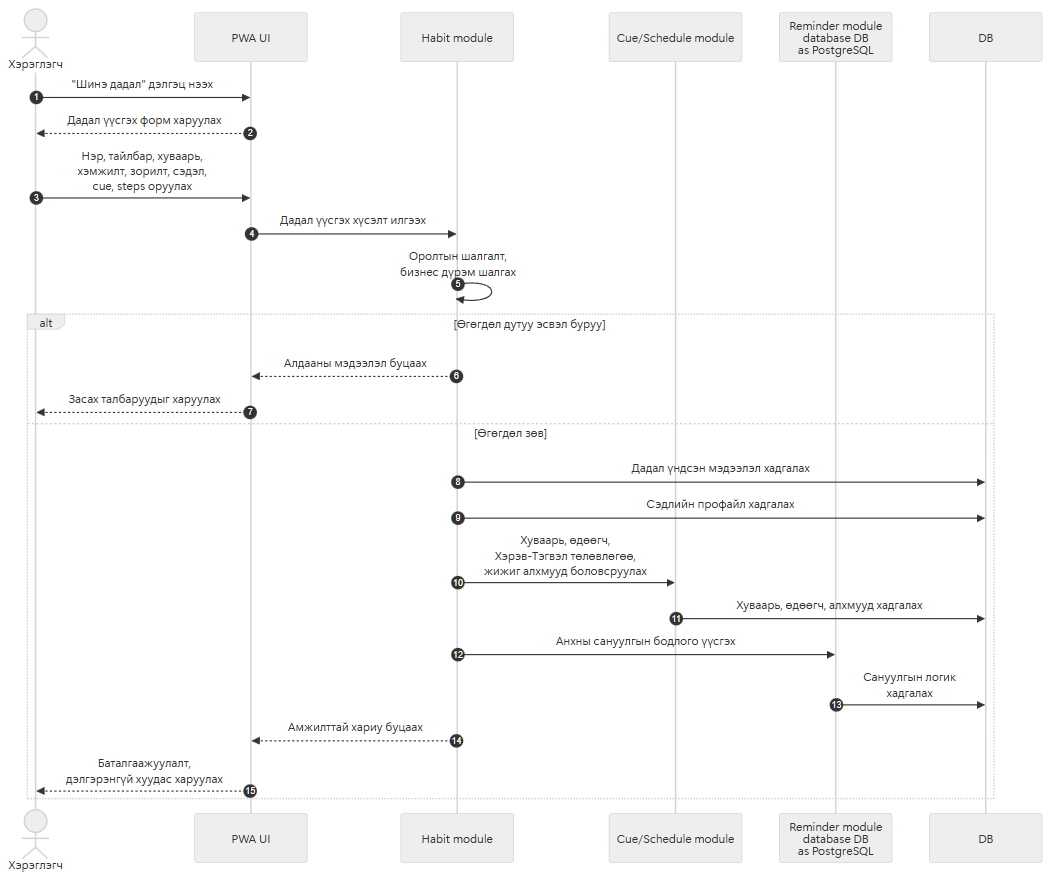
\includegraphics[width=\textwidth,height=0.82\textheight,keepaspectratio]{images/SequenceDiagram1.png}
    \caption{Дадал үүсгэх ба тохируулах дарааллын диаграмм}
\end{figure}

\begin{figure}[H]
    \centering
    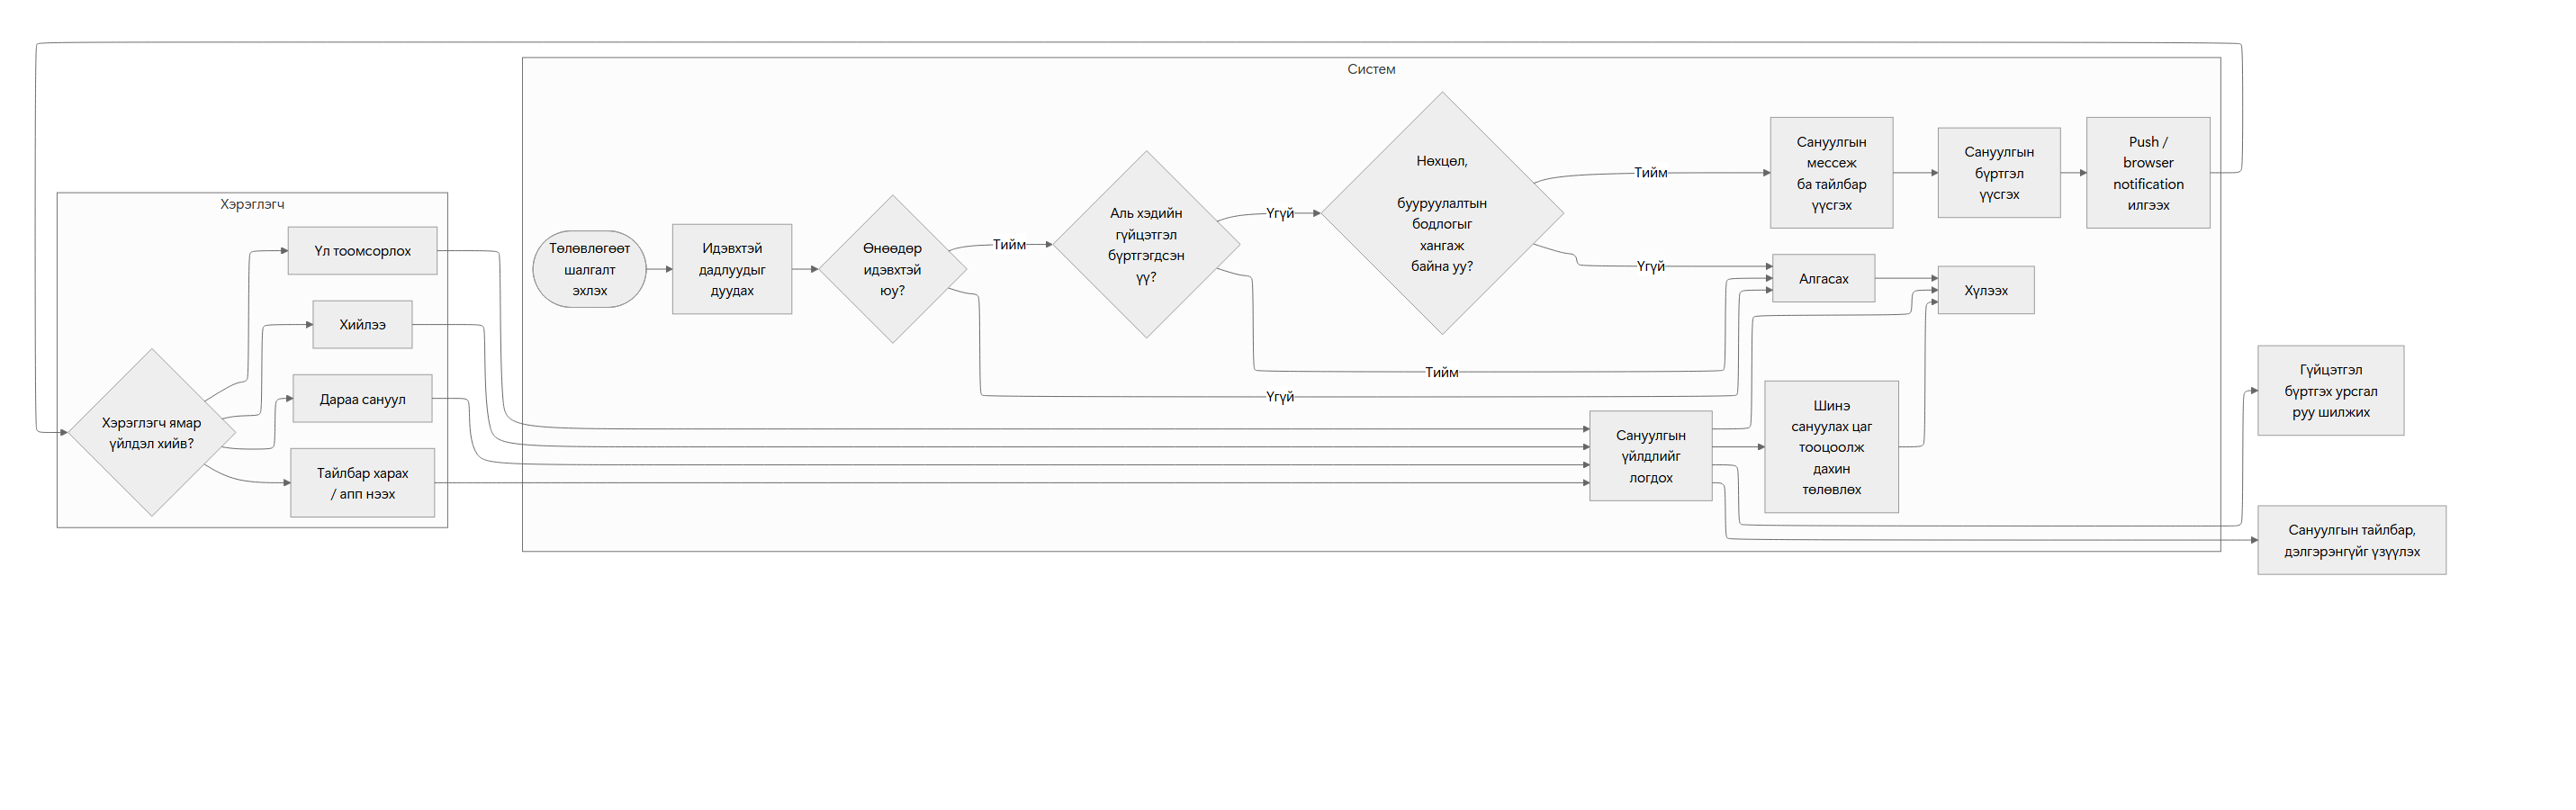
\includegraphics[width=\textwidth,height=0.82\textheight,keepaspectratio]{images/ActivityDiagram3.png}
    \caption{Нөхцөл байдалд суурилсан сануулга шийдвэрлэх ба хүргэх үйл ажиллагааны диаграмм}
\end{figure}

\begin{figure}[H]
    \centering
    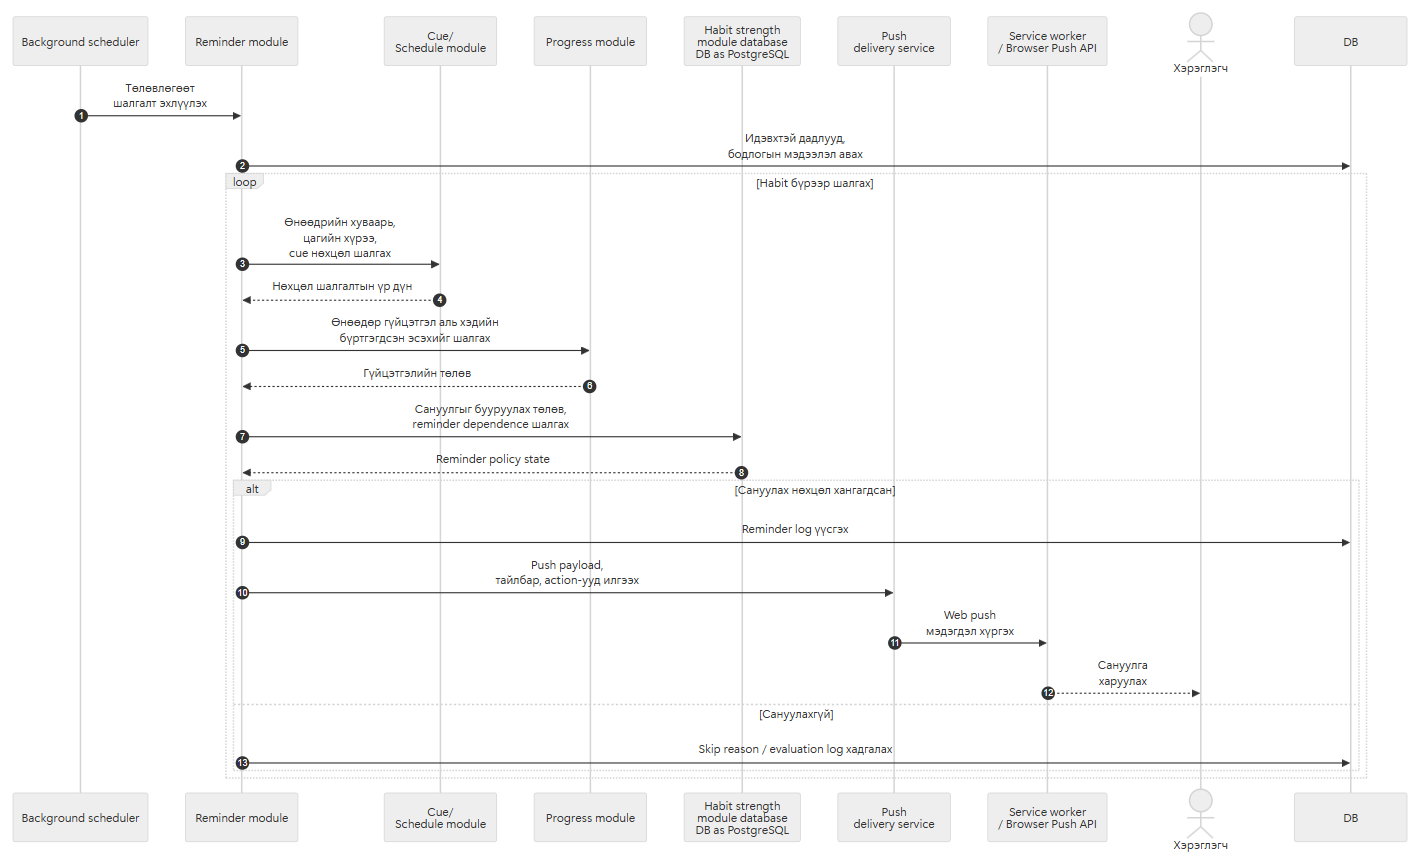
\includegraphics[width=\textwidth,height=0.82\textheight,keepaspectratio]{images/SequenceDiagram2.png}
    \caption{Нөхцөл байдалд суурилсан сануулга шийдвэрлэх ба хүргэх дарааллын диаграмм}
\end{figure}

\begin{figure}[H]
    \centering
    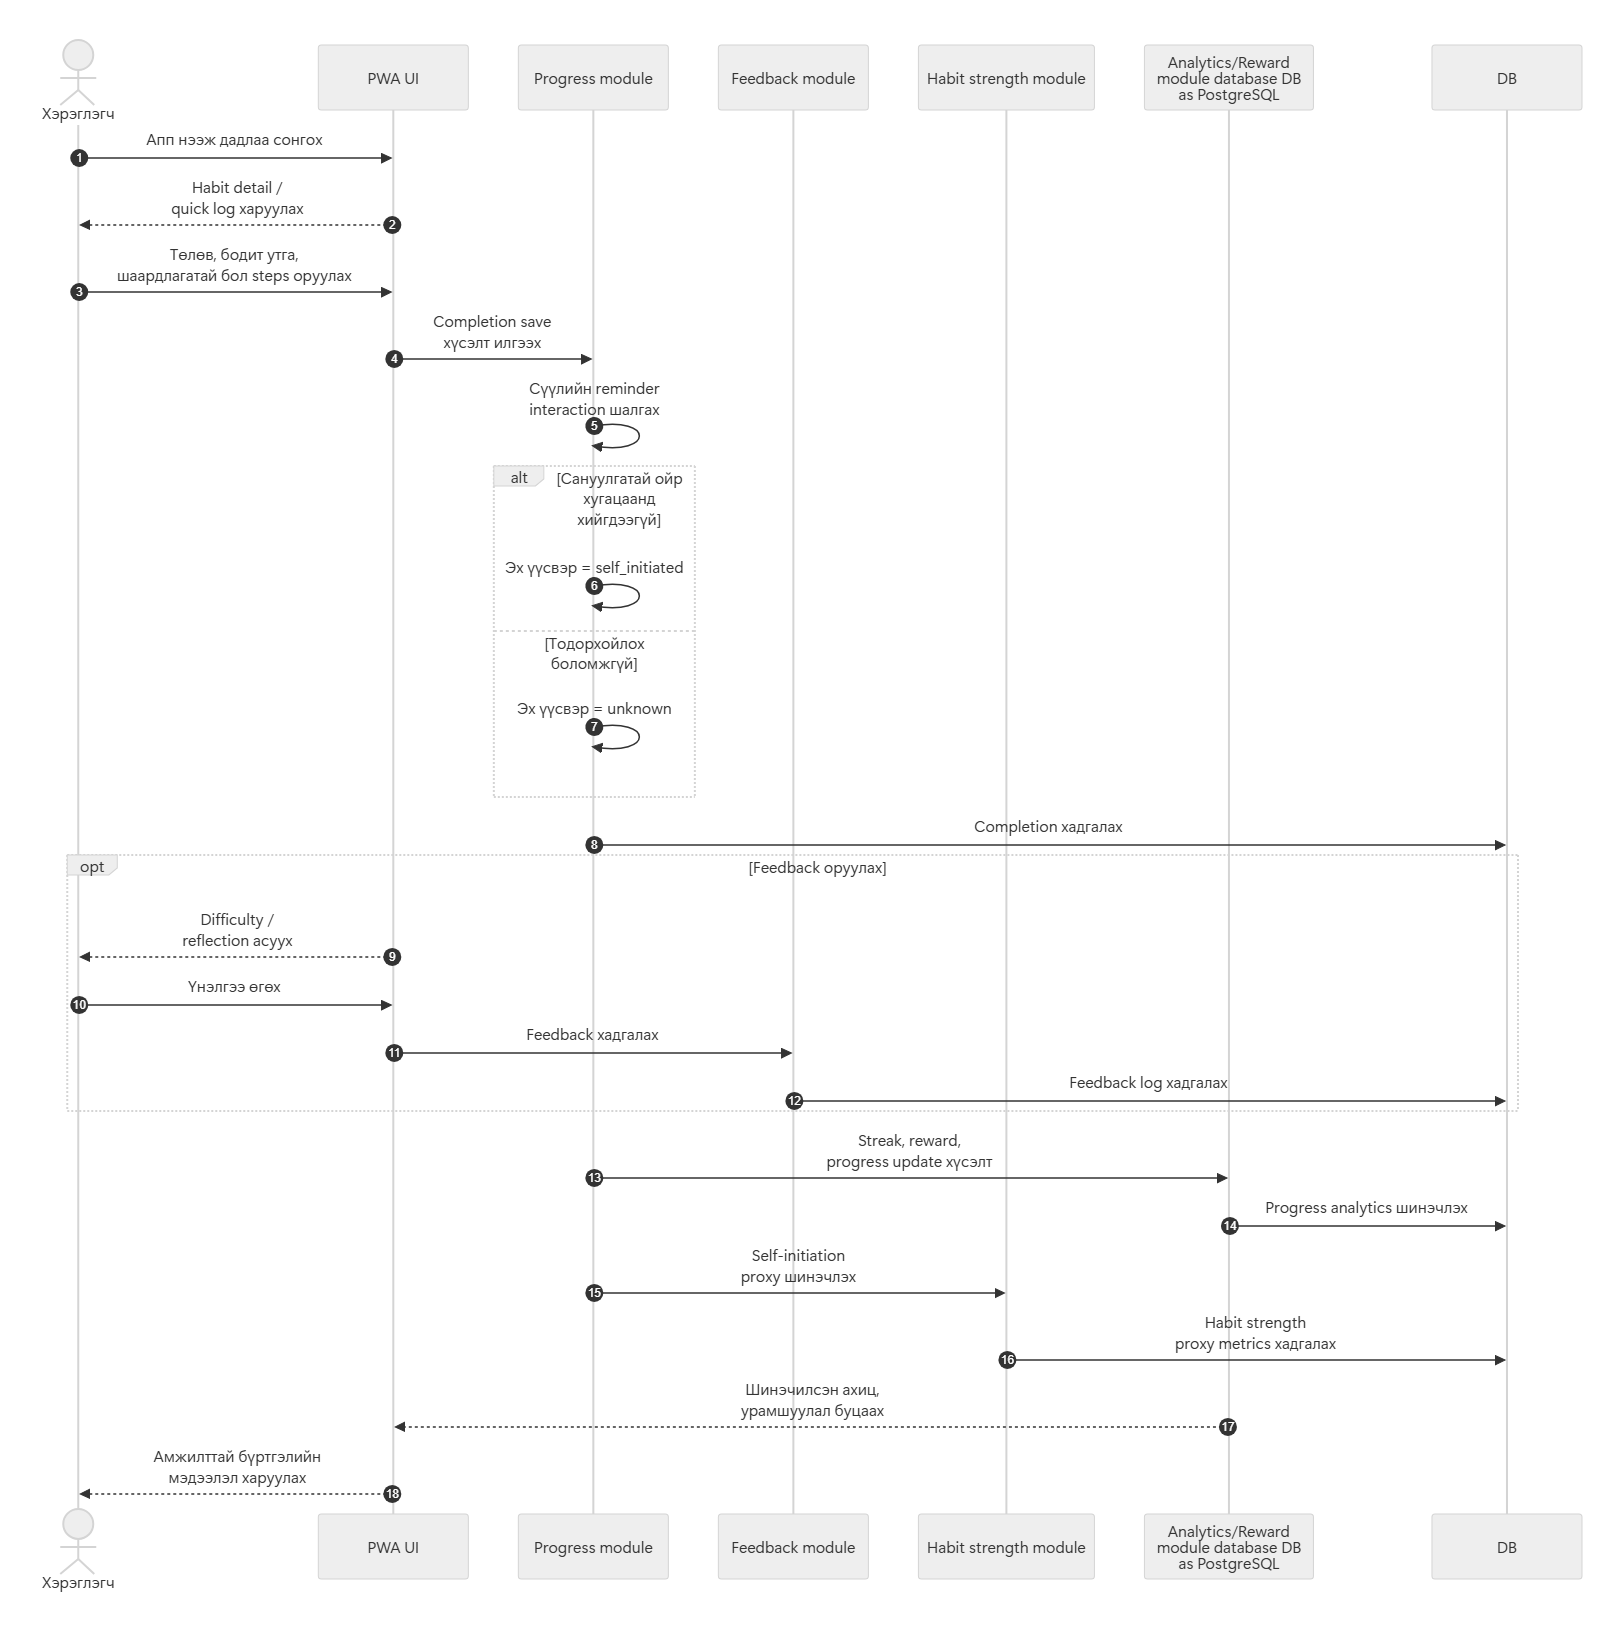
\includegraphics[width=\textwidth,height=0.82\textheight,keepaspectratio]{images/SequenceDiagram4.png}
    \caption{Сануулгагүйгээр өөрийн санаачилгатай гүйцэтгэл бүртгэх дарааллын диаграмм}
\end{figure}

\begin{figure}[H]
    \centering
    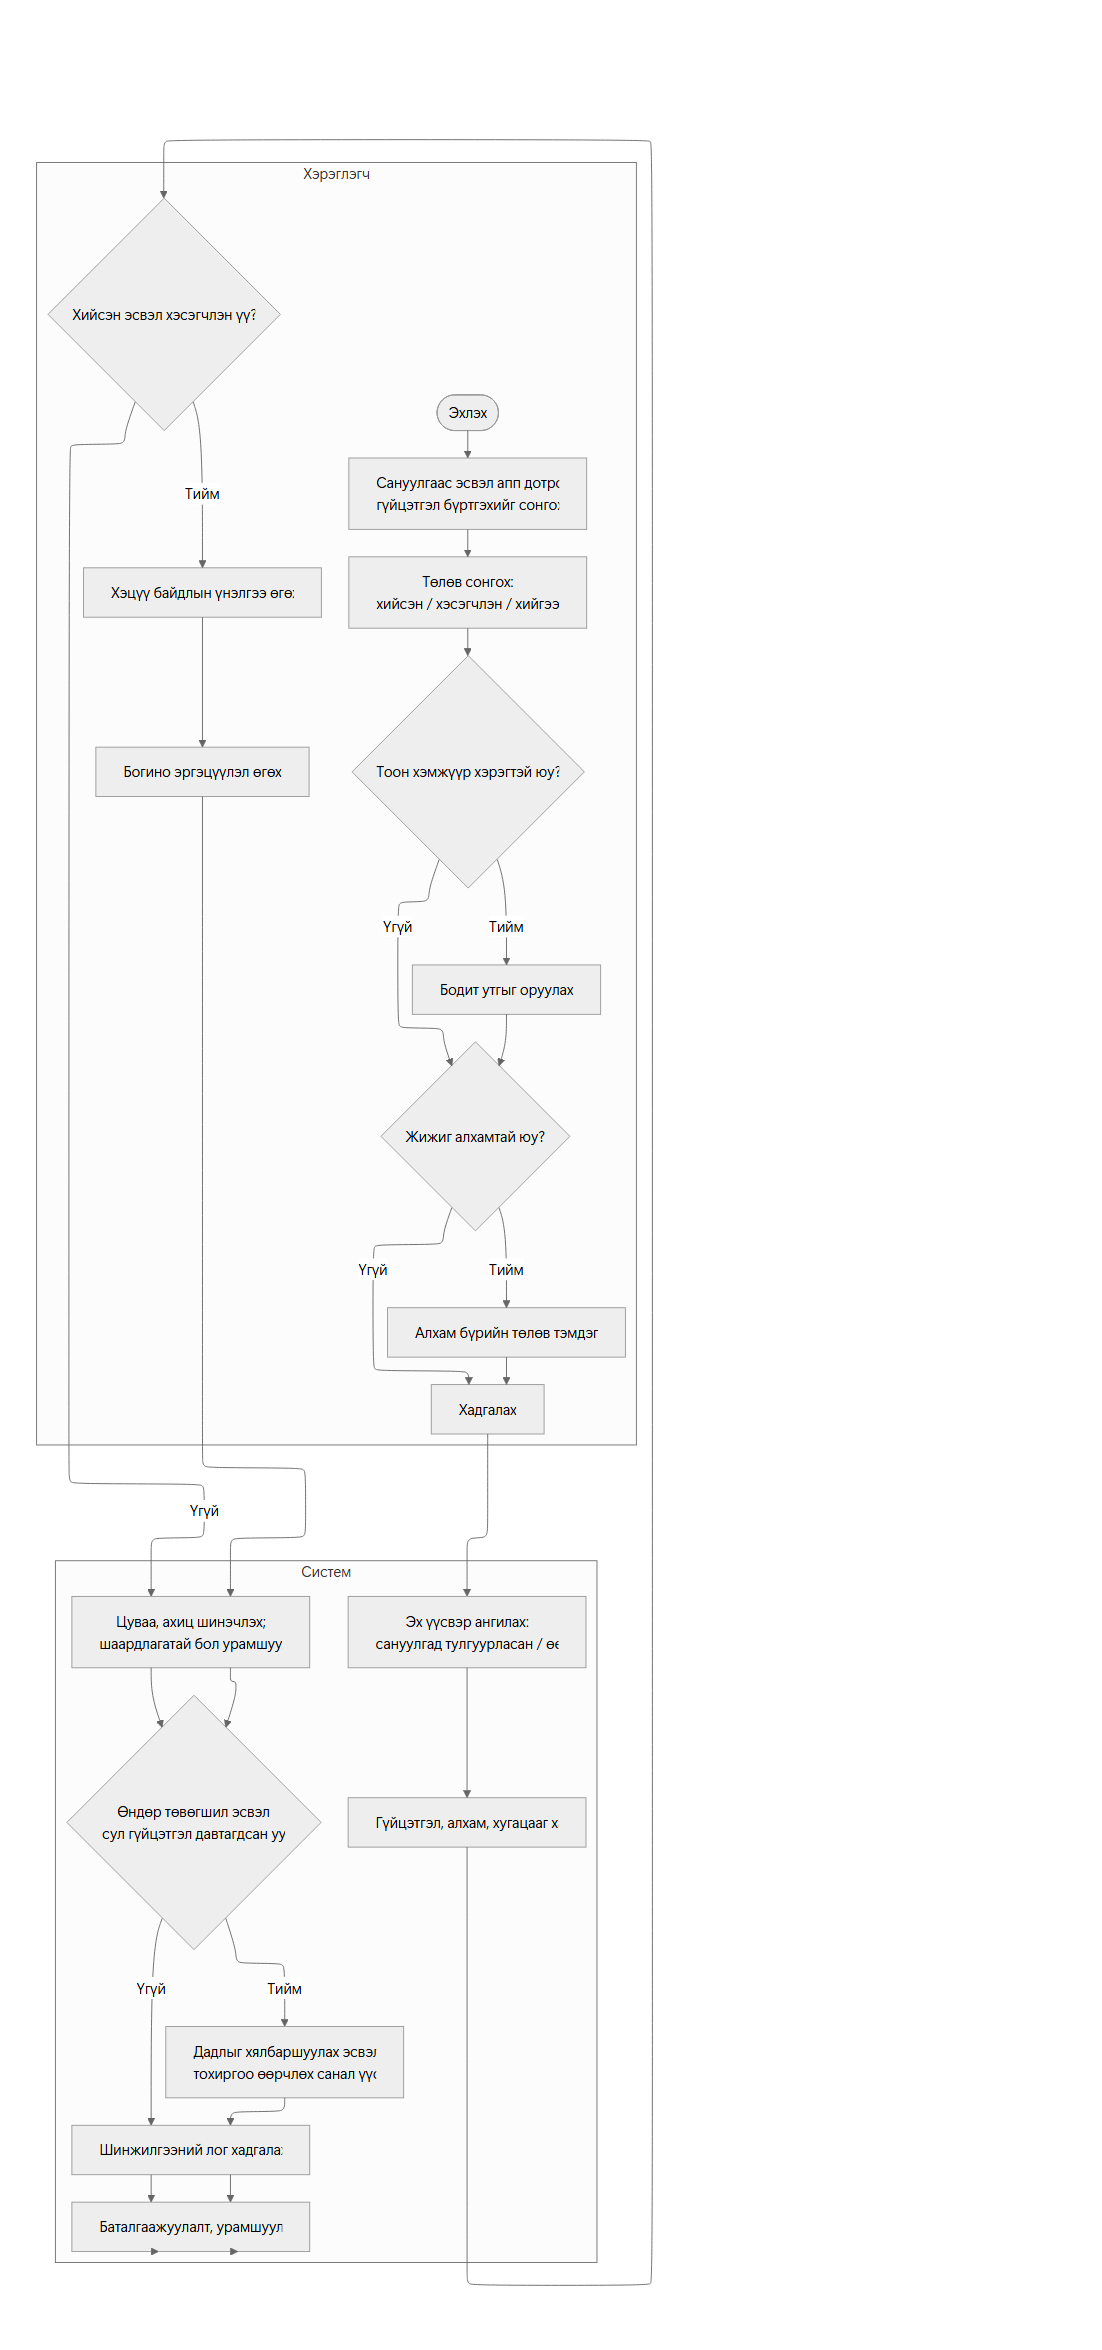
\includegraphics[width=\textwidth,height=0.82\textheight,keepaspectratio]{images/activityDiagram4.png}
    \caption{Гүйцэтгэл бүртгэх, санал сэтгэгдэл авах, урамшуулал идэвхжүүлэх үйл ажиллагааны диаграмм}
\end{figure}

\begin{figure}[H]
    \centering
    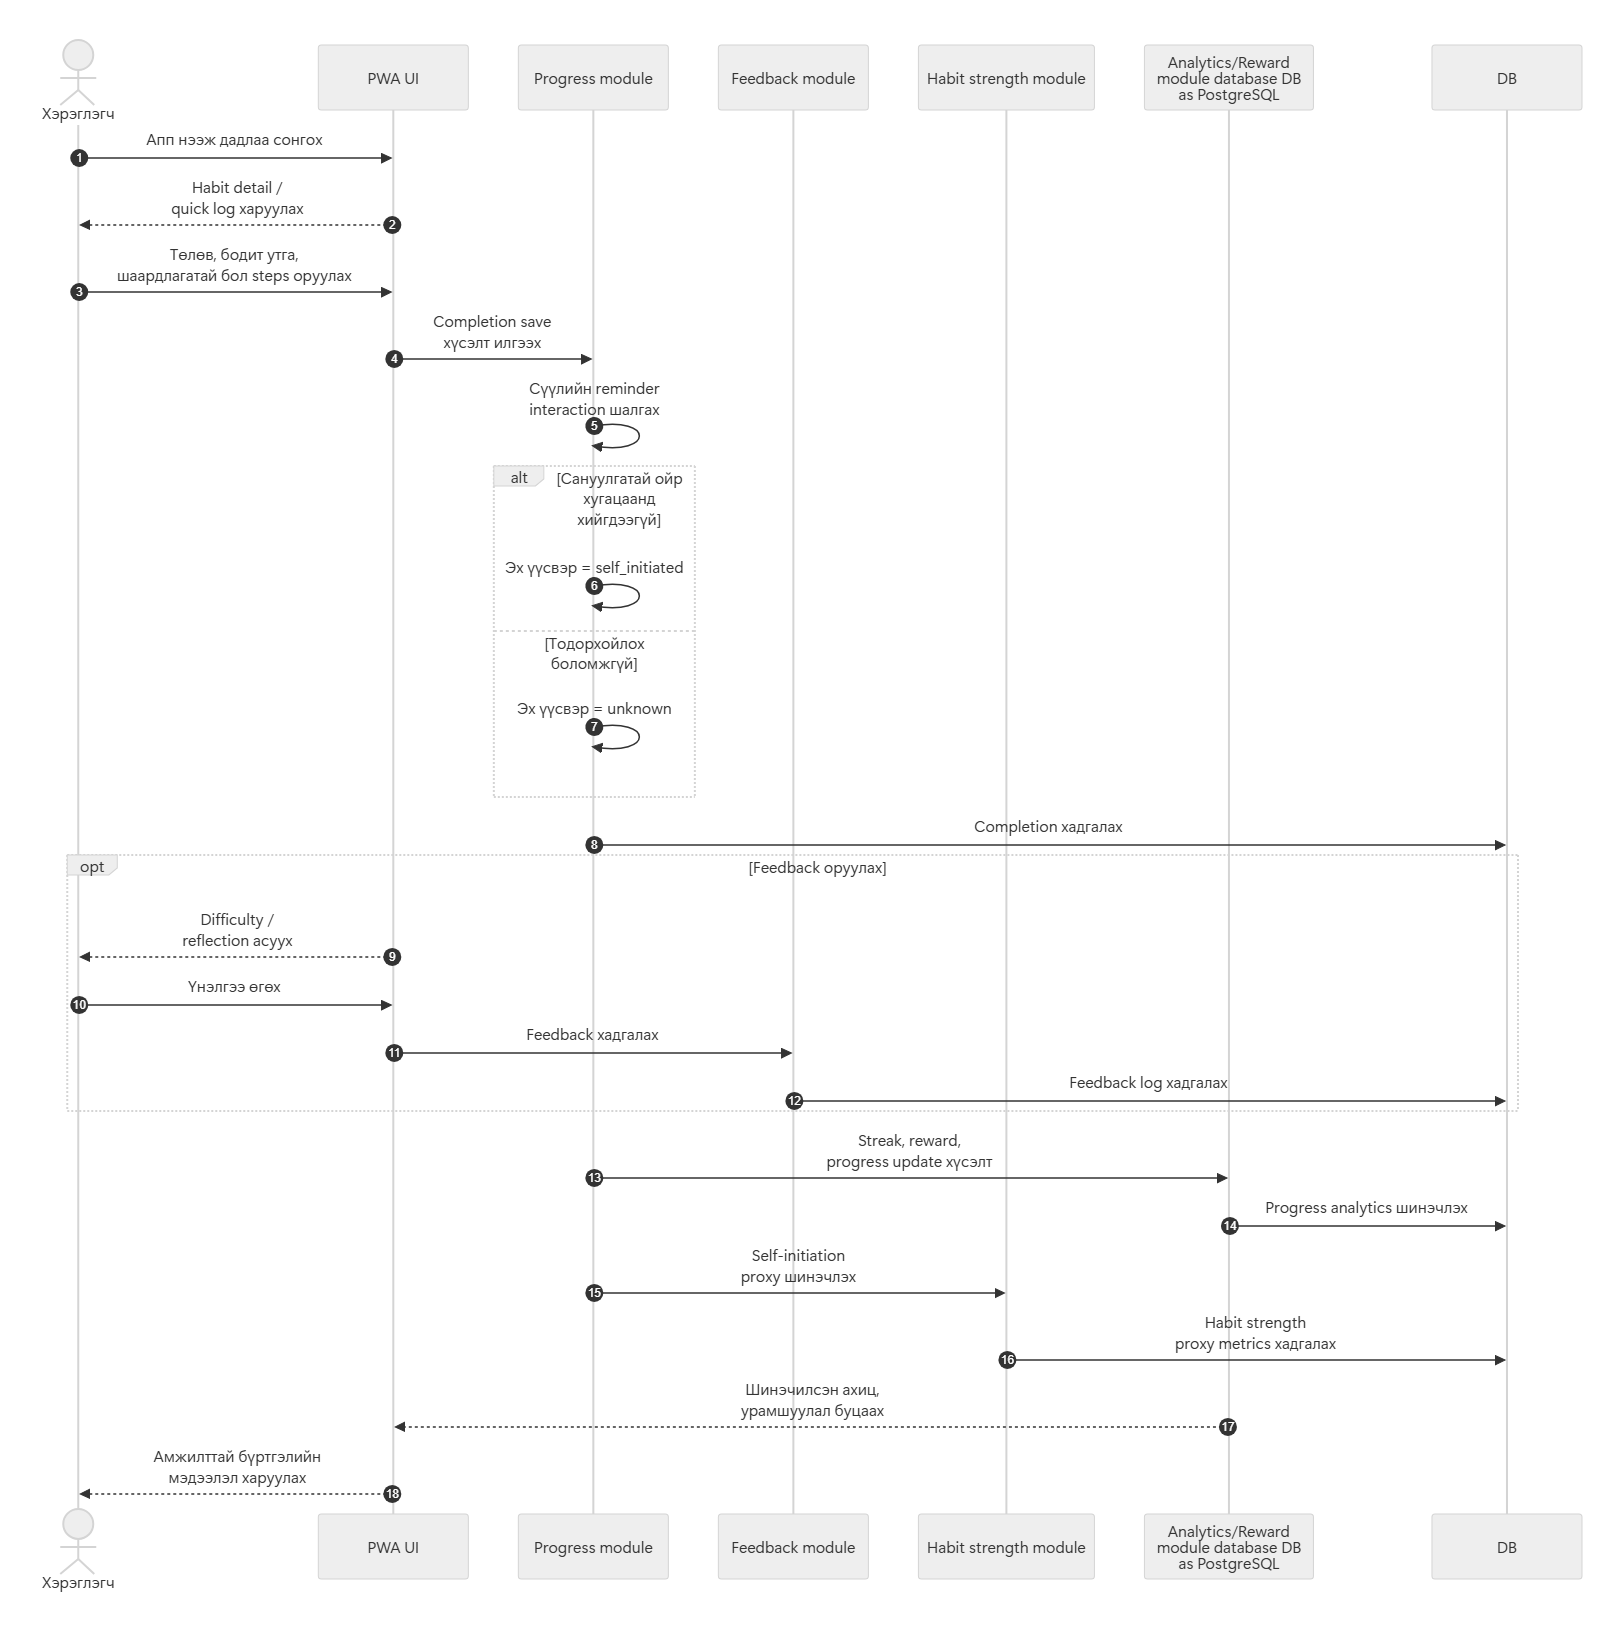
\includegraphics[width=\textwidth,height=0.82\textheight,keepaspectratio]{images/SequenceDiagram3.png}
    \caption{Сануулгад хариулах ба гүйцэтгэл бүртгэх дарааллын диаграмм}
\end{figure}

\begin{figure}[H]
    \centering
    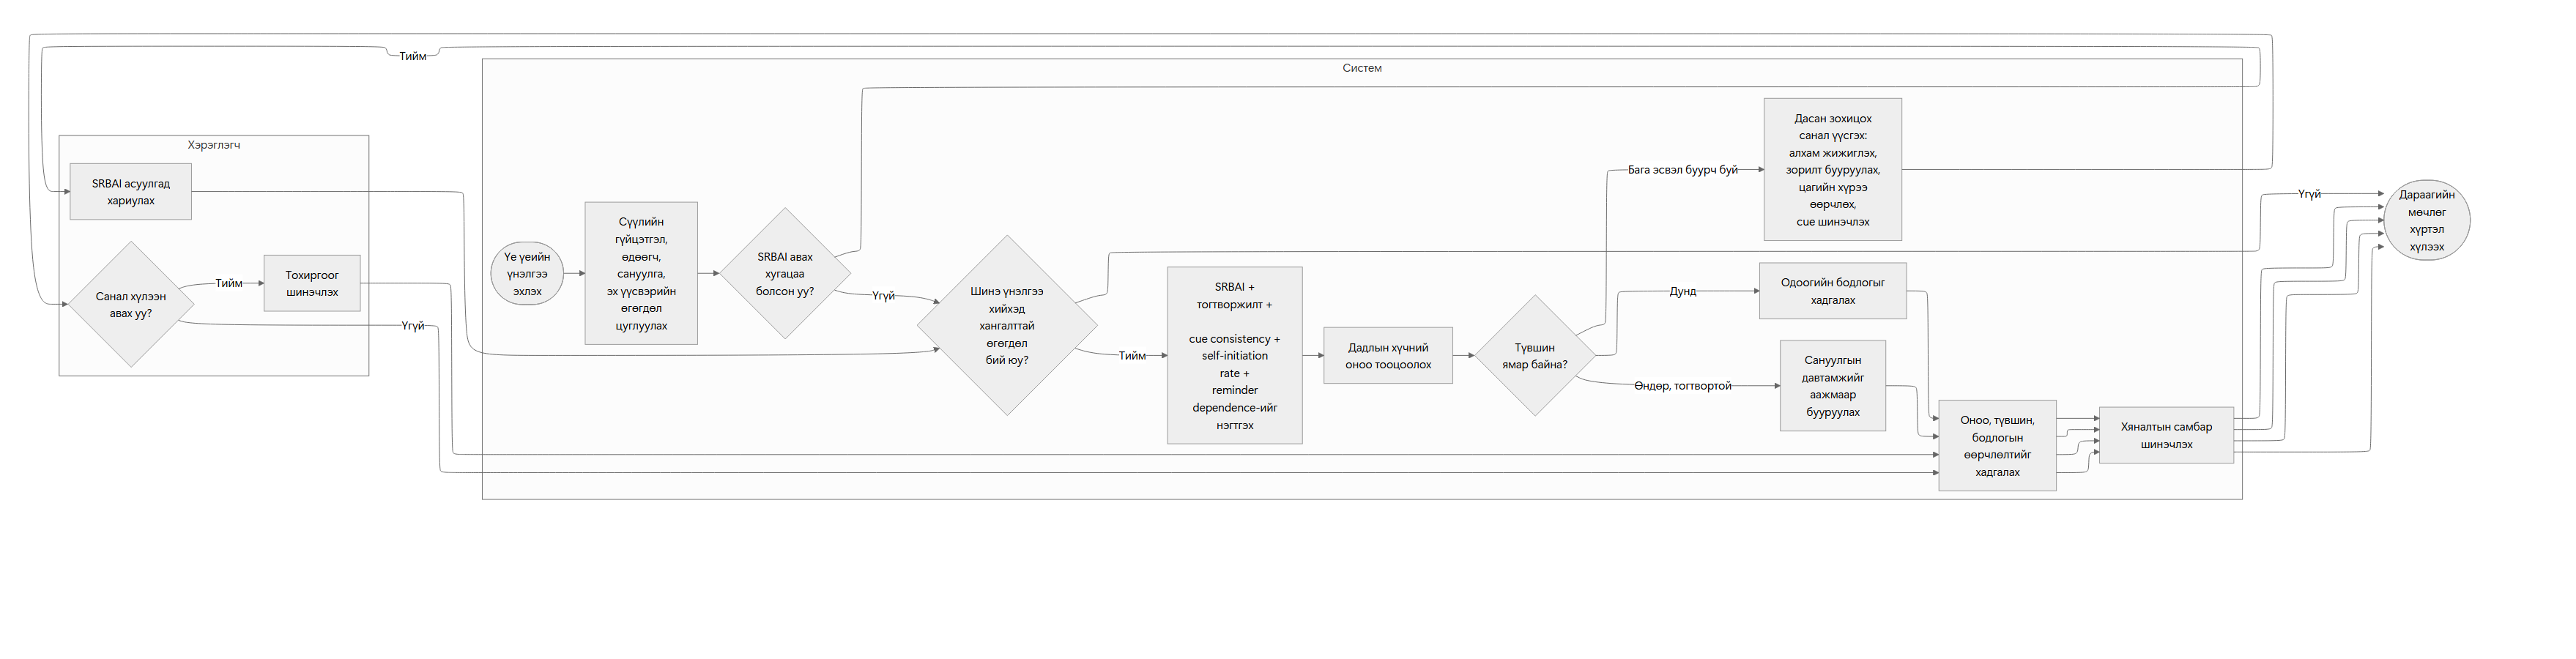
\includegraphics[width=\textwidth,height=0.82\textheight,keepaspectratio]{images/ActivityDiagram5.png}
    \caption{Дадлын хүчний үнэлгээ, сануулгын бодлого шинэчлэх ба дасан зохицох үйл ажиллагааны диаграмм}
\end{figure}

\begin{figure}[H]
    \centering
    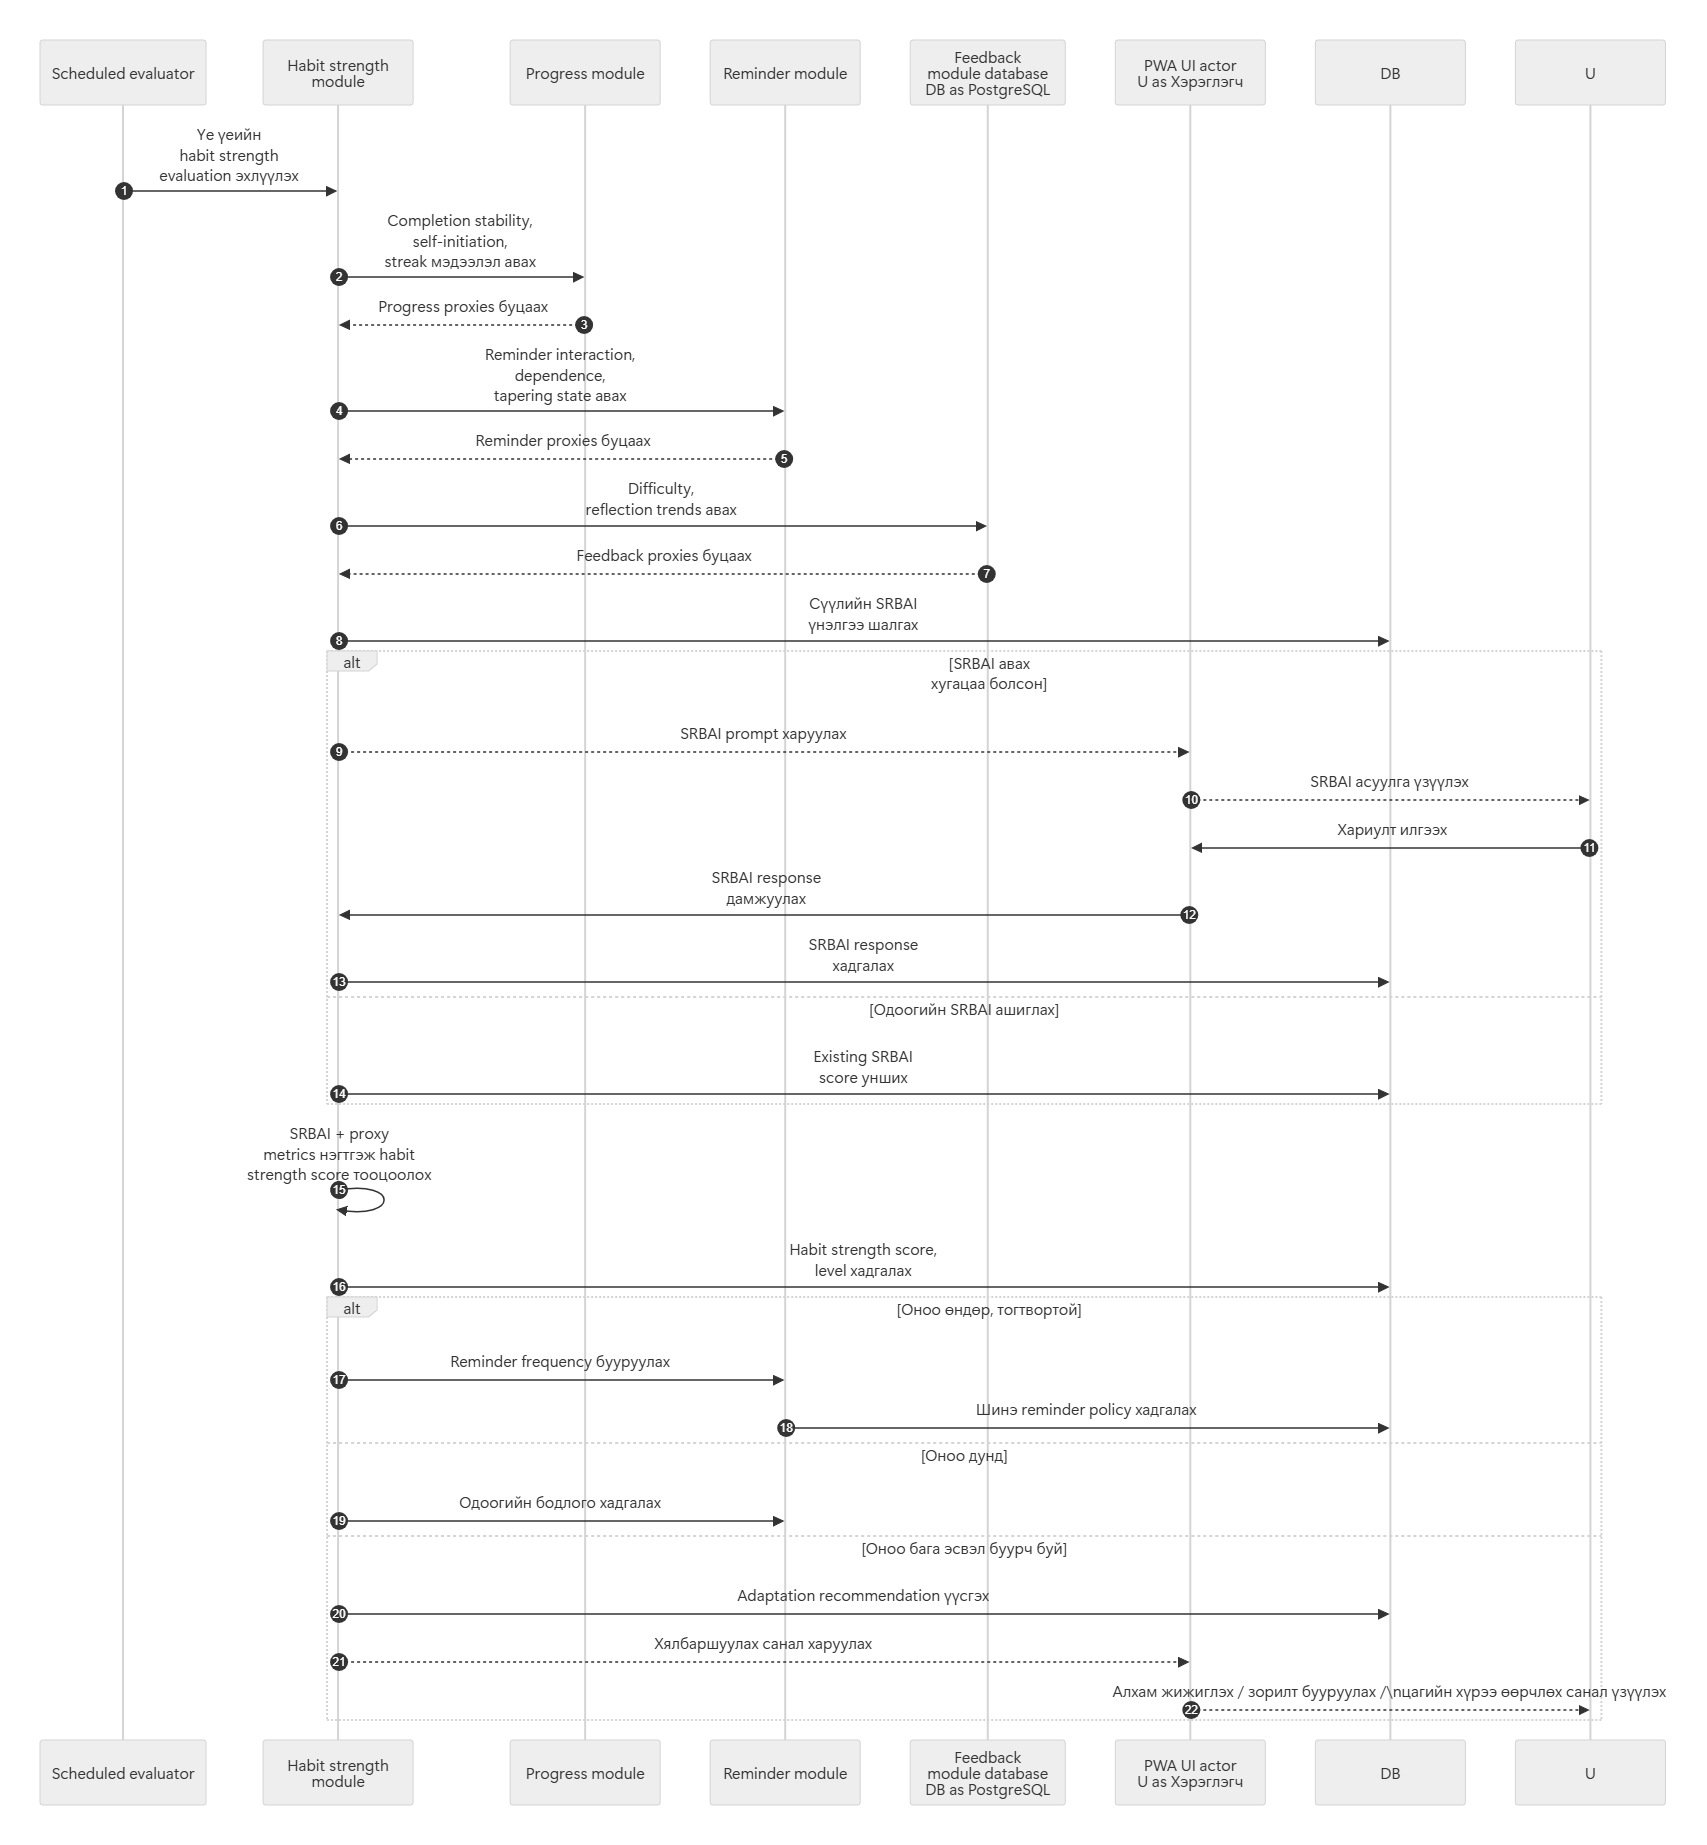
\includegraphics[width=\textwidth,height=0.82\textheight,keepaspectratio]{images/SequenceDiagram5.png}
    \caption{SRBAI үнэлгээ, дадлын хүч тооцоолох ба дасан зохицох дарааллын диаграмм}
\end{figure}

\section{Туршилтын дэлгэрэнгүй хэмжигдэх үзүүлэлтүүд}

\begin{table}[htbp]
\centering
\small
\setlength{\tabcolsep}{4pt}
\begin{tabular}{|L{4.0cm}|L{8.8cm}|}
\hline
\textbf{Үзүүлэлтийн бүлэг} & \textbf{Хэмжигдэх үндсэн үзүүлэлтүүд} \\
\hline
Өдөөгч дохио ба сануулга & Өдөөгч нөхцөл тохируулсан хувь, сануулга нээсэн хувь, сануулгад үйлдэл сонгосон хувь, сануулгын үйлдлийн тархалт, сануулгын цаг тохиромжтой байсан хувь, сануулгын давтамжийн өөрчлөлт \\
\hline
Сэдэл ба эргэцүүлэл & Сэдлийн профайл бүрдүүлсэн хувь, ашиг тусын мэдээлэл үзсэн хувь, эргэцүүлэл бөглөсөн хувь, зорилготой нийцэж буй субъектив үнэлгээ \\
\hline
Гүйцэтгэл ба төвөгшил & Нийт гүйцэтгэлийн хувь, хэсэгчлэн гүйцэтгэлийн хувь, гүйцэтгэл бүртгэхэд зарцуулсан хугацаа, жижиг алхмын гүйцэтгэлийн хувь, ``хэрэв--тэгвэл'' төлөвлөгөө үүсгэсэн хувь, хэцүү байдлын оноо, хялбаршуулах санал хүлээн авсан хувь \\
\hline
Тогтворжилт ба дотооджилт & Сануулгагүй нөхцөл дэх гүйцэтгэлийн хувь, тасралтгүй гүйцэтгэлийн цувааны урт, сэргээх боломж ашигласан хувь, автоматжилтын оноо, дадлын хүчний оноо, сануулгаас хэт хараат байдлын үзүүлэлт \\
\hline
Хэрэглээ ба оролцоо & 1, 7, 30 дахь өдрийн эргэн ирэлтийн үзүүлэлт, ахицын өөрчлөлтийн чиг хандлага, хуваалцах үйлдлийн хувь \\
\hline
\end{tabular}
\caption{Хэмжигдэх үндсэн үзүүлэлтүүдийн дэлгэрэнгүй хүснэгт}
\end{table}


\singlespace
\addcontentsline{toc}{part}{ЭХ СУРВАЛЖУУД}
\begin{thebibliography}{99}
    \bibitem{ref1}
    Wood, W., \& R\"unger, D. (2016). Psychology of habit. \textit{Annual Review of Psychology}, 67, 289--314.

    \bibitem{ref2}
    Duhigg, C. (2012). \textit{The Power of Habit: Why We Do What We Do in Life and Business}. Random House.

    \bibitem{ref3}
    Clear, J. (2018). \textit{Atomic Habits}. Avery.

    \bibitem{ref4}
    Fogg, B. J. (2009). A behavior model for persuasive design. In \textit{Proceedings of the 4th International Conference on Persuasive Technology}.

    \bibitem{ref5}
    Renfree, I., Harrison, D., Marshall, P., Stawarz, K., \& Cox, A. (2016). Don't kick the habit: The role of dependency in habit formation apps. In \textit{CHI EA '16 Proceedings of the 2016 CHI Conference Extended Abstracts on Human Factors in Computing Systems} (pp. 2932--2939). ACM. \url{https://doi.org/10.1145/2851581.2892495}

    \bibitem{ref6}
    Lally, P., van Jaarsveld, C. H. M., Potts, H. W. W., \& Wardle, J. (2010). How are habits formed: Modelling habit formation in the real world. \textit{European Journal of Social Psychology}, 40(6), 998--1009.

    \bibitem{ref8}
    Verplanken, B., \& Orbell, S. (2003). Reflections on past behavior: A self-report index of habit strength. \textit{Journal of Applied Social Psychology}, 33(6), 1313--1330.

    \bibitem{ref9}
    Gardner, B., Abraham, C., Lally, P., \& de Bruijn, G.-J. (2012). Towards parsimony in habit measurement: Testing the Self-Report Behavioral Automaticity Index. \textit{International Journal of Behavioral Nutrition and Physical Activity}, 9, 102.

    \bibitem{ref11}
    Stawarz, K., Cox, A. L., \& Blandford, A. (2015). Beyond self-tracking and reminders: Designing smartphone apps that support habit formation. In \textit{Proceedings of the 33rd Annual ACM Conference on Human Factors in Computing Systems}.

    \bibitem{ref13}
    Hamari, J., Koivisto, J., \& Sarsa, H. (2014). Does gamification work? A literature review of empirical studies on gamification. In \textit{Proceedings of the 47th Hawaii International Conference on System Sciences}.

    \bibitem{ref14}
    Mekler, E. D., Br\"uhlmann, F., Tuch, A. N., \& Opwis, K. (2017). Towards understanding the effects of individual gamification elements on intrinsic motivation and performance. \textit{Computers in Human Behavior}, 71, 525--534.

    \bibitem{ref15}
    Oinas-Kukkonen, H., \& Harjumaa, M. (2009). Persuasive systems design: Key issues, process model, and system features. \textit{Communications of the Association for Information Systems}, 24(1), 28.

    \bibitem{ref16}
    Nahum-Shani, I., Smith, S. N., Spring, B. J., Collins, L. M., Witkiewitz, K., Tewari, A., \& Murphy, S. A. (2018). Just-in-time adaptive interventions (JITAIs) in mobile health: Key components and design principles for ongoing health behavior support. \textit{Annals of Behavioral Medicine}, 52(6), 446--462.

    \bibitem{pavlov1927}
    Pavlov, I. P. (1927). \textit{Conditioned Reflexes: An Investigation of the Physiological Activity of the Cerebral Cortex}. London: Oxford University Press.

    \bibitem{skinner1938}
    Skinner, B. F. (1938). \textit{The Behavior of Organisms: An Experimental Analysis}. New York: Appleton-Century.

    \bibitem{ref17}
    Loop Habit Tracker. (2026). \textit{Loop Habit Tracker}. Retrieved March 19, 2026, from \url{https://loophabits.org/}

    \bibitem{ref18}
    Crunchy Bagel. (2026). \textit{STREAKS}. Retrieved March 19, 2026, from \url{https://streaksapp.com/}

    \bibitem{ref19}
    Habitica. (2026). \textit{Habitica: Gamify your life}. Retrieved March 19, 2026, from \url{https://habitica.com/static/home}
\end{thebibliography}

\end{document}
